\documentclass[11pt]{article}
\usepackage[margin=2cm]{geometry}
\usepackage{amsmath,amssymb}
\usepackage{graphicx}
\usepackage{booktabs}
\usepackage{array}
\usepackage{xcolor}
\usepackage[breakable]{tcolorbox}
\usepackage{enumitem}
\usepackage[hidelinks]{hyperref}
\allowdisplaybreaks
\setlength{\parindent}{0pt}
\setlength{\parskip}{4pt}
\definecolor{stepc}{HTML}{1F4E9E}
\definecolor{ansc}{HTML}{0B6E4F}
\newcommand{\solstep}[2]{\par\medskip{\color{stepc}\textbf{Step #1 --- #2}}\par\nopagebreak}
\newtcolorbox{probbox}[1]{colback=white,colframe=black!55,fonttitle=\bfseries,title={#1}}
\newtcolorbox{ansbox}{breakable,colback=ansc!6,colframe=ansc,fonttitle=\bfseries,title={Answer}}
\newtcolorbox{cardbox}[1]{breakable,colback=stepc!4,colframe=stepc,fonttitle=\bfseries,title={#1}}
\graphicspath{{../../../output/lecture3/3B_diode_opamp/}}
\title{Set 3B: Op-Amp Circuits with Diodes}
\author{ECEN 325 --- Lecture 3 (Diodes) practice set}
\date{}
\begin{document}
\maketitle

\textbf{What this set trains.} The same state method as set 3A, now with ideal op-amps. In each assumed state an
op-amp either has negative feedback (virtual short) or has lost it because a diode in its feedback path is OFF; then
it runs open-loop and its output swings until a diode turns on (Sample Problem 5). Problems 1--6 are easy, 7--12
medium, 13--18 hard. Try each problem before looking at its solution.


\begin{cardbox}{The Lecture-3 pipeline (use it for every problem in this lecture)}
\textbf{Tools --- this is all the theory you need (plus the Lecture-1/2 tools):}
\begin{enumerate}[label=\textbf{T\arabic*},leftmargin=2.2em,itemsep=1pt]
\item \emph{Diode models.} Ideal: OFF $\Leftrightarrow V_D<0$ (open), ON $\Leftrightarrow I_D>0$ ($V_D=0$).
      Constant-voltage-drop (CVD): OFF $\Leftrightarrow V_D<0.7$\,V (open), ON $\Leftrightarrow I_D>0$ ($V_D=0.7$\,V source).
      Exponential: $I_D = I_S e^{V_D/nV_T}$, i.e. $V_D = nV_T\ln(I_D/I_S)$, $V_T\approx 25$\,mV.
\item \emph{State method.} Assume ON/OFF for every diode, solve the now-linear circuit (KCL, Lecture 2), then check
      the assumptions; each check is a condition on $V_i$. The valid states tile the $V_i$ axis.
\item \emph{Small signal.} Around a DC point $I_D$ the diode is a resistor $r_d = \frac{nV_T}{I_D}$
      (valid while $|v_d|\ll nV_T$). Capacitors: open at DC; $\frac{1}{sC}$ in AC; DC supplies are AC ground.
\item \emph{Rectifier with a filter capacitor} ($f=60$\,Hz, $T = \frac{1}{f}$ half-wave, $\frac{1}{2f}$ full-wave):
      peak $V_p=\hat V_S - (\text{diode drops in the path})$; ripple $V_r \approx V_p\frac{T}{RC}$;
      $I_{D,av} \approx I_L\left(1+\pi\sqrt{2V_p/V_r}\right)$, $I_{D,max}\approx I_L\left(1+2\pi\sqrt{2V_p/V_r}\right)$;
      PIV $=$ the largest reverse voltage a diode sees.
\end{enumerate}
\textbf{Steps:}
\begin{enumerate}[leftmargin=2.2em,itemsep=1pt]
\item \emph{Pick the model} stated in the problem.
\item \emph{Transfer characteristic:} for each ON/OFF state: replace the diodes, solve, check $\Rightarrow$ range of $V_i$;
      then join the pieces (they must meet at the breakpoints) and sketch.
\item \emph{Small signal:} DC operating point first, then $r_d$, then the AC circuit exactly as in Lectures 1--2,
      then add DC and AC.
\item \emph{Rectifiers:} peak $\to$ ripple (or $C$ for a given ripple) $\to$ diode currents $\to$ PIV $\to$ transformer ratio.
\end{enumerate}
\end{cardbox}

\section*{Problems}
\subsection*{Easy problems}
\begin{probbox}{Problem 3B.1 \hfill Easy}
For the circuit below (ideal op-amps), use the constant-voltage-drop model ($V_{D,on}=0.7$\,V). Find $V_o$ as a function of $V_i$ and sketch $V_o$ versus $V_i$.
\begin{center}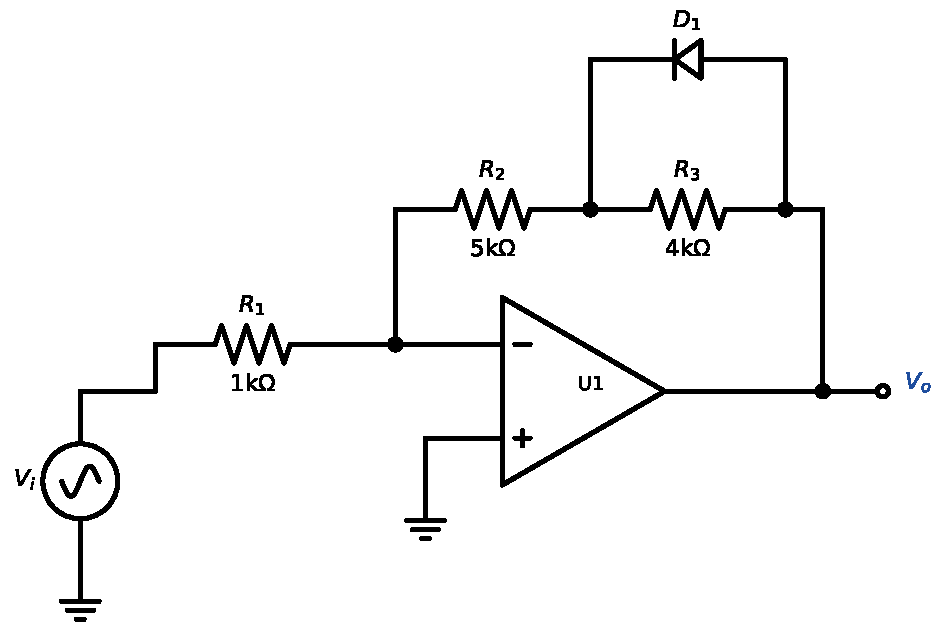
\includegraphics[width=\linewidth,height=5.6cm,keepaspectratio]{p01_circuit}\end{center}
\end{probbox}

\begin{probbox}{Problem 3B.2 \hfill Easy}
For the circuit below (ideal op-amps), use the constant-voltage-drop model ($V_{D,on}=0.7$\,V). Find $V_o$ as a function of $V_i$ and sketch $V_o$ versus $V_i$. Also sketch $V_o(t)$ for $V_i(t) = 1\sin(2\pi\cdot 1000\,t)$.
\begin{center}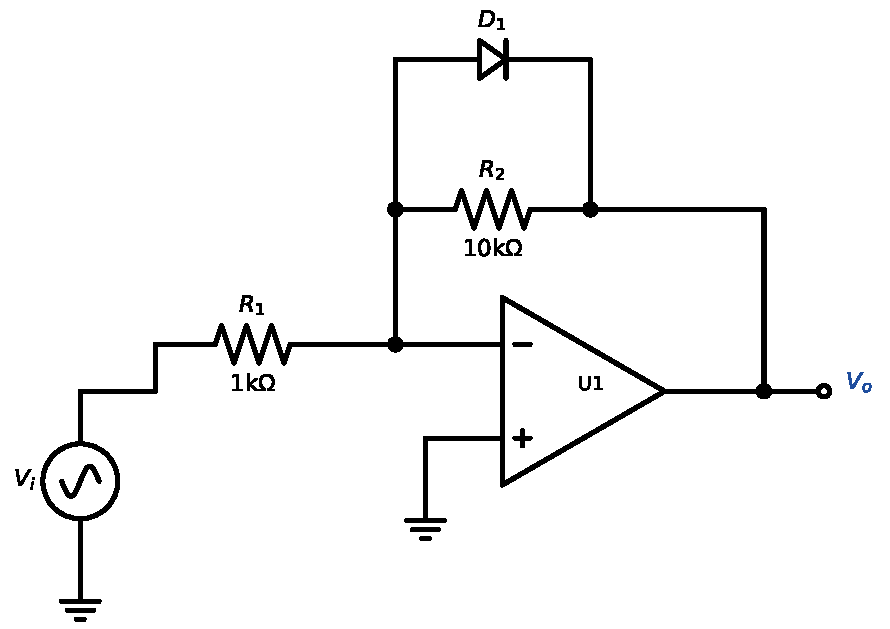
\includegraphics[width=\linewidth,height=5.6cm,keepaspectratio]{p02_circuit}\end{center}
\end{probbox}

\begin{probbox}{Problem 3B.3 \hfill Easy}
For the circuit below (ideal op-amps), use the constant-voltage-drop model ($V_{D,on}=0.7$\,V). Find $V_o$ as a function of $V_i$ and sketch $V_o$ versus $V_i$. Also sketch $V_o(t)$ for $V_i(t) = 2\sin(2\pi\cdot 500\,t)$.
\begin{center}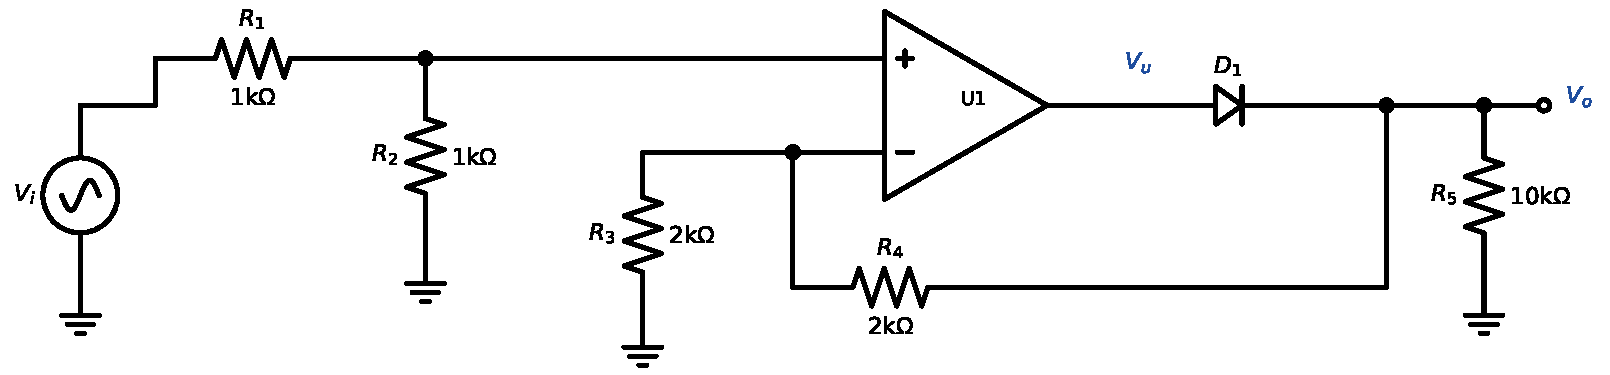
\includegraphics[width=\linewidth,height=5.6cm,keepaspectratio]{p03_circuit}\end{center}
\end{probbox}

\begin{probbox}{Problem 3B.4 \hfill Easy}
For the circuit below (ideal op-amps), use the constant-voltage-drop model ($V_{D,on}=0.7$\,V). Find $V_o$ as a function of $V_i$ and sketch $V_o$ versus $V_i$. Also sketch $V_o(t)$ for $V_i(t) = 1\sin(2\pi\cdot 1000\,t)$.
\begin{center}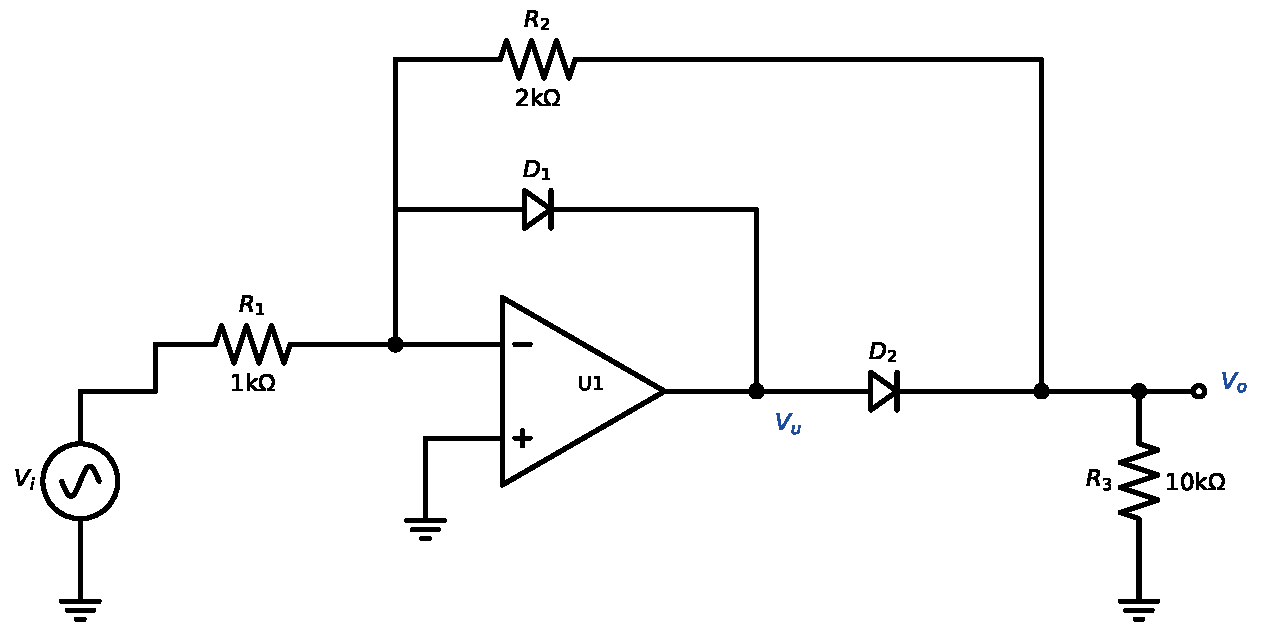
\includegraphics[width=\linewidth,height=5.6cm,keepaspectratio]{p04_circuit}\end{center}
\end{probbox}

\begin{probbox}{Problem 3B.5 \hfill Easy}
For the circuit below (ideal op-amps), use the constant-voltage-drop model ($V_{D,on}=0.7$\,V). Find $V_o$ as a function of $V_i$ and sketch $V_o$ versus $V_i$. Also sketch $V_o(t)$ for $V_i(t) = 3\sin(2\pi\cdot 1000\,t)$.
\begin{center}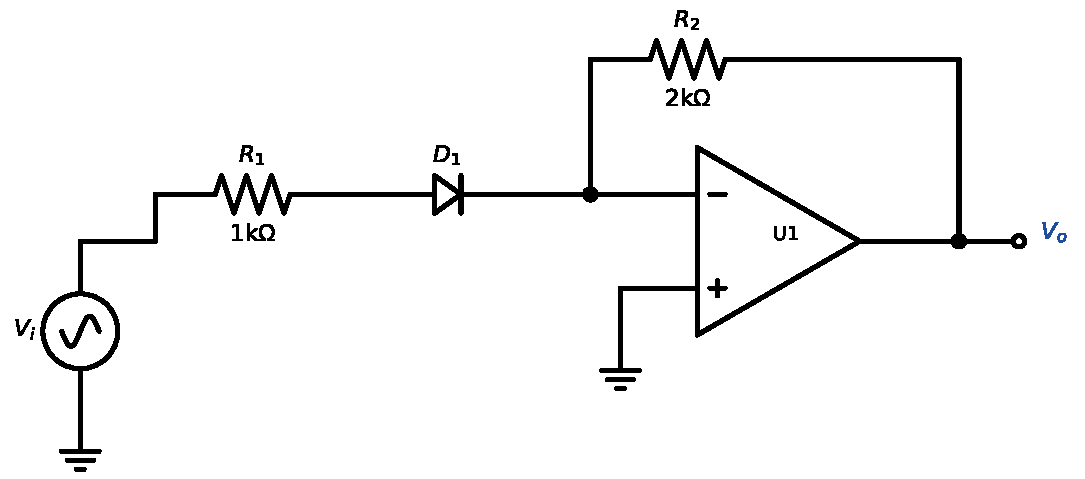
\includegraphics[width=\linewidth,height=5.6cm,keepaspectratio]{p05_circuit}\end{center}
\end{probbox}

\begin{probbox}{Problem 3B.6 \hfill Easy}
For the circuit below (ideal op-amps), use the ideal-diode model. Find $V_o$ as a function of $V_i$ and sketch $V_o$ versus $V_i$. Also sketch $V_o(t)$ for $V_i(t) = 2\sin(2\pi\cdot 1000\,t)$.
\begin{center}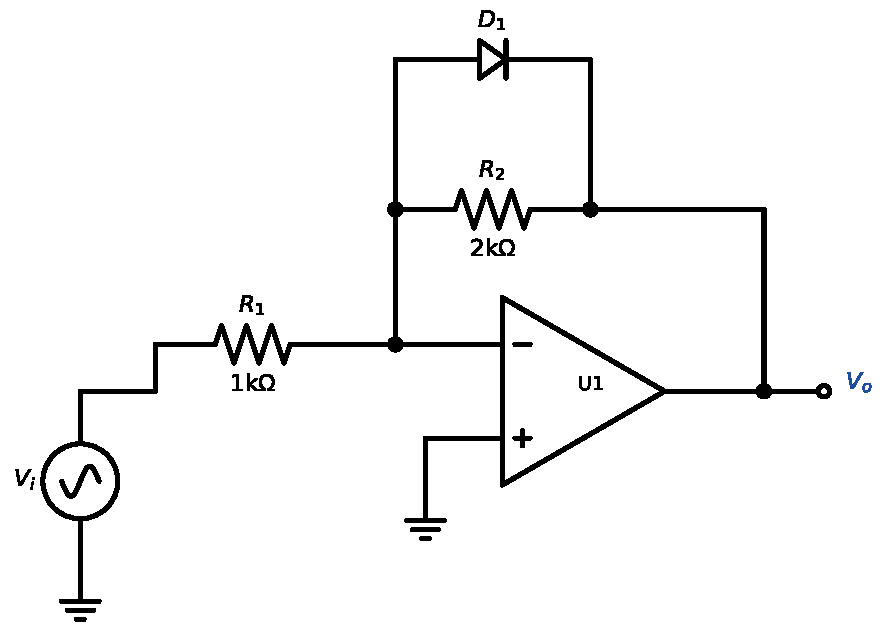
\includegraphics[width=\linewidth,height=5.6cm,keepaspectratio]{p06_circuit}\end{center}
\end{probbox}

\subsection*{Medium problems}
\begin{probbox}{Problem 3B.7 \hfill Medium}
For the circuit below (ideal op-amps), use the constant-voltage-drop model ($V_{D,on}=0.7$\,V). Find $V_o$ as a function of $V_i$ and sketch $V_o$ versus $V_i$. Also sketch $V_o(t)$ for $V_i(t) = 0.5\sin(2\pi\cdot 1000\,t)$.
\begin{center}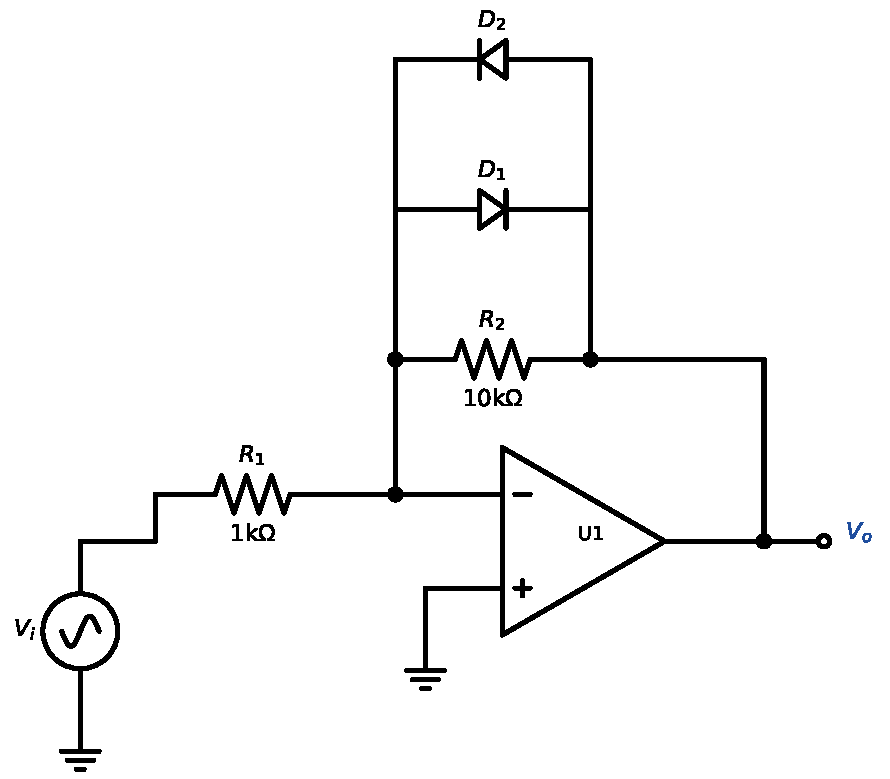
\includegraphics[width=\linewidth,height=5.6cm,keepaspectratio]{p07_circuit}\end{center}
\end{probbox}

\begin{probbox}{Problem 3B.8 \hfill Medium}
For the circuit below (ideal op-amps), use the constant-voltage-drop model ($V_{D,on}=0.7$\,V). Find $V_o$ as a function of $V_i$ and sketch $V_o$ versus $V_i$. Also sketch $V_o(t)$ for $V_i(t) = 2\sin(2\pi\cdot 500\,t)$.
\begin{center}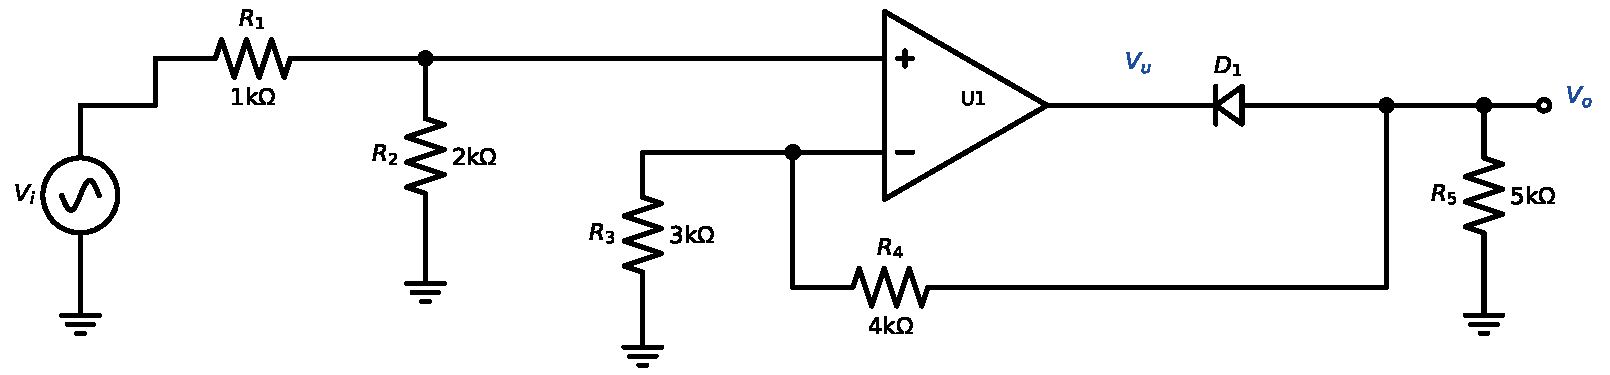
\includegraphics[width=\linewidth,height=5.6cm,keepaspectratio]{p08_circuit}\end{center}
\end{probbox}

\begin{probbox}{Problem 3B.9 \hfill Medium}
For the circuit below (ideal op-amps), use the constant-voltage-drop model ($V_{D,on}=0.7$\,V). Find $V_o$ as a function of $V_i$ and sketch $V_o$ versus $V_i$. Also sketch $V_o(t)$ for $V_i(t) = 1\sin(2\pi\cdot 1000\,t)$.
\begin{center}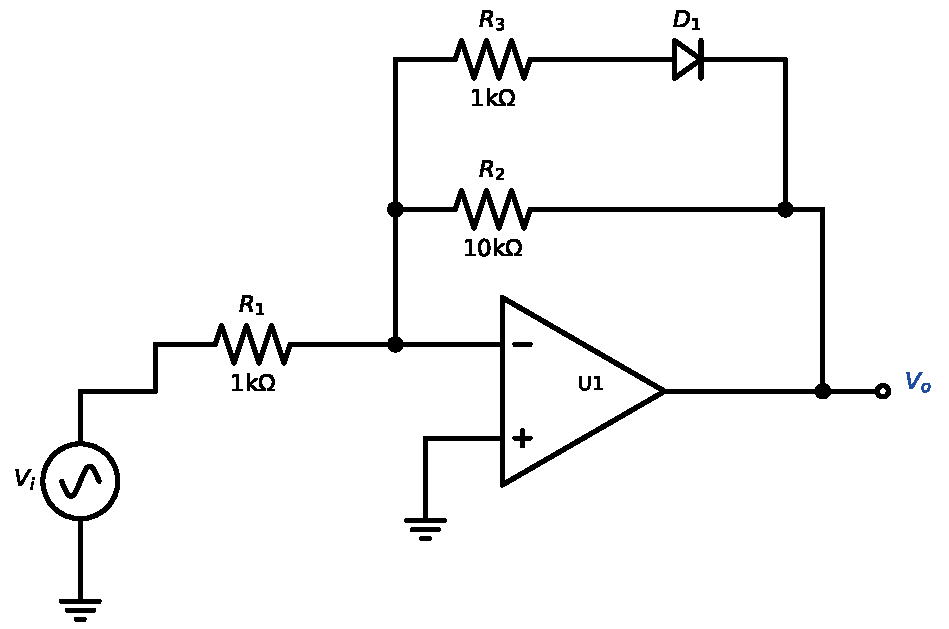
\includegraphics[width=\linewidth,height=5.6cm,keepaspectratio]{p09_circuit}\end{center}
\end{probbox}

\begin{probbox}{Problem 3B.10 \hfill Medium}
For the circuit below (ideal op-amps), use the constant-voltage-drop model ($V_{D,on}=0.7$\,V). Find $V_o$ as a function of $V_i$ and sketch $V_o$ versus $V_i$. Also sketch $V_o(t)$ for $V_i(t) = 1\sin(2\pi\cdot 1000\,t)$.
\begin{center}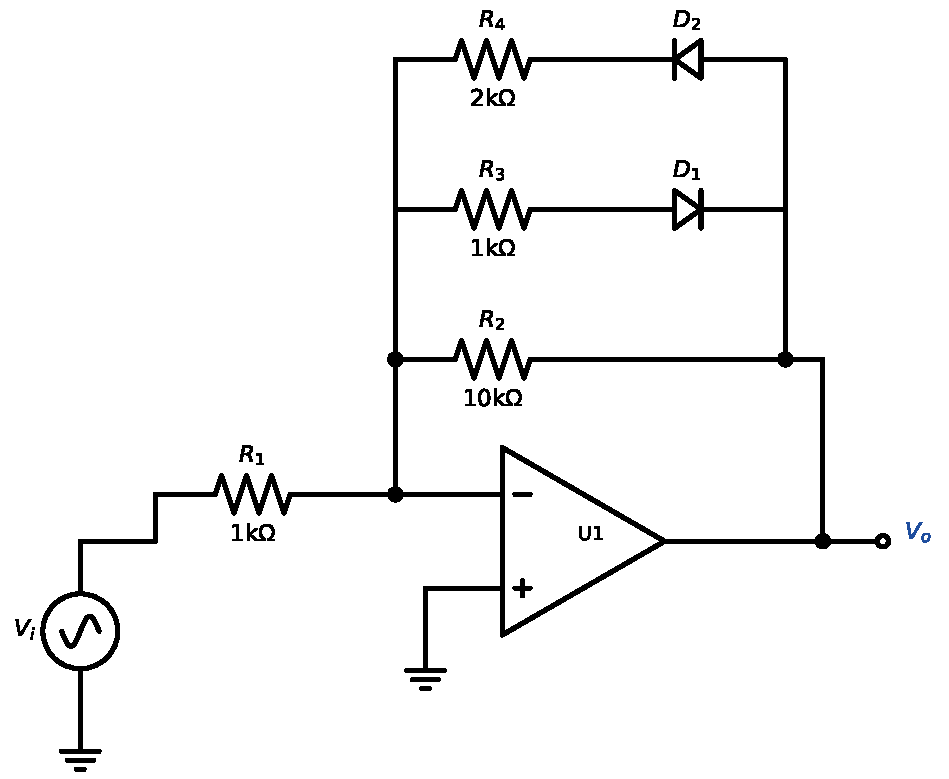
\includegraphics[width=\linewidth,height=5.6cm,keepaspectratio]{p10_circuit}\end{center}
\end{probbox}

\begin{probbox}{Problem 3B.11 \hfill Medium}
For the circuit below (ideal op-amps), use the constant-voltage-drop model ($V_{D,on}=0.7$\,V). Find $V_o$ as a function of $V_i$ and sketch $V_o$ versus $V_i$. Also sketch $V_o(t)$ for $V_i(t) = 4\sin(2\pi\cdot 1000\,t)$.
\begin{center}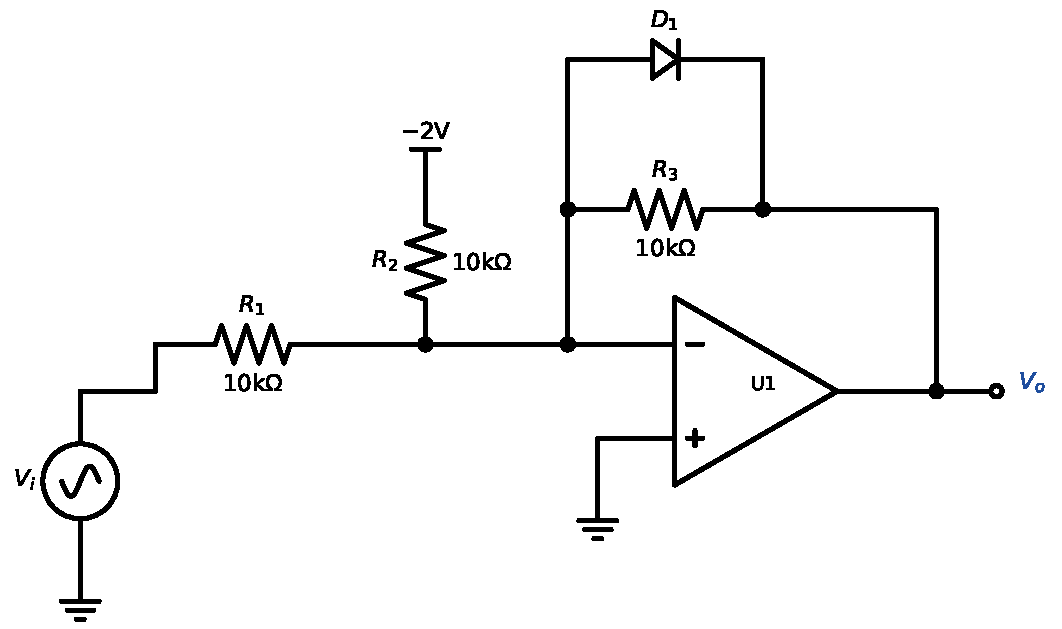
\includegraphics[width=\linewidth,height=5.6cm,keepaspectratio]{p11_circuit}\end{center}
\end{probbox}

\begin{probbox}{Problem 3B.12 \hfill Medium}
For the circuit below (ideal op-amps), use the constant-voltage-drop model ($V_{D,on}=0.7$\,V). Find $V_o$ as a function of $V_i$ and sketch $V_o$ versus $V_i$. Also sketch $V_o(t)$ for $V_i(t) = 1\sin(2\pi\cdot 1000\,t)$.
\begin{center}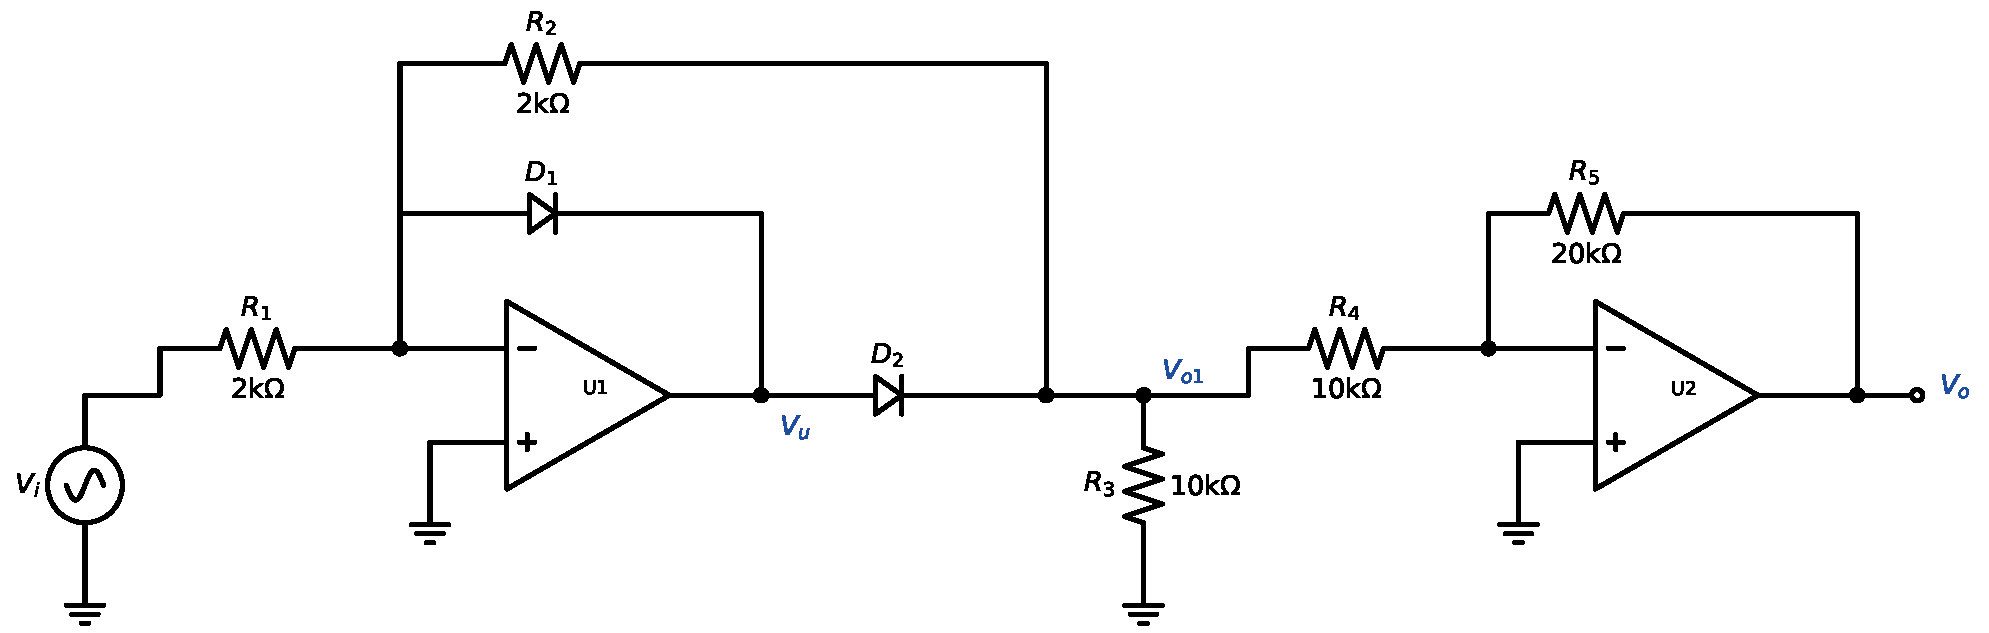
\includegraphics[width=\linewidth,height=5.6cm,keepaspectratio]{p12_circuit}\end{center}
\end{probbox}

\subsection*{Hard problems}
\begin{probbox}{Problem 3B.13 \hfill Hard}
For the circuit below (ideal op-amps), use the constant-voltage-drop model ($V_{D,on}=0.7$\,V). Find $V_o$ as a function of $V_i$ and sketch $V_o$ versus $V_i$. Also sketch $V_o(t)$ for $V_i(t) = 0.3\sin(2\pi\cdot 1000\,t)$.
\begin{center}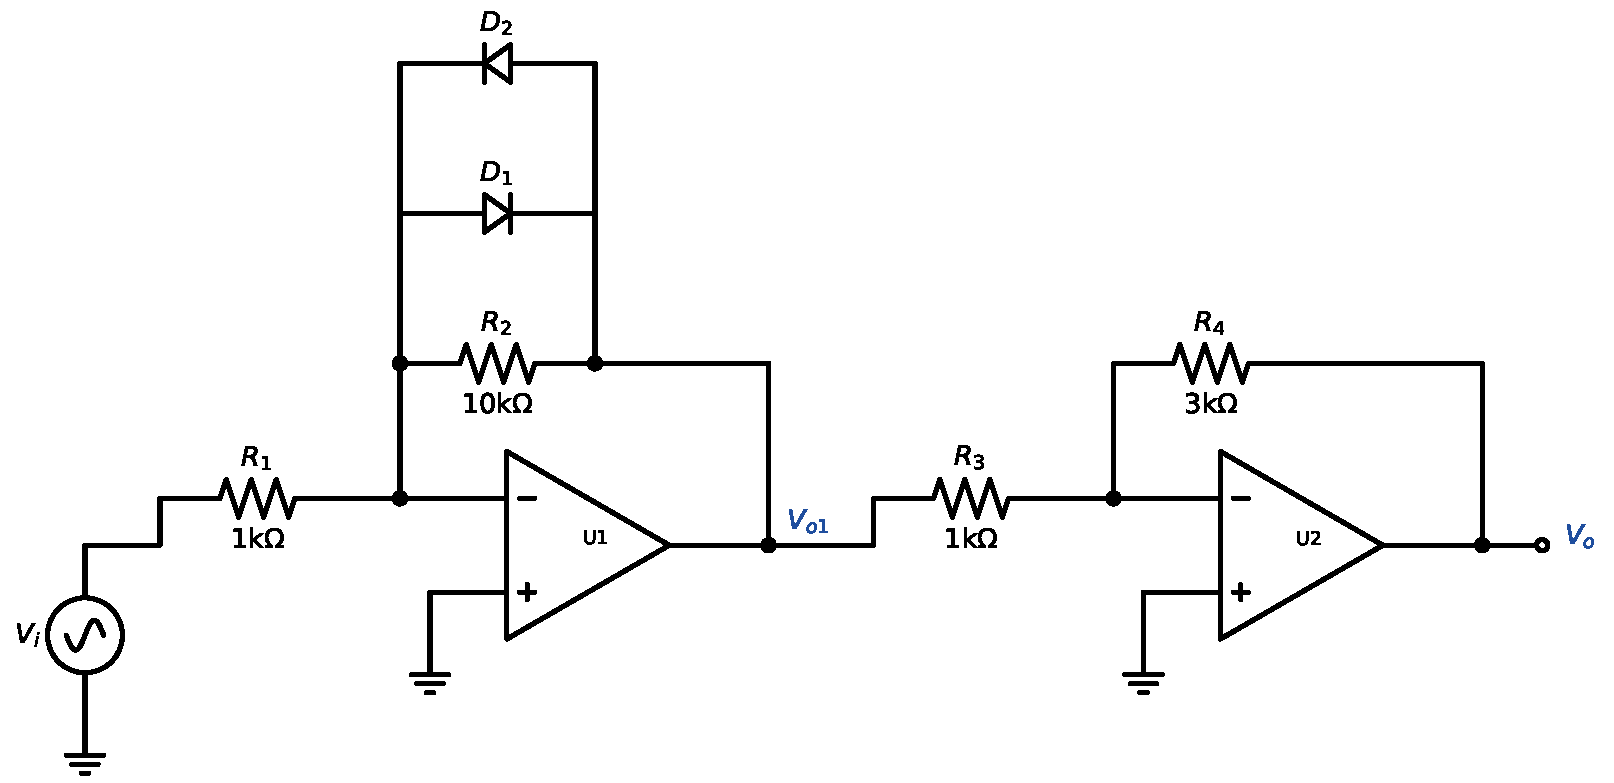
\includegraphics[width=\linewidth,height=5.6cm,keepaspectratio]{p13_circuit}\end{center}
\end{probbox}

\begin{probbox}{Problem 3B.14 \hfill Hard}
For the circuit below (ideal op-amps), use the constant-voltage-drop model ($V_{D,on}=0.7$\,V). Find $V_o$ as a function of $V_i$ and sketch $V_o$ versus $V_i$. Also sketch $V_o(t)$ for $V_i(t) = 1\sin(2\pi\cdot 500\,t)$.
\begin{center}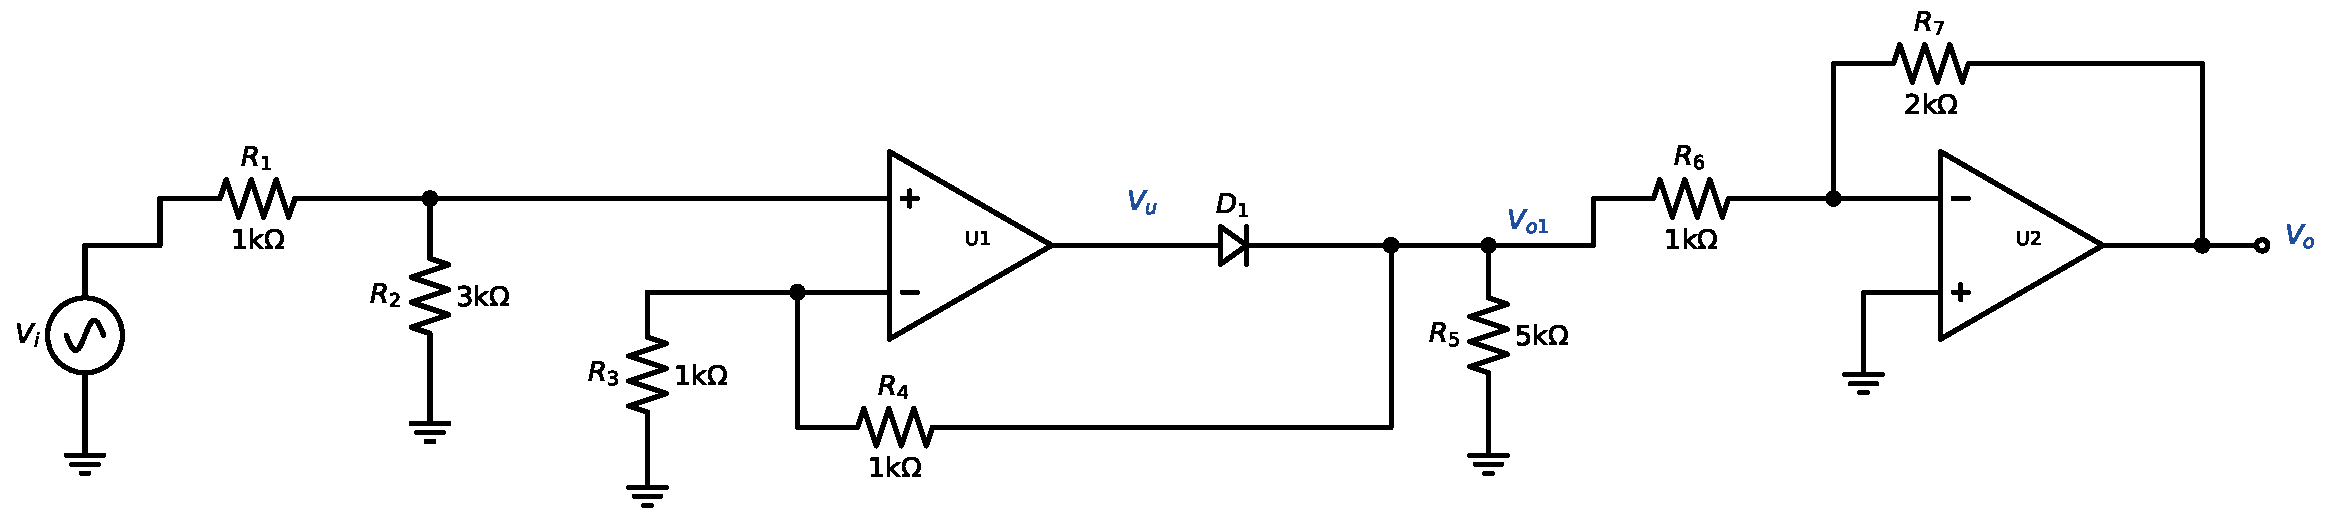
\includegraphics[width=\linewidth,height=5.6cm,keepaspectratio]{p14_circuit}\end{center}
\end{probbox}

\begin{probbox}{Problem 3B.15 \hfill Hard}
For the circuit below (ideal op-amps), use the constant-voltage-drop model ($V_{D,on}=0.7$\,V). Find $V_o$ as a function of $V_i$ and sketch $V_o$ versus $V_i$. Also sketch $V_o(t)$ for $V_i(t) = 1\sin(2\pi\cdot 1000\,t)$.
\begin{center}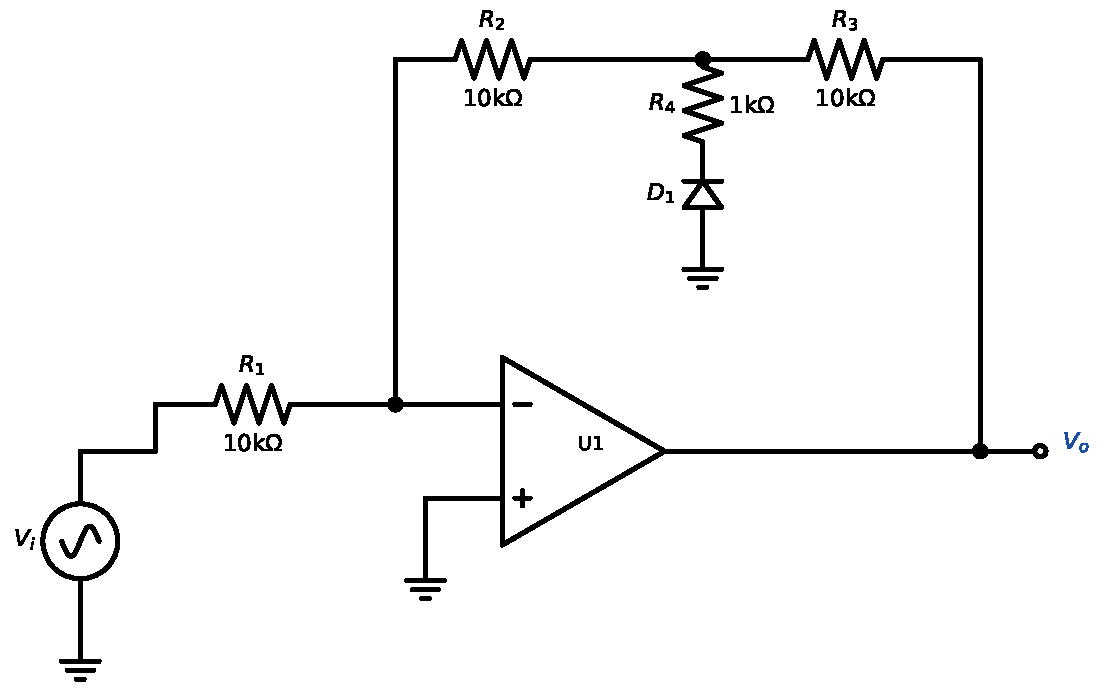
\includegraphics[width=\linewidth,height=5.6cm,keepaspectratio]{p15_circuit}\end{center}
\end{probbox}

\begin{probbox}{Problem 3B.16 \hfill Hard}
For the circuit below (ideal op-amps), use the constant-voltage-drop model ($V_{D,on}=0.7$\,V). Find $V_o$ as a function of $V_i$ and sketch $V_o$ versus $V_i$. Also sketch $V_o(t)$ for $V_i(t) = 2\sin(2\pi\cdot 1000\,t)$.
\begin{center}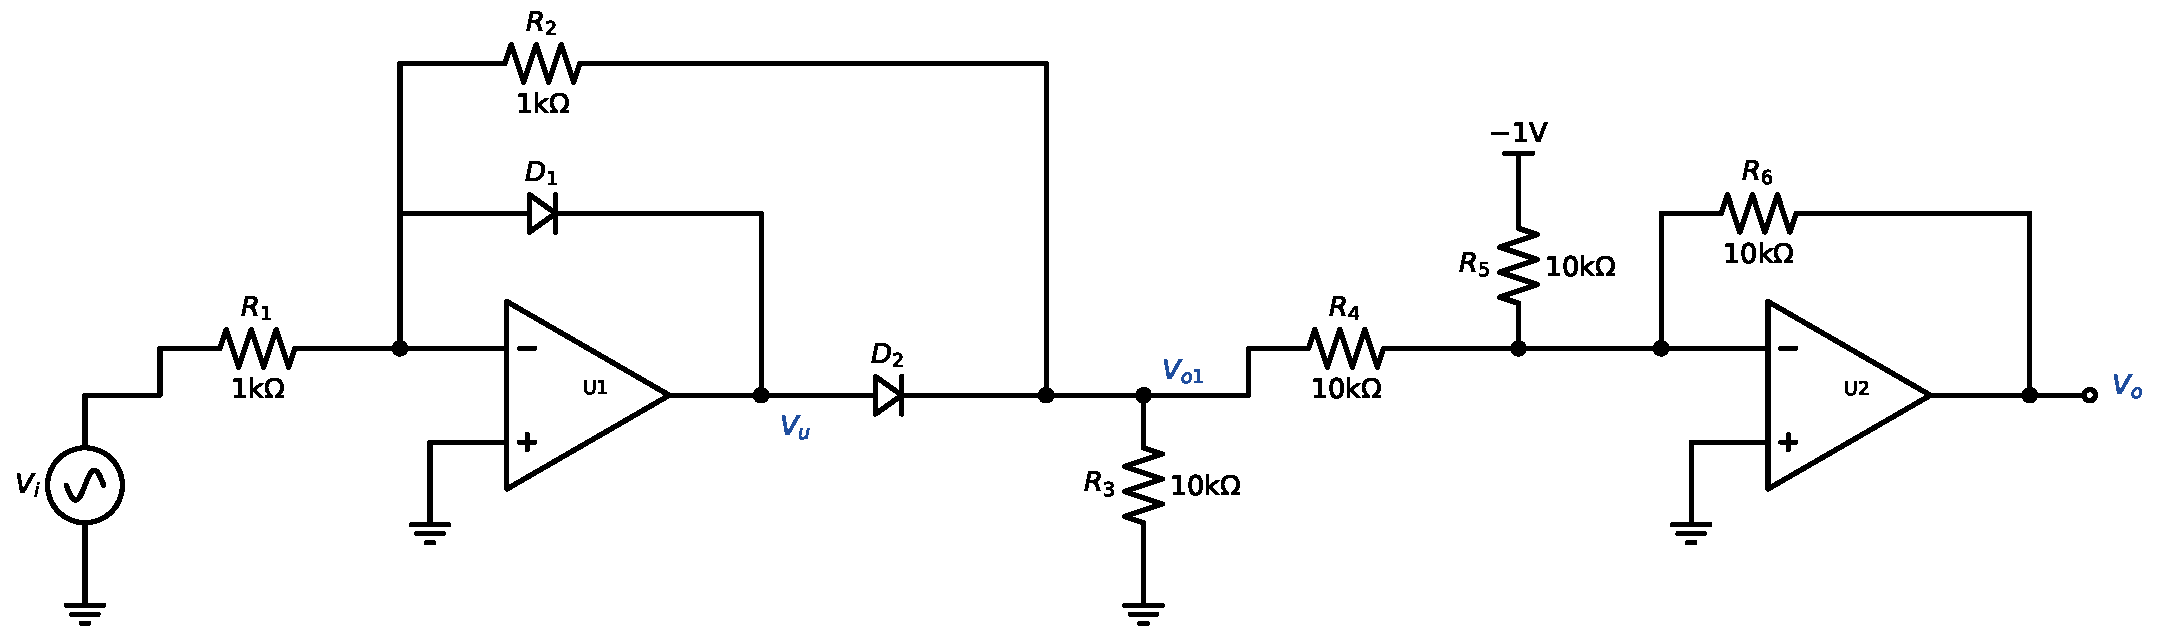
\includegraphics[width=\linewidth,height=5.6cm,keepaspectratio]{p16_circuit}\end{center}
\end{probbox}

\begin{probbox}{Problem 3B.17 \hfill Hard}
For the circuit below (ideal op-amps), use the constant-voltage-drop model ($V_{D,on}=0.7$\,V). Find $V_o$ as a function of $V_i$ and sketch $V_o$ versus $V_i$. Also sketch $V_o(t)$ for $V_i(t) = 2\sin(2\pi\cdot 1000\,t)$.
\begin{center}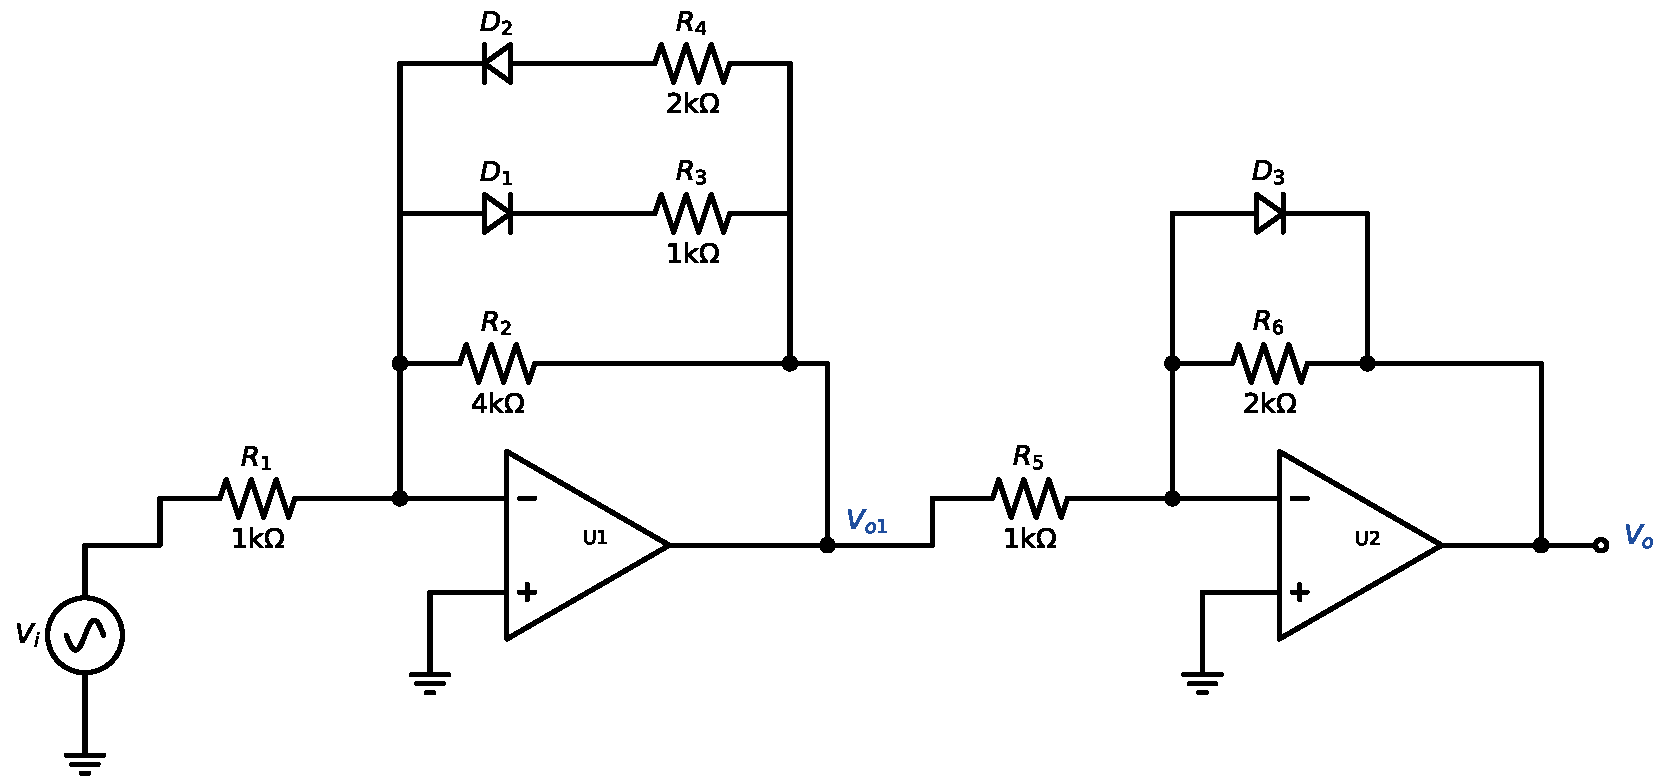
\includegraphics[width=\linewidth,height=5.6cm,keepaspectratio]{p17_circuit}\end{center}
\end{probbox}

\begin{probbox}{Problem 3B.18 \hfill Hard}
For the circuit below (ideal op-amps), use the constant-voltage-drop model ($V_{D,on}=0.7$\,V). Find $V_o$ as a function of $V_i$ and sketch $V_o$ versus $V_i$. Also sketch $V_o(t)$ for $V_i(t) = 3\sin(2\pi\cdot 1000\,t)$.
\begin{center}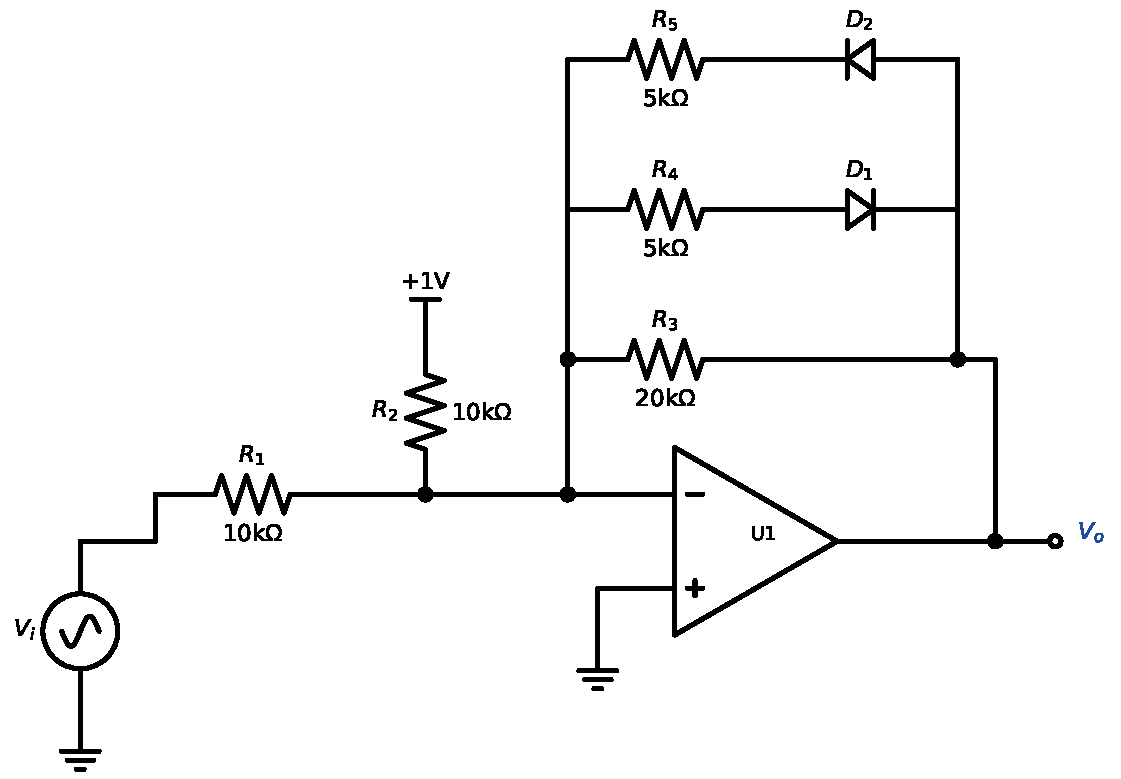
\includegraphics[width=\linewidth,height=5.6cm,keepaspectratio]{p18_circuit}\end{center}
\end{probbox}

\newpage
\section*{Solutions}
Every solution follows the steps of the Lecture-3 pipeline card.
\newpage
\subsection*{Solution 3B.1 \hfill Easy}
\begin{center}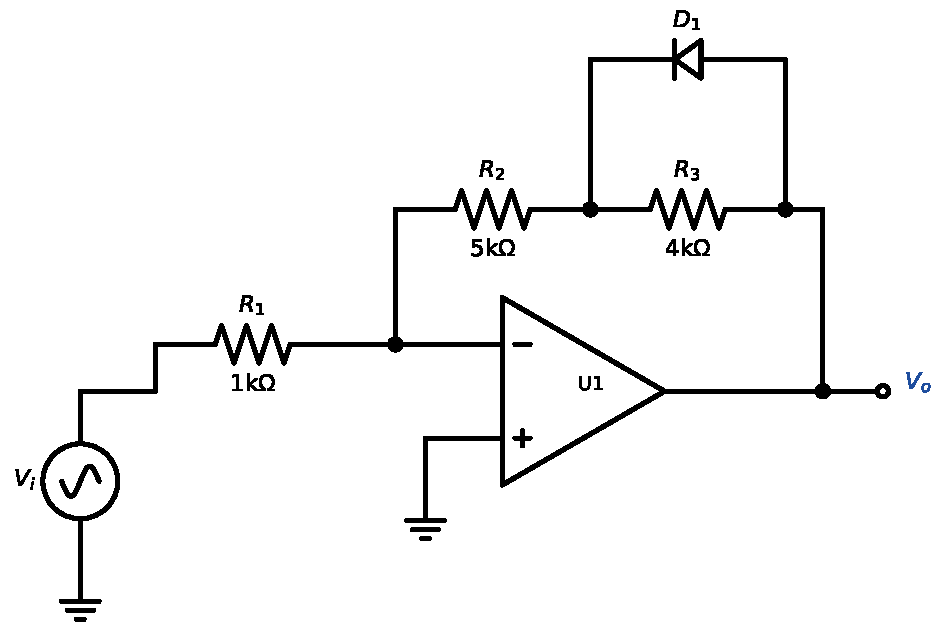
\includegraphics[width=0.9\linewidth,height=5cm,keepaspectratio]{p01_circuit}\end{center}
\solstep{1}{Model and method}Use the constant-voltage-drop model (tool T1): an OFF diode is an open circuit and needs $V_D<0.7$\,V; an ON diode is a $0.7$\,V source and needs $I_D>0$. With 1 diode there are $2$ ON/OFF combinations. For each one the circuit is linear: solve it with $V_i$ kept as a symbol, then check its assumptions --- each check is a condition on $V_i$ (tool T2). Op-amps are ideal ($A\to\infty$). Whether an op-amp has negative feedback can depend on the diode states, so decide it separately for every combination. Node names used below: $V_{-}$ = the op-amp's $-$ input; $V_{a}$ = node joining $D_{1}, R_{2}, R_{3}$.
\solstep{2}{Assume $D_{1}$ ON}Replace $D_{1}$ ON: a $0.7$\,V source ($V_{o} - V_{a} = 0.7$) carrying an unknown current $I_{D_{1}}$ from anode to cathode. U1 has negative feedback, so $V_- = V_+$ (virtual short) and no current flows into its inputs.

Equations (KCL at every node that is not an op-amp output, plus the diode voltages):\begin{align*}
&\text{KCL at }V_{-}\,(=0): && \frac{0 - V_i}{R_{1}} + \frac{0 - V_{a}}{R_{2}} = 0 \\
&\text{KCL at }V_{a}: && \frac{V_{a}}{R_{2}} + \frac{V_{a} - V_{o}}{R_{3}} - I_{D_{1}} = 0 \\
&\text{D1 ON}: && V_{o} - V_{a} = 0.7
\end{align*}


Solving these linear equations (substitute one into the other, as in Lecture 2) gives, with $V_i$ kept as a symbol:\begin{align*}
V_{o} &= -5V_i + 0.7 \\
I_{D_{1}} &= -V_i - 0.175\ \mathrm{mA}
\end{align*}


Check the assumptions: $I_{D_{1}} > 0$ $\Rightarrow$ $V_i < -0.175$\,V. So this state holds for $\boxed{V_i < -0.175}$, where $V_o = -5V_i + 0.7$.
\solstep{3}{Assume $D_{1}$ OFF}Replace $D_{1}$ OFF: an open circuit. U1 has negative feedback, so $V_- = V_+$ (virtual short) and no current flows into its inputs.

Equations (KCL at every node that is not an op-amp output, plus the diode voltages):\begin{align*}
&\text{KCL at }V_{-}\,(=0): && \frac{0 - V_i}{R_{1}} + \frac{0 - V_{a}}{R_{2}} = 0 \\
&\text{KCL at }V_{a}: && \frac{V_{a}}{R_{2}} + \frac{V_{a} - V_{o}}{R_{3}} = 0
\end{align*}


Solving these linear equations (substitute one into the other, as in Lecture 2) gives, with $V_i$ kept as a symbol:\begin{align*}
V_{o} &= -9V_i \\
V_{D_{1}} = V_{o} - V_{a} &= -4V_i
\end{align*}


Check the assumptions: $V_{D_{1}} < 0.7$ $\Rightarrow$ $V_i > -0.175$\,V. So this state holds for $\boxed{V_i > -0.175}$, where $V_o = -9V_i$.
\solstep{4}{Assemble and sketch}Put the valid states together:\[
V_o = \begin{cases} -5V_i + 0.7 & V_i < -0.175 \\ -9V_i & V_i > -0.175 \end{cases}
\]
Check: the pieces must meet at each breakpoint --- at $V_i=-0.175$\,V both pieces give $V_o=1.575$\,V. \checkmark\begin{center}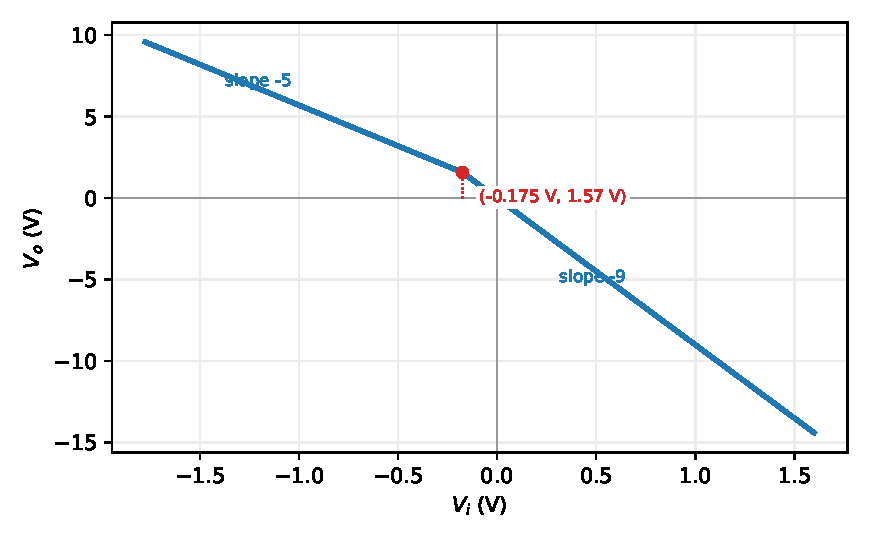
\includegraphics[width=0.62\linewidth,height=6cm,keepaspectratio]{p01_transfer}\end{center}

\begin{ansbox}
$V_o = \begin{cases} -5V_i + 0.7 & V_i < -0.175 \\ -9V_i & V_i > -0.175 \end{cases}$
\end{ansbox}

\newpage
\subsection*{Solution 3B.2 \hfill Easy}
\begin{center}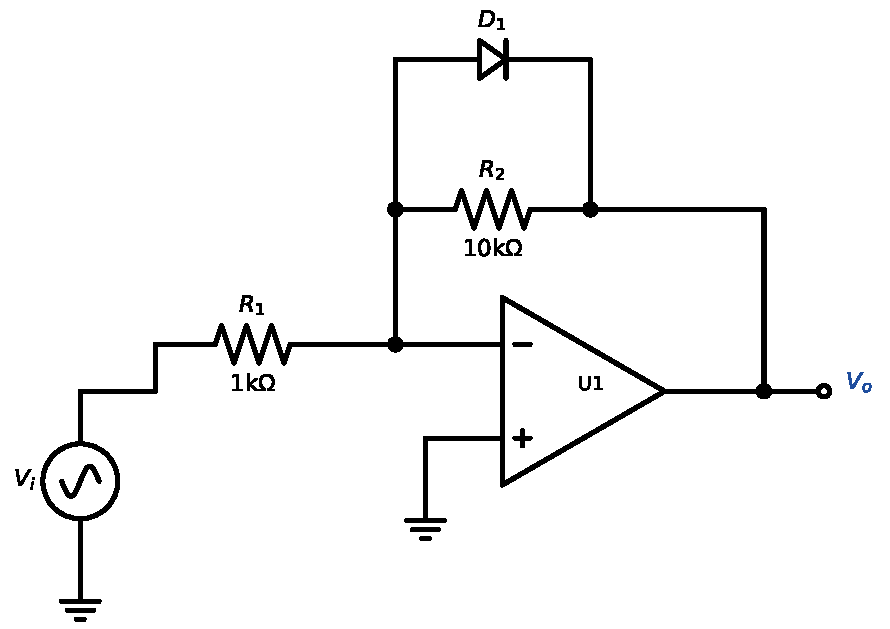
\includegraphics[width=0.9\linewidth,height=5cm,keepaspectratio]{p02_circuit}\end{center}
\solstep{1}{Model and method}Use the constant-voltage-drop model (tool T1): an OFF diode is an open circuit and needs $V_D<0.7$\,V; an ON diode is a $0.7$\,V source and needs $I_D>0$. With 1 diode there are $2$ ON/OFF combinations. For each one the circuit is linear: solve it with $V_i$ kept as a symbol, then check its assumptions --- each check is a condition on $V_i$ (tool T2). Op-amps are ideal ($A\to\infty$). Whether an op-amp has negative feedback can depend on the diode states, so decide it separately for every combination. Node names used below: $V_{-}$ = the op-amp's $-$ input.
\solstep{2}{Assume $D_{1}$ OFF}Replace $D_{1}$ OFF: an open circuit. U1 has negative feedback, so $V_- = V_+$ (virtual short) and no current flows into its inputs.

Equations (KCL at every node that is not an op-amp output, plus the diode voltages):\begin{align*}
&\text{KCL at }V_{-}\,(=0): && \frac{0 - V_i}{R_{1}} + \frac{0 - V_{o}}{R_{2}} = 0
\end{align*}


Solving these linear equations (substitute one into the other, as in Lecture 2) gives, with $V_i$ kept as a symbol:\begin{align*}
V_{o} &= -10V_i \\
V_{D_{1}} = V_{-} - V_{o} &= 10V_i
\end{align*}


Check the assumptions: $V_{D_{1}} < 0.7$ $\Rightarrow$ $V_i < 0.07$\,V. So this state holds for $\boxed{V_i < 0.07}$, where $V_o = -10V_i$.
\solstep{3}{Assume $D_{1}$ ON}Replace $D_{1}$ ON: a $0.7$\,V source ($V_{-} - V_{o} = 0.7$) carrying an unknown current $I_{D_{1}}$ from anode to cathode. U1 has negative feedback, so $V_- = V_+$ (virtual short) and no current flows into its inputs.

Equations (KCL at every node that is not an op-amp output, plus the diode voltages):\begin{align*}
&\text{KCL at }V_{-}\,(=0): && \frac{0 - V_i}{R_{1}} + \frac{0 - V_{o}}{R_{2}} + I_{D_{1}} = 0 \\
&\text{D1 ON}: && 0 - V_{o} = 0.7
\end{align*}


Solving these linear equations (substitute one into the other, as in Lecture 2) gives, with $V_i$ kept as a symbol:\begin{align*}
V_{o} &= -0.7 \\
I_{D_{1}} &= V_i - 0.07\ \mathrm{mA}
\end{align*}


Check the assumptions: $I_{D_{1}} > 0$ $\Rightarrow$ $V_i > 0.07$\,V. So this state holds for $\boxed{V_i > 0.07}$, where $V_o = -0.7$.
\solstep{4}{Assemble and sketch}Put the valid states together:\[
V_o = \begin{cases} -10V_i & V_i < 0.07 \\ -0.7 & V_i > 0.07 \end{cases}
\]
Check: the pieces must meet at each breakpoint --- at $V_i=0.07$\,V both pieces give $V_o=-0.7$\,V. \checkmark\begin{center}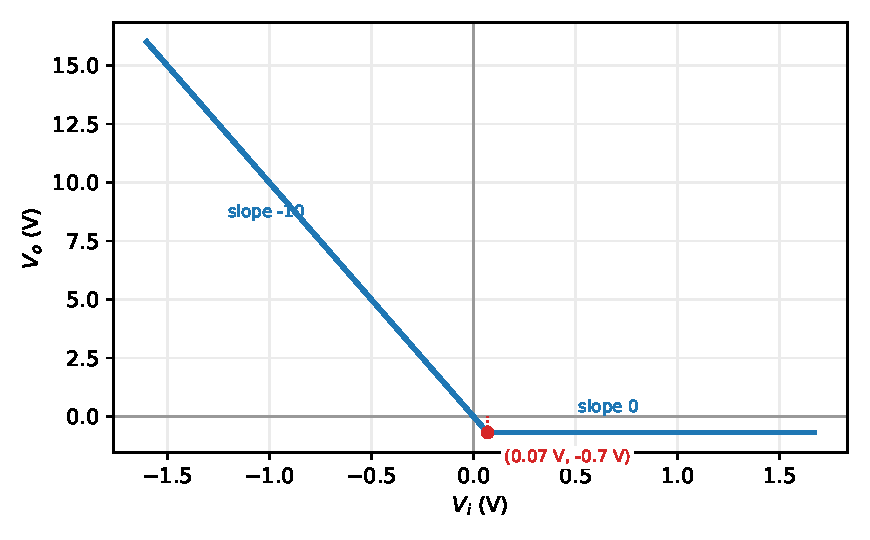
\includegraphics[width=0.62\linewidth,height=6cm,keepaspectratio]{p02_transfer}\end{center}
For $V_i(t) = 1\sin(2\pi\cdot 1000\,t)$ simply pass every instant of $V_i(t)$ through the characteristic above (each piece is a straight line, so each part of the sinusoid is scaled and shifted):\begin{center}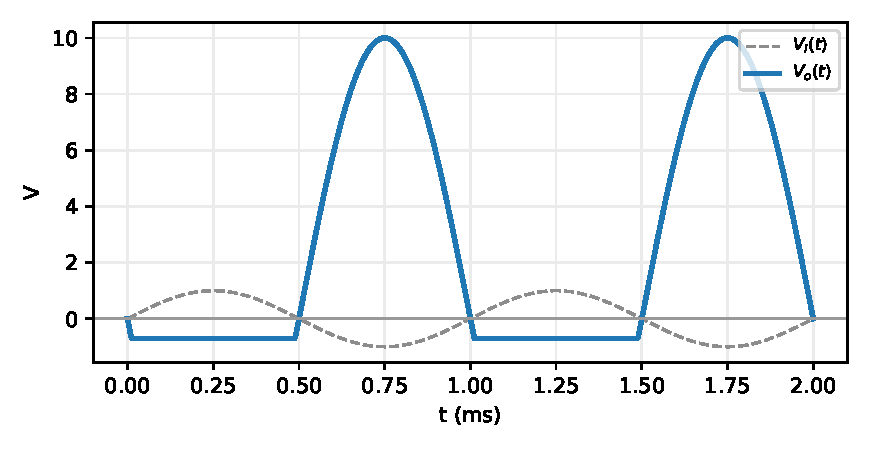
\includegraphics[width=0.62\linewidth,height=5cm,keepaspectratio]{p02_time}\end{center}

\begin{ansbox}
$V_o = \begin{cases} -10V_i & V_i < 0.07 \\ -0.7 & V_i > 0.07 \end{cases}$
\end{ansbox}

\newpage
\subsection*{Solution 3B.3 \hfill Easy}
\begin{center}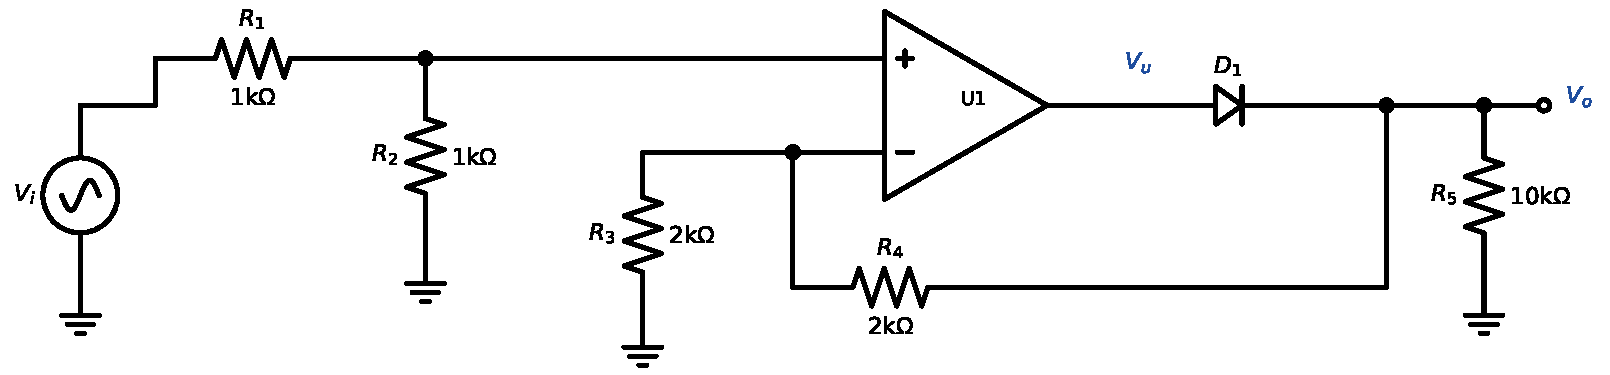
\includegraphics[width=0.9\linewidth,height=5cm,keepaspectratio]{p03_circuit}\end{center}
\solstep{1}{Model and method}Use the constant-voltage-drop model (tool T1): an OFF diode is an open circuit and needs $V_D<0.7$\,V; an ON diode is a $0.7$\,V source and needs $I_D>0$. With 1 diode there are $2$ ON/OFF combinations. For each one the circuit is linear: solve it with $V_i$ kept as a symbol, then check its assumptions --- each check is a condition on $V_i$ (tool T2). Op-amps are ideal ($A\to\infty$). Whether an op-amp has negative feedback can depend on the diode states, so decide it separately for every combination. Node names used below: $V_{+}$ = the op-amp's $+$ input; $V_{-}$ = the op-amp's $-$ input.
\solstep{2}{Assume $D_{1}$ OFF}Replace $D_{1}$ OFF: an open circuit. With this assumption U1 has no feedback path from its output back to its $-$ input: it runs \emph{open-loop}, $V_{u} = A(V_+ - V_-)$ with $A\to\infty$, so its output is pushed to $\pm\infty$ (in practice, a supply rail) unless $V_+ = V_-$ exactly.

Equations (KCL at every node that is not an op-amp output, plus the diode voltages):\begin{align*}
&\text{KCL at }V_{+}: && \frac{V_{+} - V_i}{R_{1}} + \frac{V_{+}}{R_{2}} = 0 \\
&\text{KCL at }V_{-}: && \frac{V_{-}}{R_{3}} + \frac{V_{-} - V_{o}}{R_{4}} = 0 \\
&\text{KCL at }V_{o}: && \frac{V_{o} - V_{-}}{R_{4}} + \frac{V_{o}}{R_{5}} = 0
\end{align*}


Solving these linear equations (substitute one into the other, as in Lecture 2) gives, with $V_i$ kept as a symbol:\begin{align*}
V_{o} &= 0 \\
V_{D_{1}} = V_{u} - V_{o} &\approx A\left(0.5V_i\right)
\end{align*}


Check the assumptions: $V_{D_{1}} < 0.7$; since $A\to\infty$ this needs $0.5V_i < 0$ $\Rightarrow$ $V_i < 0$\,V. So this state holds for $\boxed{V_i < 0}$, where $V_o = 0$.
\solstep{3}{Assume $D_{1}$ ON}Replace $D_{1}$ ON: a $0.7$\,V source ($V_{u} - V_{o} = 0.7$) carrying an unknown current $I_{D_{1}}$ from anode to cathode. U1 has negative feedback, so $V_- = V_+$ (virtual short) and no current flows into its inputs.

Equations (KCL at every node that is not an op-amp output, plus the diode voltages):\begin{align*}
&\text{KCL at }V_{+}: && \frac{V_{+} - V_i}{R_{1}} + \frac{V_{+}}{R_{2}} = 0 \\
&\text{KCL at }V_{-}\,(=V_{+}): && \frac{V_{+}}{R_{3}} + \frac{V_{+} - V_{o}}{R_{4}} = 0 \\
&\text{KCL at }V_{o}: && \frac{V_{o} - V_{+}}{R_{4}} + \frac{V_{o}}{R_{5}} - I_{D_{1}} = 0 \\
&\text{D1 ON}: && V_{u} - V_{o} = 0.7
\end{align*}


Solving these linear equations (substitute one into the other, as in Lecture 2) gives, with $V_i$ kept as a symbol:\begin{align*}
V_{o} &= V_i \\
I_{D_{1}} &= 0.35V_i\ \mathrm{mA}
\end{align*}


Check the assumptions: $I_{D_{1}} > 0$ $\Rightarrow$ $V_i > 0$\,V. So this state holds for $\boxed{V_i > 0}$, where $V_o = V_i$.
\solstep{4}{Assemble and sketch}Put the valid states together:\[
V_o = \begin{cases} 0 & V_i < 0 \\ V_i & V_i > 0 \end{cases}
\]
Check: the pieces must meet at each breakpoint --- at $V_i=0$\,V both pieces give $V_o=0$\,V. \checkmark\begin{center}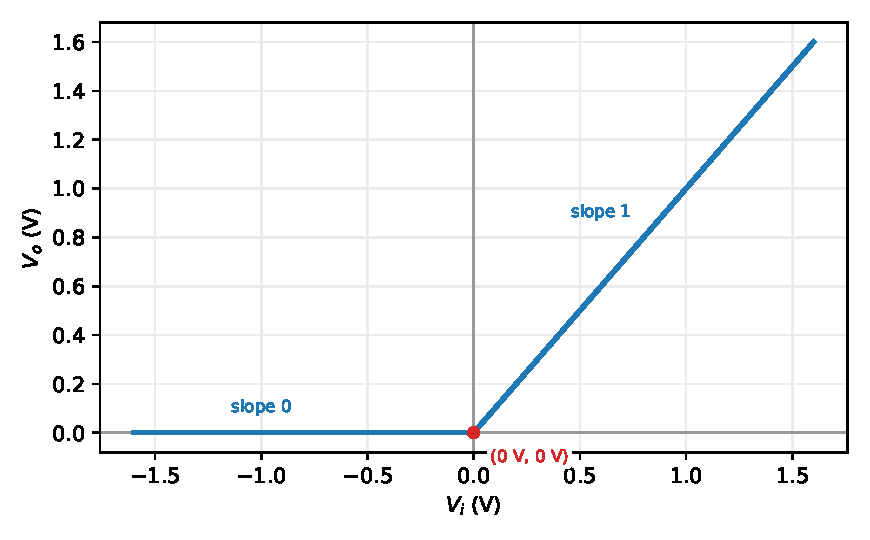
\includegraphics[width=0.62\linewidth,height=6cm,keepaspectratio]{p03_transfer}\end{center}
For $V_i(t) = 2\sin(2\pi\cdot 500\,t)$ simply pass every instant of $V_i(t)$ through the characteristic above (each piece is a straight line, so each part of the sinusoid is scaled and shifted):\begin{center}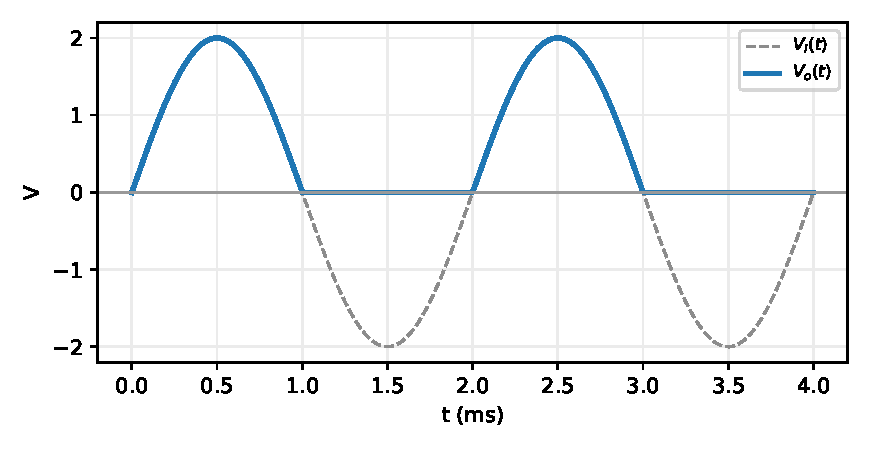
\includegraphics[width=0.62\linewidth,height=5cm,keepaspectratio]{p03_time}\end{center}

\begin{ansbox}
$V_o = \begin{cases} 0 & V_i < 0 \\ V_i & V_i > 0 \end{cases}$
\end{ansbox}

\newpage
\subsection*{Solution 3B.4 \hfill Easy}
\begin{center}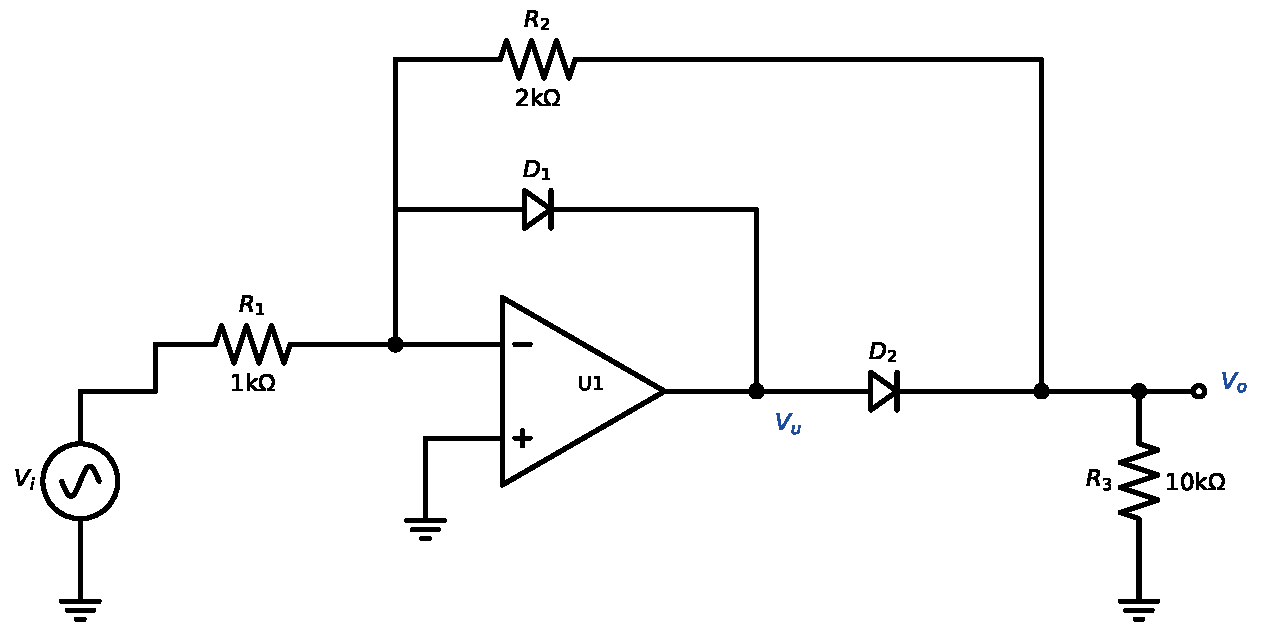
\includegraphics[width=0.9\linewidth,height=5cm,keepaspectratio]{p04_circuit}\end{center}
\solstep{1}{Model and method}Use the constant-voltage-drop model (tool T1): an OFF diode is an open circuit and needs $V_D<0.7$\,V; an ON diode is a $0.7$\,V source and needs $I_D>0$. With 2 diodes there are $4$ ON/OFF combinations. For each one the circuit is linear: solve it with $V_i$ kept as a symbol, then check its assumptions --- each check is a condition on $V_i$ (tool T2). Op-amps are ideal ($A\to\infty$). Whether an op-amp has negative feedback can depend on the diode states, so decide it separately for every combination. Node names used below: $V_{-}$ = the op-amp's $-$ input.
\solstep{2}{Assume $D_{1}$ OFF, $D_{2}$ ON}Replace $D_{1}$ OFF: an open circuit; $D_{2}$ ON: a $0.7$\,V source ($V_{u} - V_{o} = 0.7$) carrying an unknown current $I_{D_{2}}$ from anode to cathode. U1 has negative feedback, so $V_- = V_+$ (virtual short) and no current flows into its inputs.

Equations (KCL at every node that is not an op-amp output, plus the diode voltages):\begin{align*}
&\text{KCL at }V_{-}\,(=0): && \frac{0 - V_i}{R_{1}} + \frac{0 - V_{o}}{R_{2}} = 0 \\
&\text{KCL at }V_{o}: && \frac{V_{o}}{R_{2}} + \frac{V_{o}}{R_{3}} - I_{D_{2}} = 0 \\
&\text{D2 ON}: && V_{u} - V_{o} = 0.7
\end{align*}


Solving these linear equations (substitute one into the other, as in Lecture 2) gives, with $V_i$ kept as a symbol:\begin{align*}
V_{o} &= -2V_i \\
V_{D_{1}} = V_{-} - V_{u} &= 2V_i - 0.7 \\
I_{D_{2}} &= -1.2V_i\ \mathrm{mA}
\end{align*}


Check the assumptions: $V_{D_{1}} < 0.7$ $\Rightarrow$ $V_i < 0.7$\,V; $I_{D_{2}} > 0$ $\Rightarrow$ $V_i < 0$\,V. So this state holds for $\boxed{V_i < 0}$, where $V_o = -2V_i$.
\solstep{3}{Assume $D_{1}$ ON, $D_{2}$ OFF}Replace $D_{1}$ ON: a $0.7$\,V source ($V_{-} - V_{u} = 0.7$) carrying an unknown current $I_{D_{1}}$ from anode to cathode; $D_{2}$ OFF: an open circuit. U1 has negative feedback, so $V_- = V_+$ (virtual short) and no current flows into its inputs.

Equations (KCL at every node that is not an op-amp output, plus the diode voltages):\begin{align*}
&\text{KCL at }V_{-}\,(=0): && \frac{0 - V_i}{R_{1}} + \frac{0 - V_{o}}{R_{2}} + I_{D_{1}} = 0 \\
&\text{KCL at }V_{o}: && \frac{V_{o}}{R_{2}} + \frac{V_{o}}{R_{3}} = 0 \\
&\text{D1 ON}: && 0 - V_{u} = 0.7
\end{align*}


Solving these linear equations (substitute one into the other, as in Lecture 2) gives, with $V_i$ kept as a symbol:\begin{align*}
V_{o} &= 0 \\
I_{D_{1}} &= V_i\ \mathrm{mA} \\
V_{D_{2}} = V_{u} - V_{o} &= -0.7
\end{align*}


Check the assumptions: $I_{D_{1}} > 0$ $\Rightarrow$ $V_i > 0$\,V; $V_{D_{2}} < 0.7$ $\Rightarrow$ true for every $V_i$. So this state holds for $\boxed{V_i > 0}$, where $V_o = 0$.
\solstep{4}{The other combinations}\begin{itemize}[leftmargin=*,itemsep=2pt]
\item $D_{1}$ OFF, $D_{2}$ OFF: $V_{D_{1}}<0.7$ needs $V_i < 0$; $V_{D_{2}}<0.7$ needs $V_i > 0$ --- these cannot all hold, so this state never occurs.
\item $D_{1}$ ON, $D_{2}$ ON: $I_{D_{1}}>0$ needs $V_i > 0.7$; $I_{D_{2}}>0$ is never true --- these cannot all hold, so this state never occurs.
\end{itemize}

\solstep{5}{Assemble and sketch}Put the valid states together:\[
V_o = \begin{cases} -2V_i & V_i < 0 \\ 0 & V_i > 0 \end{cases}
\]
Check: the pieces must meet at each breakpoint --- at $V_i=0$\,V both pieces give $V_o=0$\,V. \checkmark\begin{center}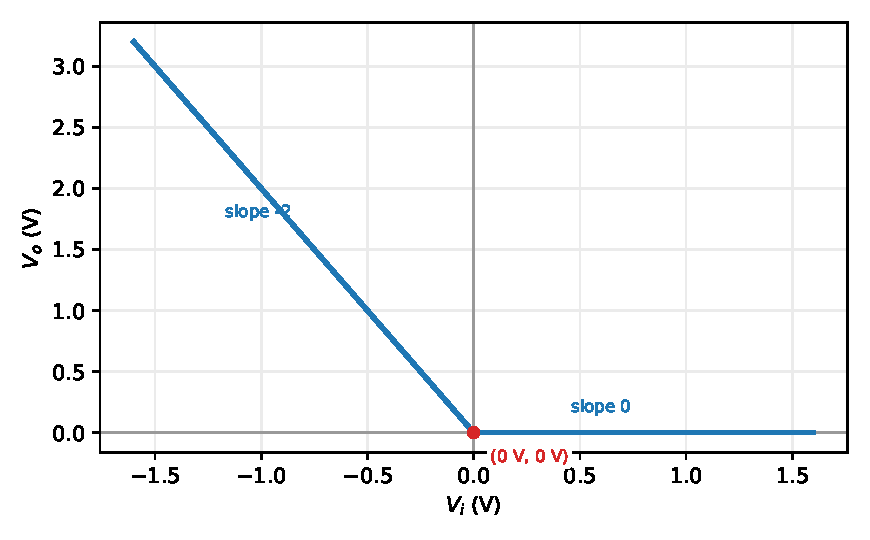
\includegraphics[width=0.62\linewidth,height=6cm,keepaspectratio]{p04_transfer}\end{center}
For $V_i(t) = 1\sin(2\pi\cdot 1000\,t)$ simply pass every instant of $V_i(t)$ through the characteristic above (each piece is a straight line, so each part of the sinusoid is scaled and shifted):\begin{center}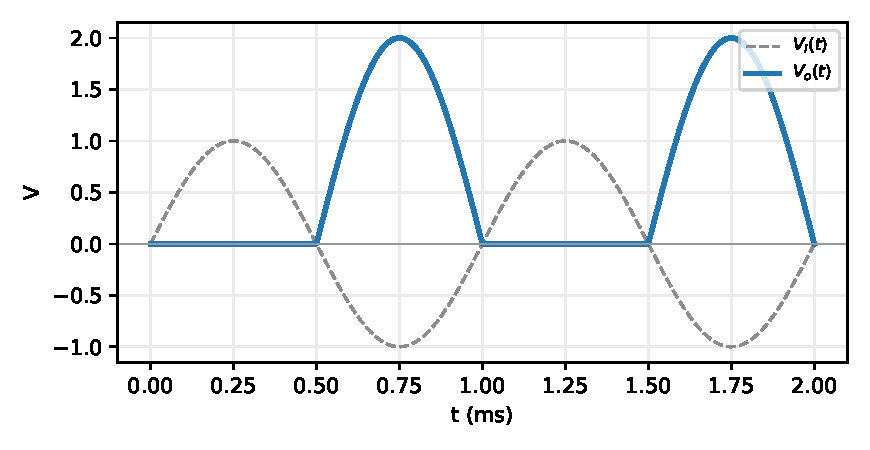
\includegraphics[width=0.62\linewidth,height=5cm,keepaspectratio]{p04_time}\end{center}

\begin{ansbox}
$V_o = \begin{cases} -2V_i & V_i < 0 \\ 0 & V_i > 0 \end{cases}$
\end{ansbox}

\newpage
\subsection*{Solution 3B.5 \hfill Easy}
\begin{center}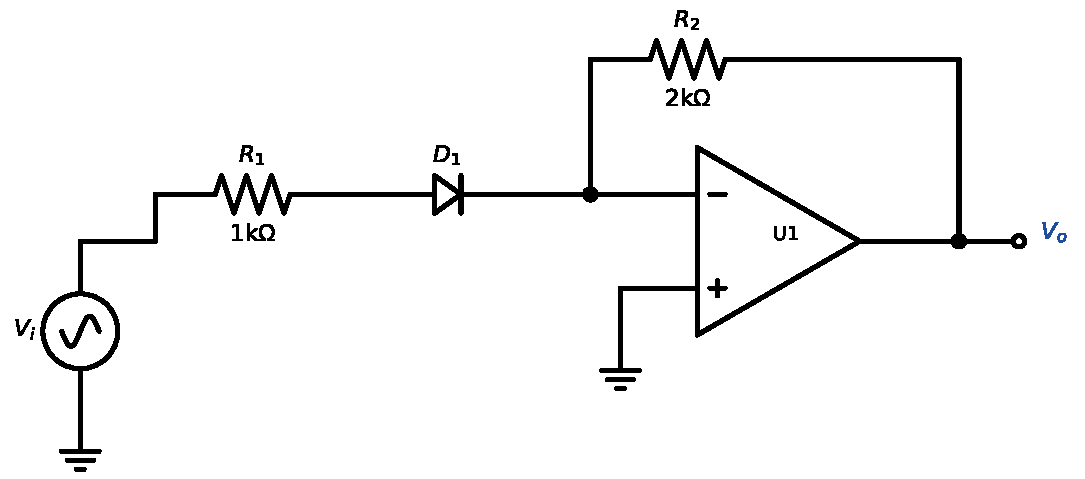
\includegraphics[width=0.9\linewidth,height=5cm,keepaspectratio]{p05_circuit}\end{center}
\solstep{1}{Model and method}Use the constant-voltage-drop model (tool T1): an OFF diode is an open circuit and needs $V_D<0.7$\,V; an ON diode is a $0.7$\,V source and needs $I_D>0$. With 1 diode there are $2$ ON/OFF combinations. For each one the circuit is linear: solve it with $V_i$ kept as a symbol, then check its assumptions --- each check is a condition on $V_i$ (tool T2). Op-amps are ideal ($A\to\infty$). Whether an op-amp has negative feedback can depend on the diode states, so decide it separately for every combination. Node names used below: $V_{-}$ = the op-amp's $-$ input; $V_{a}$ = node joining $D_{1}, R_{1}$.
\solstep{2}{Assume $D_{1}$ OFF}Replace $D_{1}$ OFF: an open circuit. U1 has negative feedback, so $V_- = V_+$ (virtual short) and no current flows into its inputs.

Equations (KCL at every node that is not an op-amp output, plus the diode voltages):\begin{align*}
&\text{KCL at }V_{-}\,(=0): && \frac{0 - V_{o}}{R_{2}} = 0 \\
&\text{KCL at }V_{a}: && \frac{V_{a} - V_i}{R_{1}} = 0
\end{align*}


Solving these linear equations (substitute one into the other, as in Lecture 2) gives, with $V_i$ kept as a symbol:\begin{align*}
V_{o} &= 0 \\
V_{D_{1}} = V_{a} - V_{-} &= V_i
\end{align*}


Check the assumptions: $V_{D_{1}} < 0.7$ $\Rightarrow$ $V_i < 0.7$\,V. So this state holds for $\boxed{V_i < 0.7}$, where $V_o = 0$.
\solstep{3}{Assume $D_{1}$ ON}Replace $D_{1}$ ON: a $0.7$\,V source ($V_{a} - V_{-} = 0.7$) carrying an unknown current $I_{D_{1}}$ from anode to cathode. U1 has negative feedback, so $V_- = V_+$ (virtual short) and no current flows into its inputs.

Equations (KCL at every node that is not an op-amp output, plus the diode voltages):\begin{align*}
&\text{KCL at }V_{-}\,(=0): && \frac{0 - V_{o}}{R_{2}} - I_{D_{1}} = 0 \\
&\text{KCL at }V_{a}: && \frac{V_{a} - V_i}{R_{1}} + I_{D_{1}} = 0 \\
&\text{D1 ON}: && V_{a} - 0 = 0.7
\end{align*}


Solving these linear equations (substitute one into the other, as in Lecture 2) gives, with $V_i$ kept as a symbol:\begin{align*}
V_{o} &= -2V_i + 1.4 \\
I_{D_{1}} &= V_i - 0.7\ \mathrm{mA}
\end{align*}


Check the assumptions: $I_{D_{1}} > 0$ $\Rightarrow$ $V_i > 0.7$\,V. So this state holds for $\boxed{V_i > 0.7}$, where $V_o = -2V_i + 1.4$.
\solstep{4}{Assemble and sketch}Put the valid states together:\[
V_o = \begin{cases} 0 & V_i < 0.7 \\ -2V_i + 1.4 & V_i > 0.7 \end{cases}
\]
Check: the pieces must meet at each breakpoint --- at $V_i=0.7$\,V both pieces give $V_o=0$\,V. \checkmark\begin{center}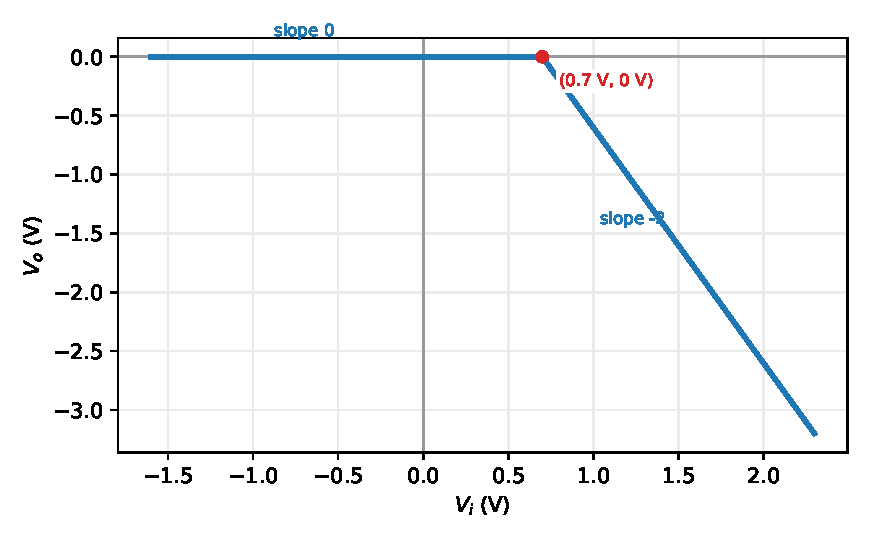
\includegraphics[width=0.62\linewidth,height=6cm,keepaspectratio]{p05_transfer}\end{center}
For $V_i(t) = 3\sin(2\pi\cdot 1000\,t)$ simply pass every instant of $V_i(t)$ through the characteristic above (each piece is a straight line, so each part of the sinusoid is scaled and shifted):\begin{center}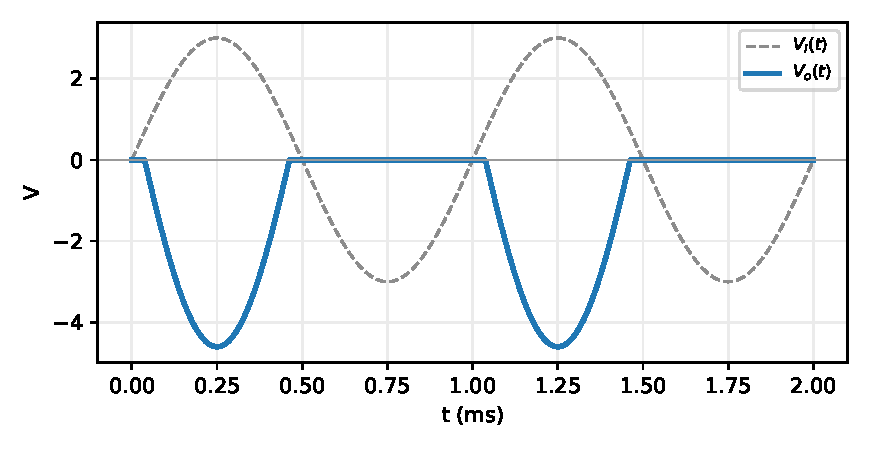
\includegraphics[width=0.62\linewidth,height=5cm,keepaspectratio]{p05_time}\end{center}

\begin{ansbox}
$V_o = \begin{cases} 0 & V_i < 0.7 \\ -2V_i + 1.4 & V_i > 0.7 \end{cases}$
\end{ansbox}

\newpage
\subsection*{Solution 3B.6 \hfill Easy}
\begin{center}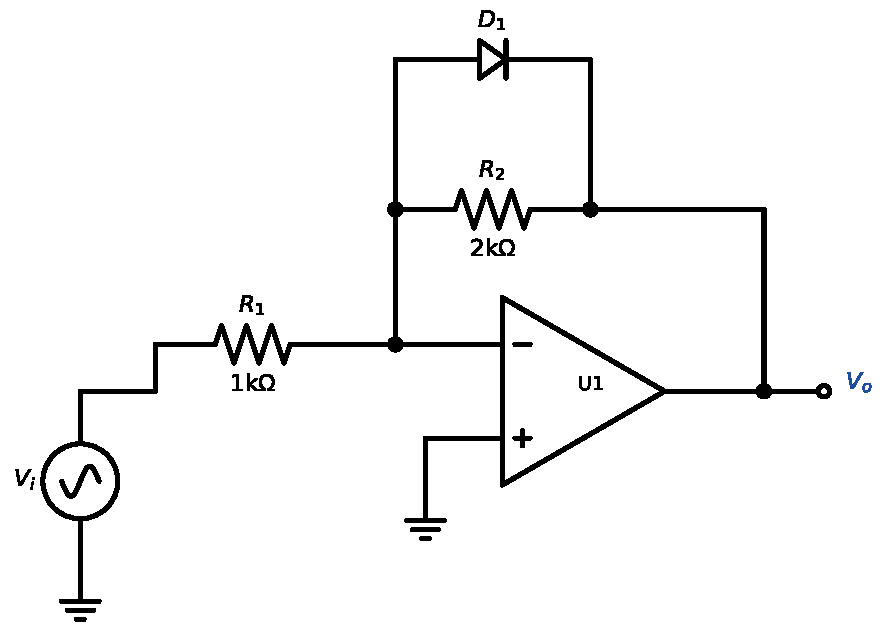
\includegraphics[width=0.9\linewidth,height=5cm,keepaspectratio]{p06_circuit}\end{center}
\solstep{1}{Model and method}Use the ideal-diode model (tool T1): an OFF diode is an open circuit and needs $V_D<0$; an ON diode is a short ($V_D=0$) and needs $I_D>0$. With 1 diode there are $2$ ON/OFF combinations. For each one the circuit is linear: solve it with $V_i$ kept as a symbol, then check its assumptions --- each check is a condition on $V_i$ (tool T2). Op-amps are ideal ($A\to\infty$). Whether an op-amp has negative feedback can depend on the diode states, so decide it separately for every combination. Node names used below: $V_{-}$ = the op-amp's $-$ input.
\solstep{2}{Assume $D_{1}$ OFF}Replace $D_{1}$ OFF: an open circuit. U1 has negative feedback, so $V_- = V_+$ (virtual short) and no current flows into its inputs.

Equations (KCL at every node that is not an op-amp output, plus the diode voltages):\begin{align*}
&\text{KCL at }V_{-}\,(=0): && \frac{0 - V_i}{R_{1}} + \frac{0 - V_{o}}{R_{2}} = 0
\end{align*}


Solving these linear equations (substitute one into the other, as in Lecture 2) gives, with $V_i$ kept as a symbol:\begin{align*}
V_{o} &= -2V_i \\
V_{D_{1}} = V_{-} - V_{o} &= 2V_i
\end{align*}


Check the assumptions: $V_{D_{1}} < 0$ $\Rightarrow$ $V_i < 0$\,V. So this state holds for $\boxed{V_i < 0}$, where $V_o = -2V_i$.
\solstep{3}{Assume $D_{1}$ ON}Replace $D_{1}$ ON: a $0$\,V source ($V_{-} - V_{o} = 0$) carrying an unknown current $I_{D_{1}}$ from anode to cathode. U1 has negative feedback, so $V_- = V_+$ (virtual short) and no current flows into its inputs.

Equations (KCL at every node that is not an op-amp output, plus the diode voltages):\begin{align*}
&\text{KCL at }V_{-}\,(=0): && \frac{0 - V_i}{R_{1}} + \frac{0 - V_{o}}{R_{2}} + I_{D_{1}} = 0 \\
&\text{D1 ON}: && 0 - V_{o} = 0
\end{align*}


Solving these linear equations (substitute one into the other, as in Lecture 2) gives, with $V_i$ kept as a symbol:\begin{align*}
V_{o} &= 0 \\
I_{D_{1}} &= V_i\ \mathrm{mA}
\end{align*}


Check the assumptions: $I_{D_{1}} > 0$ $\Rightarrow$ $V_i > 0$\,V. So this state holds for $\boxed{V_i > 0}$, where $V_o = 0$.
\solstep{4}{Assemble and sketch}Put the valid states together:\[
V_o = \begin{cases} -2V_i & V_i < 0 \\ 0 & V_i > 0 \end{cases}
\]
Check: the pieces must meet at each breakpoint --- at $V_i=0$\,V both pieces give $V_o=0$\,V. \checkmark\begin{center}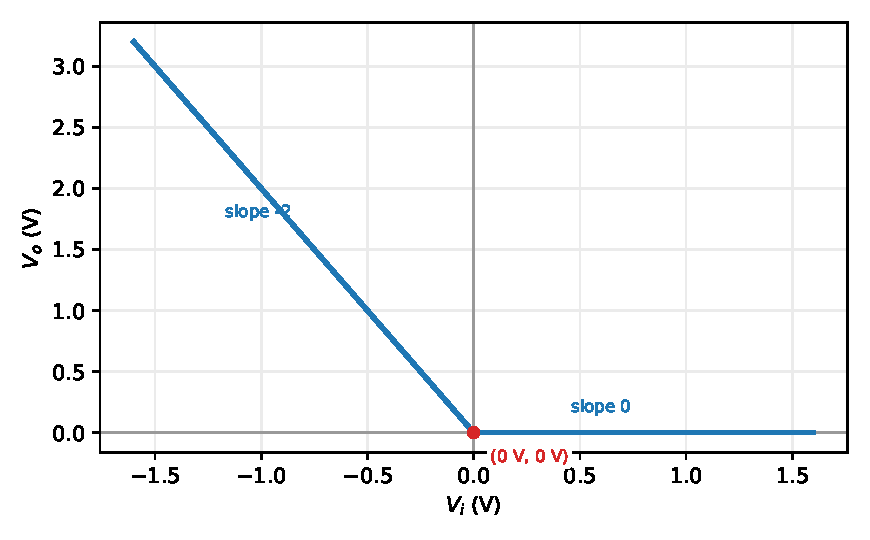
\includegraphics[width=0.62\linewidth,height=6cm,keepaspectratio]{p06_transfer}\end{center}
For $V_i(t) = 2\sin(2\pi\cdot 1000\,t)$ simply pass every instant of $V_i(t)$ through the characteristic above (each piece is a straight line, so each part of the sinusoid is scaled and shifted):\begin{center}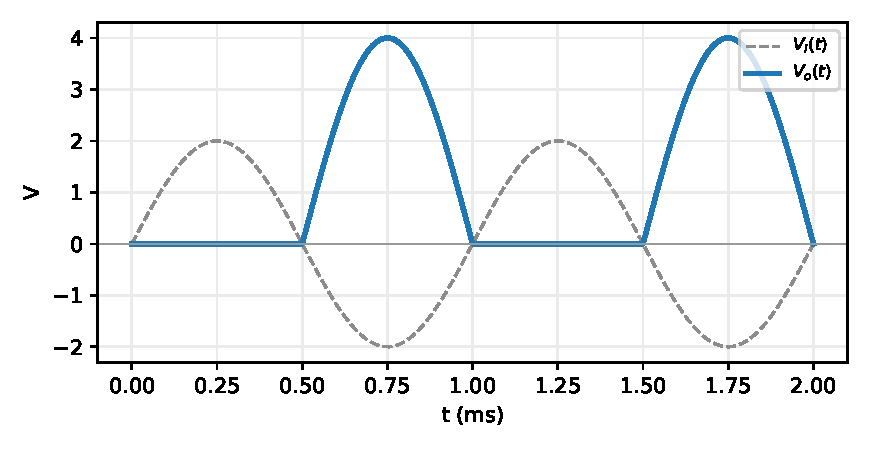
\includegraphics[width=0.62\linewidth,height=5cm,keepaspectratio]{p06_time}\end{center}

\begin{ansbox}
$V_o = \begin{cases} -2V_i & V_i < 0 \\ 0 & V_i > 0 \end{cases}$
\end{ansbox}

\newpage
\subsection*{Solution 3B.7 \hfill Medium}
\begin{center}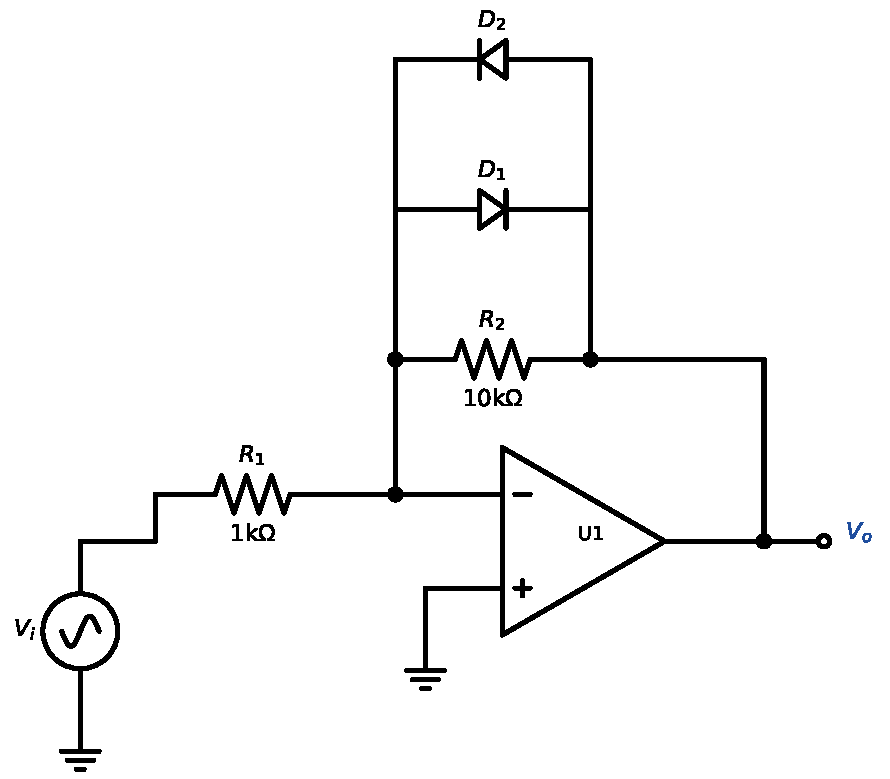
\includegraphics[width=0.9\linewidth,height=5cm,keepaspectratio]{p07_circuit}\end{center}
\solstep{1}{Model and method}Use the constant-voltage-drop model (tool T1): an OFF diode is an open circuit and needs $V_D<0.7$\,V; an ON diode is a $0.7$\,V source and needs $I_D>0$. With 2 diodes there are $4$ ON/OFF combinations. For each one the circuit is linear: solve it with $V_i$ kept as a symbol, then check its assumptions --- each check is a condition on $V_i$ (tool T2). Op-amps are ideal ($A\to\infty$). Whether an op-amp has negative feedback can depend on the diode states, so decide it separately for every combination. Node names used below: $V_{-}$ = the op-amp's $-$ input.
\solstep{2}{Assume $D_{1}$ OFF, $D_{2}$ ON}Replace $D_{1}$ OFF: an open circuit; $D_{2}$ ON: a $0.7$\,V source ($V_{o} - V_{-} = 0.7$) carrying an unknown current $I_{D_{2}}$ from anode to cathode. U1 has negative feedback, so $V_- = V_+$ (virtual short) and no current flows into its inputs.

Equations (KCL at every node that is not an op-amp output, plus the diode voltages):\begin{align*}
&\text{KCL at }V_{-}\,(=0): && \frac{0 - V_i}{R_{1}} + \frac{0 - V_{o}}{R_{2}} - I_{D_{2}} = 0 \\
&\text{D2 ON}: && V_{o} - 0 = 0.7
\end{align*}


Solving these linear equations (substitute one into the other, as in Lecture 2) gives, with $V_i$ kept as a symbol:\begin{align*}
V_{o} &= 0.7 \\
V_{D_{1}} = V_{-} - V_{o} &= -0.7 \\
I_{D_{2}} &= -V_i - 0.07\ \mathrm{mA}
\end{align*}


Check the assumptions: $V_{D_{1}} < 0.7$ $\Rightarrow$ true for every $V_i$; $I_{D_{2}} > 0$ $\Rightarrow$ $V_i < -0.07$\,V. So this state holds for $\boxed{V_i < -0.07}$, where $V_o = 0.7$.
\solstep{3}{Assume $D_{1}$ OFF, $D_{2}$ OFF}Replace $D_{1}$ OFF: an open circuit; $D_{2}$ OFF: an open circuit. U1 has negative feedback, so $V_- = V_+$ (virtual short) and no current flows into its inputs.

Equations (KCL at every node that is not an op-amp output, plus the diode voltages):\begin{align*}
&\text{KCL at }V_{-}\,(=0): && \frac{0 - V_i}{R_{1}} + \frac{0 - V_{o}}{R_{2}} = 0
\end{align*}


Solving these linear equations (substitute one into the other, as in Lecture 2) gives, with $V_i$ kept as a symbol:\begin{align*}
V_{o} &= -10V_i \\
V_{D_{1}} = V_{-} - V_{o} &= 10V_i \\
V_{D_{2}} = V_{o} - V_{-} &= -10V_i
\end{align*}


Check the assumptions: $V_{D_{1}} < 0.7$ $\Rightarrow$ $V_i < 0.07$\,V; $V_{D_{2}} < 0.7$ $\Rightarrow$ $V_i > -0.07$\,V. So this state holds for $\boxed{-0.07 < V_i < 0.07}$, where $V_o = -10V_i$.
\solstep{4}{Assume $D_{1}$ ON, $D_{2}$ OFF}Replace $D_{1}$ ON: a $0.7$\,V source ($V_{-} - V_{o} = 0.7$) carrying an unknown current $I_{D_{1}}$ from anode to cathode; $D_{2}$ OFF: an open circuit. U1 has negative feedback, so $V_- = V_+$ (virtual short) and no current flows into its inputs.

Equations (KCL at every node that is not an op-amp output, plus the diode voltages):\begin{align*}
&\text{KCL at }V_{-}\,(=0): && \frac{0 - V_i}{R_{1}} + \frac{0 - V_{o}}{R_{2}} + I_{D_{1}} = 0 \\
&\text{D1 ON}: && 0 - V_{o} = 0.7
\end{align*}


Solving these linear equations (substitute one into the other, as in Lecture 2) gives, with $V_i$ kept as a symbol:\begin{align*}
V_{o} &= -0.7 \\
I_{D_{1}} &= V_i - 0.07\ \mathrm{mA} \\
V_{D_{2}} = V_{o} - V_{-} &= -0.7
\end{align*}


Check the assumptions: $I_{D_{1}} > 0$ $\Rightarrow$ $V_i > 0.07$\,V; $V_{D_{2}} < 0.7$ $\Rightarrow$ true for every $V_i$. So this state holds for $\boxed{V_i > 0.07}$, where $V_o = -0.7$.
\solstep{5}{The other combinations}\begin{itemize}[leftmargin=*,itemsep=2pt]
\item $D_{1}$ ON, $D_{2}$ ON: the ON diodes would have to hold the same node at two different voltages at once, which no circuit can do --- these cannot all hold, so this state never occurs.
\end{itemize}

\solstep{6}{Assemble and sketch}Put the valid states together:\[
V_o = \begin{cases} 0.7 & V_i < -0.07 \\ -10V_i & -0.07 < V_i < 0.07 \\ -0.7 & V_i > 0.07 \end{cases}
\]
Check: the pieces must meet at each breakpoint --- at $V_i=-0.07$\,V both pieces give $V_o=0.7$\,V; at $V_i=0.07$\,V both pieces give $V_o=-0.7$\,V. \checkmark\begin{center}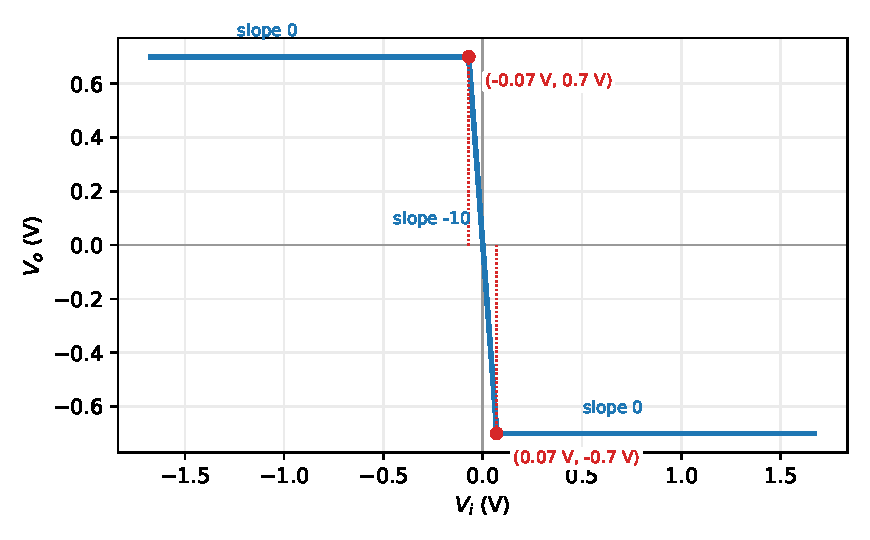
\includegraphics[width=0.62\linewidth,height=6cm,keepaspectratio]{p07_transfer}\end{center}
For $V_i(t) = 0.5\sin(2\pi\cdot 1000\,t)$ simply pass every instant of $V_i(t)$ through the characteristic above (each piece is a straight line, so each part of the sinusoid is scaled and shifted):\begin{center}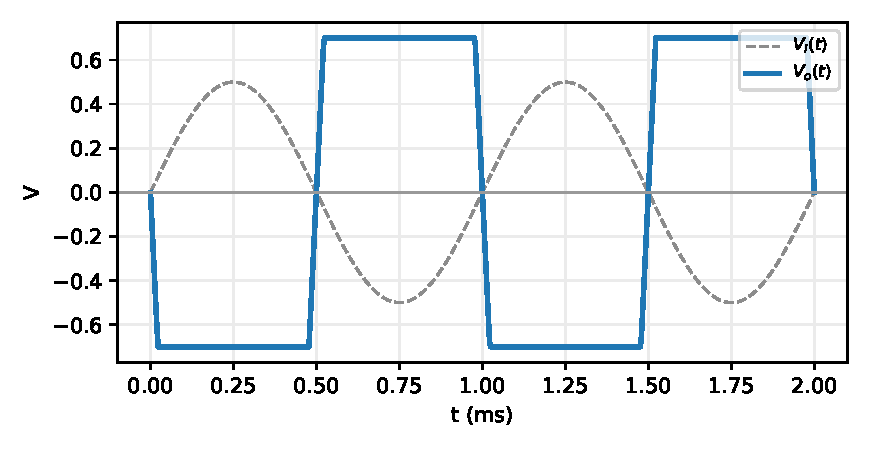
\includegraphics[width=0.62\linewidth,height=5cm,keepaspectratio]{p07_time}\end{center}

\begin{ansbox}
$V_o = \begin{cases} 0.7 & V_i < -0.07 \\ -10V_i & -0.07 < V_i < 0.07 \\ -0.7 & V_i > 0.07 \end{cases}$
\end{ansbox}

\newpage
\subsection*{Solution 3B.8 \hfill Medium}
\begin{center}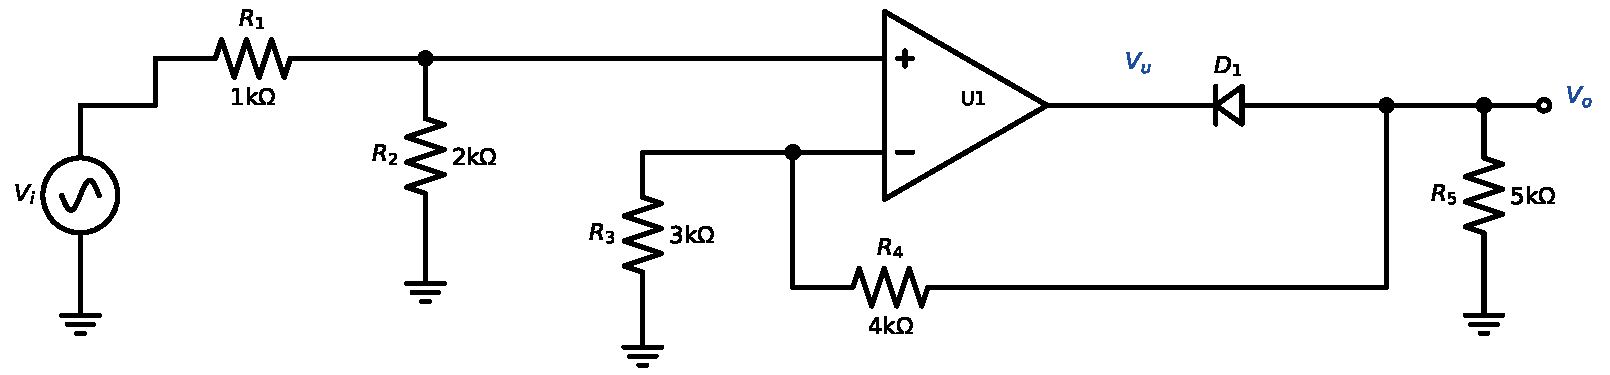
\includegraphics[width=0.9\linewidth,height=5cm,keepaspectratio]{p08_circuit}\end{center}
\solstep{1}{Model and method}Use the constant-voltage-drop model (tool T1): an OFF diode is an open circuit and needs $V_D<0.7$\,V; an ON diode is a $0.7$\,V source and needs $I_D>0$. With 1 diode there are $2$ ON/OFF combinations. For each one the circuit is linear: solve it with $V_i$ kept as a symbol, then check its assumptions --- each check is a condition on $V_i$ (tool T2). Op-amps are ideal ($A\to\infty$). Whether an op-amp has negative feedback can depend on the diode states, so decide it separately for every combination. Node names used below: $V_{+}$ = the op-amp's $+$ input; $V_{-}$ = the op-amp's $-$ input.
\solstep{2}{Assume $D_{1}$ ON}Replace $D_{1}$ ON: a $0.7$\,V source ($V_{o} - V_{u} = 0.7$) carrying an unknown current $I_{D_{1}}$ from anode to cathode. U1 has negative feedback, so $V_- = V_+$ (virtual short) and no current flows into its inputs.

Equations (KCL at every node that is not an op-amp output, plus the diode voltages):\begin{align*}
&\text{KCL at }V_{+}: && \frac{V_{+} - V_i}{R_{1}} + \frac{V_{+}}{R_{2}} = 0 \\
&\text{KCL at }V_{-}\,(=V_{+}): && \frac{V_{+}}{R_{3}} + \frac{V_{+} - V_{o}}{R_{4}} = 0 \\
&\text{KCL at }V_{o}: && \frac{V_{o} - V_{+}}{R_{4}} + \frac{V_{o}}{R_{5}} + I_{D_{1}} = 0 \\
&\text{D1 ON}: && V_{o} - V_{u} = 0.7
\end{align*}


Solving these linear equations (substitute one into the other, as in Lecture 2) gives, with $V_i$ kept as a symbol:\begin{align*}
V_{o} &= 1.556V_i \\
I_{D_{1}} &= -0.5333V_i\ \mathrm{mA}
\end{align*}


Check the assumptions: $I_{D_{1}} > 0$ $\Rightarrow$ $V_i < 0$\,V. So this state holds for $\boxed{V_i < 0}$, where $V_o = 1.556V_i$.
\solstep{3}{Assume $D_{1}$ OFF}Replace $D_{1}$ OFF: an open circuit. With this assumption U1 has no feedback path from its output back to its $-$ input: it runs \emph{open-loop}, $V_{u} = A(V_+ - V_-)$ with $A\to\infty$, so its output is pushed to $\pm\infty$ (in practice, a supply rail) unless $V_+ = V_-$ exactly.

Equations (KCL at every node that is not an op-amp output, plus the diode voltages):\begin{align*}
&\text{KCL at }V_{+}: && \frac{V_{+} - V_i}{R_{1}} + \frac{V_{+}}{R_{2}} = 0 \\
&\text{KCL at }V_{-}: && \frac{V_{-}}{R_{3}} + \frac{V_{-} - V_{o}}{R_{4}} = 0 \\
&\text{KCL at }V_{o}: && \frac{V_{o} - V_{-}}{R_{4}} + \frac{V_{o}}{R_{5}} = 0
\end{align*}


Solving these linear equations (substitute one into the other, as in Lecture 2) gives, with $V_i$ kept as a symbol:\begin{align*}
V_{o} &= 0 \\
V_{D_{1}} = V_{o} - V_{u} &\approx A\left(-0.6667V_i\right)
\end{align*}


Check the assumptions: $V_{D_{1}} < 0.7$; since $A\to\infty$ this needs $-0.6667V_i < 0$ $\Rightarrow$ $V_i > 0$\,V. So this state holds for $\boxed{V_i > 0}$, where $V_o = 0$.
\solstep{4}{Assemble and sketch}Put the valid states together:\[
V_o = \begin{cases} 1.556V_i & V_i < 0 \\ 0 & V_i > 0 \end{cases}
\]
Check: the pieces must meet at each breakpoint --- at $V_i=0$\,V both pieces give $V_o=0$\,V. \checkmark\begin{center}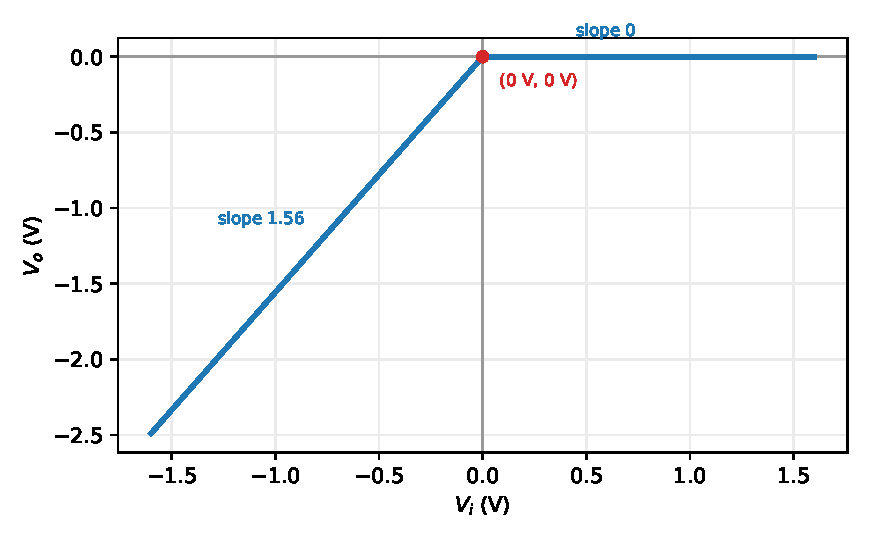
\includegraphics[width=0.62\linewidth,height=6cm,keepaspectratio]{p08_transfer}\end{center}
For $V_i(t) = 2\sin(2\pi\cdot 500\,t)$ simply pass every instant of $V_i(t)$ through the characteristic above (each piece is a straight line, so each part of the sinusoid is scaled and shifted):\begin{center}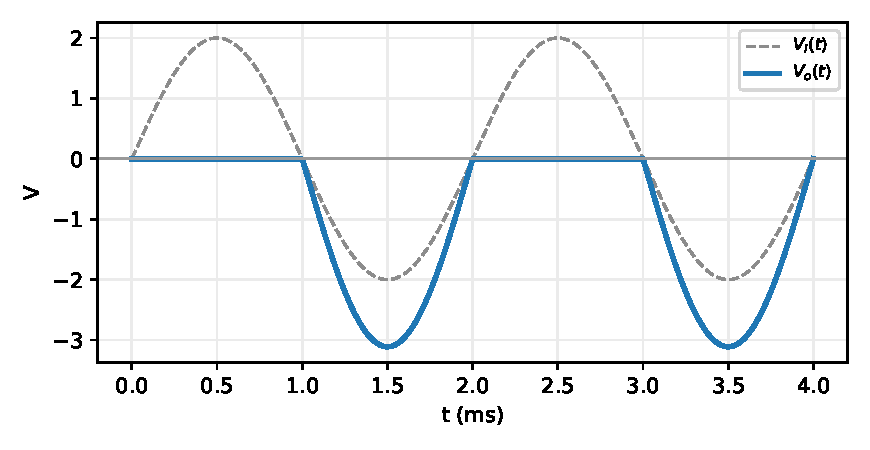
\includegraphics[width=0.62\linewidth,height=5cm,keepaspectratio]{p08_time}\end{center}

\begin{ansbox}
$V_o = \begin{cases} 1.556V_i & V_i < 0 \\ 0 & V_i > 0 \end{cases}$
\end{ansbox}

\newpage
\subsection*{Solution 3B.9 \hfill Medium}
\begin{center}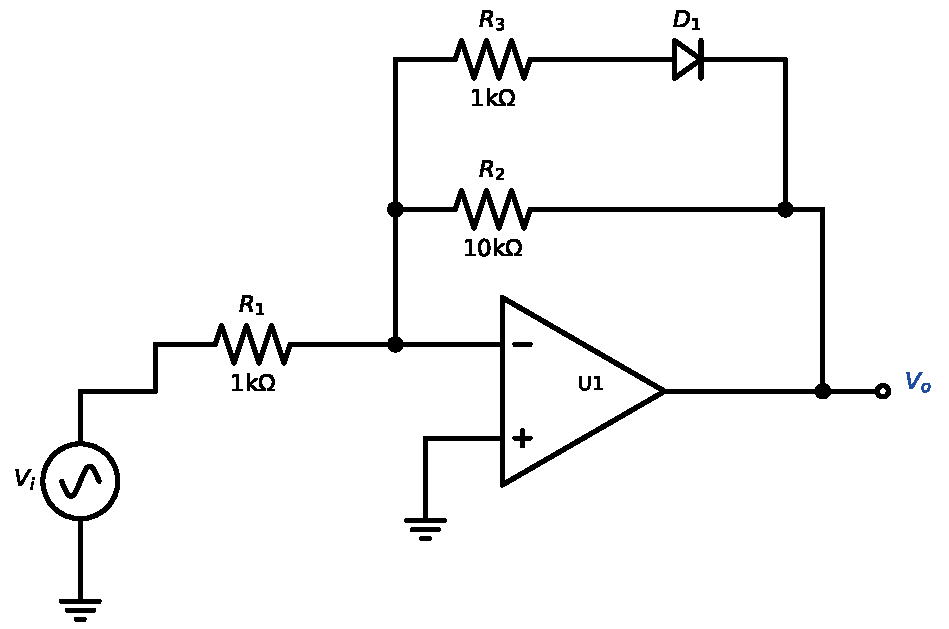
\includegraphics[width=0.9\linewidth,height=5cm,keepaspectratio]{p09_circuit}\end{center}
\solstep{1}{Model and method}Use the constant-voltage-drop model (tool T1): an OFF diode is an open circuit and needs $V_D<0.7$\,V; an ON diode is a $0.7$\,V source and needs $I_D>0$. With 1 diode there are $2$ ON/OFF combinations. For each one the circuit is linear: solve it with $V_i$ kept as a symbol, then check its assumptions --- each check is a condition on $V_i$ (tool T2). Op-amps are ideal ($A\to\infty$). Whether an op-amp has negative feedback can depend on the diode states, so decide it separately for every combination. Node names used below: $V_{-}$ = the op-amp's $-$ input; $V_{a}$ = node joining $D_{1}, R_{3}$.
\solstep{2}{Assume $D_{1}$ OFF}Replace $D_{1}$ OFF: an open circuit. U1 has negative feedback, so $V_- = V_+$ (virtual short) and no current flows into its inputs.

Equations (KCL at every node that is not an op-amp output, plus the diode voltages):\begin{align*}
&\text{KCL at }V_{-}\,(=0): && \frac{0 - V_i}{R_{1}} + \frac{0 - V_{o}}{R_{2}} + \frac{0 - V_{a}}{R_{3}} = 0 \\
&\text{KCL at }V_{a}: && \frac{V_{a}}{R_{3}} = 0
\end{align*}


Solving these linear equations (substitute one into the other, as in Lecture 2) gives, with $V_i$ kept as a symbol:\begin{align*}
V_{o} &= -10V_i \\
V_{D_{1}} = V_{a} - V_{o} &= 10V_i
\end{align*}


Check the assumptions: $V_{D_{1}} < 0.7$ $\Rightarrow$ $V_i < 0.07$\,V. So this state holds for $\boxed{V_i < 0.07}$, where $V_o = -10V_i$.
\solstep{3}{Assume $D_{1}$ ON}Replace $D_{1}$ ON: a $0.7$\,V source ($V_{a} - V_{o} = 0.7$) carrying an unknown current $I_{D_{1}}$ from anode to cathode. U1 has negative feedback, so $V_- = V_+$ (virtual short) and no current flows into its inputs.

Equations (KCL at every node that is not an op-amp output, plus the diode voltages):\begin{align*}
&\text{KCL at }V_{-}\,(=0): && \frac{0 - V_i}{R_{1}} + \frac{0 - V_{o}}{R_{2}} + \frac{0 - V_{a}}{R_{3}} = 0 \\
&\text{KCL at }V_{a}: && \frac{V_{a}}{R_{3}} + I_{D_{1}} = 0 \\
&\text{D1 ON}: && V_{a} - V_{o} = 0.7
\end{align*}


Solving these linear equations (substitute one into the other, as in Lecture 2) gives, with $V_i$ kept as a symbol:\begin{align*}
V_{o} &= -0.9091V_i - 0.6364 \\
I_{D_{1}} &= 0.9091V_i - 0.06364\ \mathrm{mA}
\end{align*}


Check the assumptions: $I_{D_{1}} > 0$ $\Rightarrow$ $V_i > 0.07$\,V. So this state holds for $\boxed{V_i > 0.07}$, where $V_o = -0.9091V_i - 0.6364$.
\solstep{4}{Assemble and sketch}Put the valid states together:\[
V_o = \begin{cases} -10V_i & V_i < 0.07 \\ -0.9091V_i - 0.6364 & V_i > 0.07 \end{cases}
\]
Check: the pieces must meet at each breakpoint --- at $V_i=0.07$\,V both pieces give $V_o=-0.7$\,V. \checkmark\begin{center}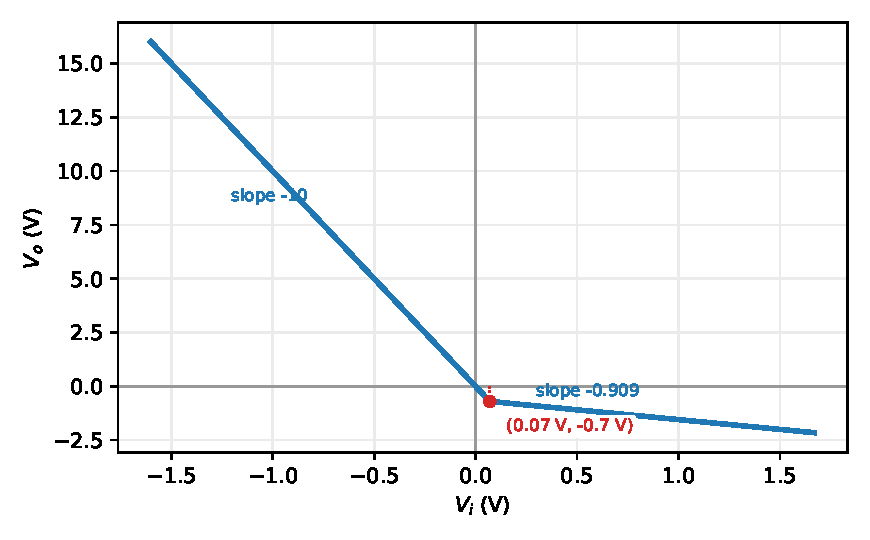
\includegraphics[width=0.62\linewidth,height=6cm,keepaspectratio]{p09_transfer}\end{center}
For $V_i(t) = 1\sin(2\pi\cdot 1000\,t)$ simply pass every instant of $V_i(t)$ through the characteristic above (each piece is a straight line, so each part of the sinusoid is scaled and shifted):\begin{center}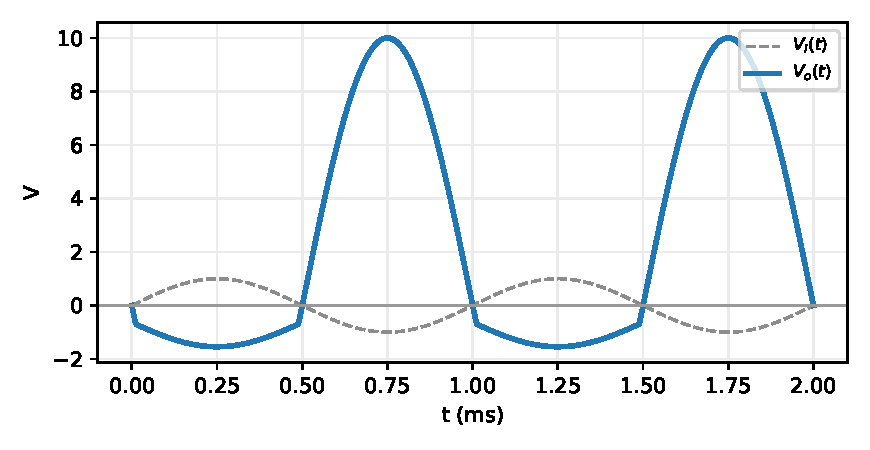
\includegraphics[width=0.62\linewidth,height=5cm,keepaspectratio]{p09_time}\end{center}

\begin{ansbox}
$V_o = \begin{cases} -10V_i & V_i < 0.07 \\ -0.9091V_i - 0.6364 & V_i > 0.07 \end{cases}$
\end{ansbox}

\newpage
\subsection*{Solution 3B.10 \hfill Medium}
\begin{center}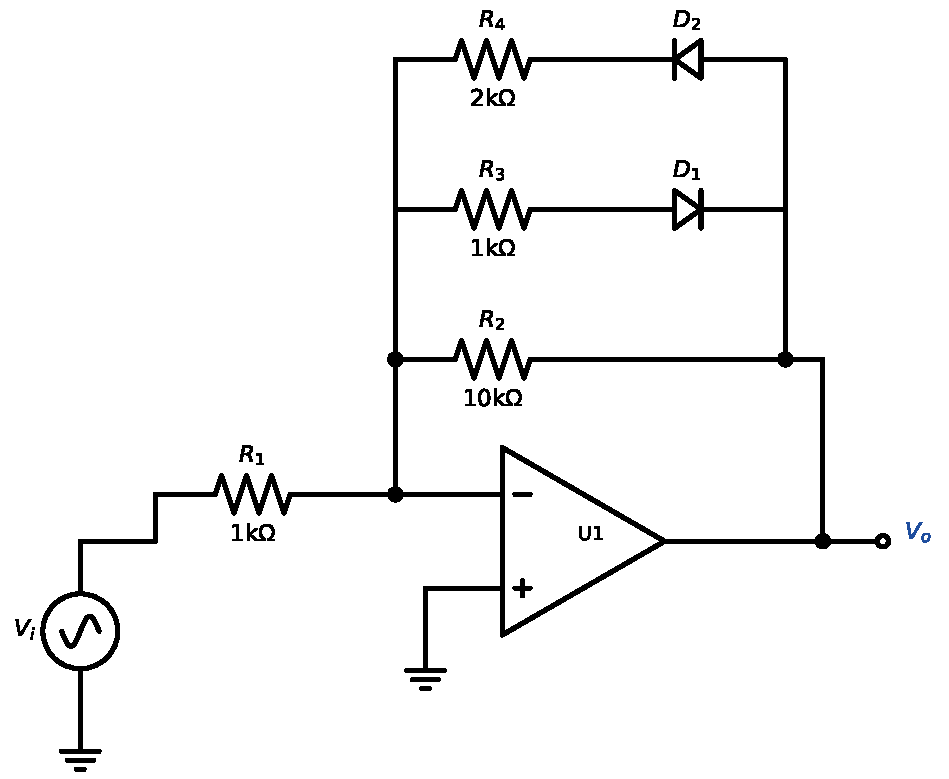
\includegraphics[width=0.9\linewidth,height=5cm,keepaspectratio]{p10_circuit}\end{center}
\solstep{1}{Model and method}Use the constant-voltage-drop model (tool T1): an OFF diode is an open circuit and needs $V_D<0.7$\,V; an ON diode is a $0.7$\,V source and needs $I_D>0$. With 2 diodes there are $4$ ON/OFF combinations. For each one the circuit is linear: solve it with $V_i$ kept as a symbol, then check its assumptions --- each check is a condition on $V_i$ (tool T2). Op-amps are ideal ($A\to\infty$). Whether an op-amp has negative feedback can depend on the diode states, so decide it separately for every combination. Node names used below: $V_{-}$ = the op-amp's $-$ input; $V_{a}$ = node joining $D_{1}, R_{3}$; $V_{b}$ = node joining $D_{2}, R_{4}$.
\solstep{2}{Assume $D_{1}$ OFF, $D_{2}$ ON}Replace $D_{1}$ OFF: an open circuit; $D_{2}$ ON: a $0.7$\,V source ($V_{o} - V_{b} = 0.7$) carrying an unknown current $I_{D_{2}}$ from anode to cathode. U1 has negative feedback, so $V_- = V_+$ (virtual short) and no current flows into its inputs.

Equations (KCL at every node that is not an op-amp output, plus the diode voltages):\begin{align*}
&\text{KCL at }V_{-}\,(=0): && \frac{0 - V_i}{R_{1}} + \frac{0 - V_{o}}{R_{2}} + \frac{0 - V_{a}}{R_{3}} + \frac{0 - V_{b}}{R_{4}} = 0 \\
&\text{KCL at }V_{a}: && \frac{V_{a}}{R_{3}} = 0 \\
&\text{KCL at }V_{b}: && \frac{V_{b}}{R_{4}} - I_{D_{2}} = 0 \\
&\text{D2 ON}: && V_{o} - V_{b} = 0.7
\end{align*}


Solving these linear equations (substitute one into the other, as in Lecture 2) gives, with $V_i$ kept as a symbol:\begin{align*}
V_{o} &= -1.667V_i + 0.5833 \\
V_{D_{1}} = V_{a} - V_{o} &= 1.667V_i - 0.5833 \\
I_{D_{2}} &= -0.8333V_i - 0.05833\ \mathrm{mA}
\end{align*}


Check the assumptions: $V_{D_{1}} < 0.7$ $\Rightarrow$ $V_i < 0.77$\,V; $I_{D_{2}} > 0$ $\Rightarrow$ $V_i < -0.07$\,V. So this state holds for $\boxed{V_i < -0.07}$, where $V_o = -1.667V_i + 0.5833$.
\solstep{3}{Assume $D_{1}$ OFF, $D_{2}$ OFF}Replace $D_{1}$ OFF: an open circuit; $D_{2}$ OFF: an open circuit. U1 has negative feedback, so $V_- = V_+$ (virtual short) and no current flows into its inputs.

Equations (KCL at every node that is not an op-amp output, plus the diode voltages):\begin{align*}
&\text{KCL at }V_{-}\,(=0): && \frac{0 - V_i}{R_{1}} + \frac{0 - V_{o}}{R_{2}} + \frac{0 - V_{a}}{R_{3}} + \frac{0 - V_{b}}{R_{4}} = 0 \\
&\text{KCL at }V_{a}: && \frac{V_{a}}{R_{3}} = 0 \\
&\text{KCL at }V_{b}: && \frac{V_{b}}{R_{4}} = 0
\end{align*}


Solving these linear equations (substitute one into the other, as in Lecture 2) gives, with $V_i$ kept as a symbol:\begin{align*}
V_{o} &= -10V_i \\
V_{D_{1}} = V_{a} - V_{o} &= 10V_i \\
V_{D_{2}} = V_{o} - V_{b} &= -10V_i
\end{align*}


Check the assumptions: $V_{D_{1}} < 0.7$ $\Rightarrow$ $V_i < 0.07$\,V; $V_{D_{2}} < 0.7$ $\Rightarrow$ $V_i > -0.07$\,V. So this state holds for $\boxed{-0.07 < V_i < 0.07}$, where $V_o = -10V_i$.
\solstep{4}{Assume $D_{1}$ ON, $D_{2}$ OFF}Replace $D_{1}$ ON: a $0.7$\,V source ($V_{a} - V_{o} = 0.7$) carrying an unknown current $I_{D_{1}}$ from anode to cathode; $D_{2}$ OFF: an open circuit. U1 has negative feedback, so $V_- = V_+$ (virtual short) and no current flows into its inputs.

Equations (KCL at every node that is not an op-amp output, plus the diode voltages):\begin{align*}
&\text{KCL at }V_{-}\,(=0): && \frac{0 - V_i}{R_{1}} + \frac{0 - V_{o}}{R_{2}} + \frac{0 - V_{a}}{R_{3}} + \frac{0 - V_{b}}{R_{4}} = 0 \\
&\text{KCL at }V_{a}: && \frac{V_{a}}{R_{3}} + I_{D_{1}} = 0 \\
&\text{KCL at }V_{b}: && \frac{V_{b}}{R_{4}} = 0 \\
&\text{D1 ON}: && V_{a} - V_{o} = 0.7
\end{align*}


Solving these linear equations (substitute one into the other, as in Lecture 2) gives, with $V_i$ kept as a symbol:\begin{align*}
V_{o} &= -0.9091V_i - 0.6364 \\
I_{D_{1}} &= 0.9091V_i - 0.06364\ \mathrm{mA} \\
V_{D_{2}} = V_{o} - V_{b} &= -0.9091V_i - 0.6364
\end{align*}


Check the assumptions: $I_{D_{1}} > 0$ $\Rightarrow$ $V_i > 0.07$\,V; $V_{D_{2}} < 0.7$ $\Rightarrow$ $V_i > -1.47$\,V. So this state holds for $\boxed{V_i > 0.07}$, where $V_o = -0.9091V_i - 0.6364$.
\solstep{5}{The other combinations}\begin{itemize}[leftmargin=*,itemsep=2pt]
\item $D_{1}$ ON, $D_{2}$ ON: $I_{D_{1}}>0$ needs $V_i > 0.77$; $I_{D_{2}}>0$ needs $V_i < -1.47$ --- these cannot all hold, so this state never occurs.
\end{itemize}

\solstep{6}{Assemble and sketch}Put the valid states together:\[
V_o = \begin{cases} -1.667V_i + 0.5833 & V_i < -0.07 \\ -10V_i & -0.07 < V_i < 0.07 \\ -0.9091V_i - 0.6364 & V_i > 0.07 \end{cases}
\]
Check: the pieces must meet at each breakpoint --- at $V_i=-0.07$\,V both pieces give $V_o=0.7$\,V; at $V_i=0.07$\,V both pieces give $V_o=-0.7$\,V. \checkmark\begin{center}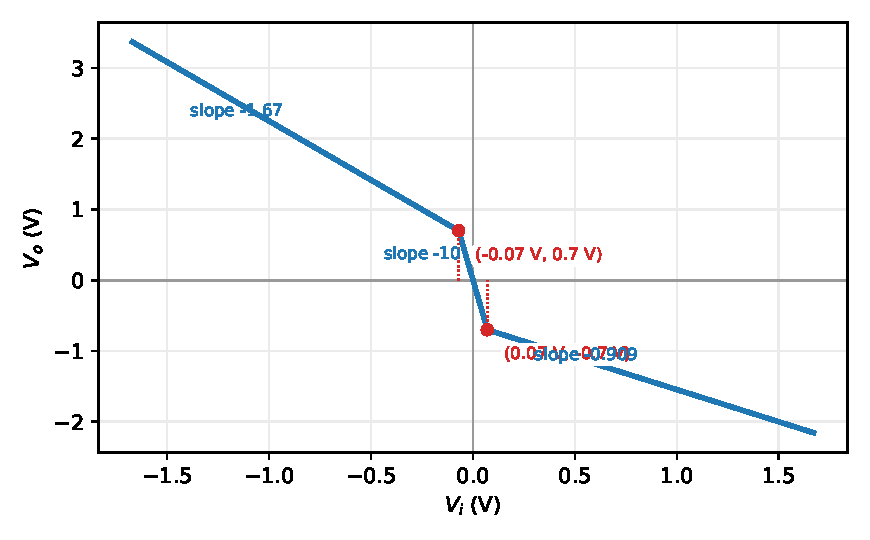
\includegraphics[width=0.62\linewidth,height=6cm,keepaspectratio]{p10_transfer}\end{center}
For $V_i(t) = 1\sin(2\pi\cdot 1000\,t)$ simply pass every instant of $V_i(t)$ through the characteristic above (each piece is a straight line, so each part of the sinusoid is scaled and shifted):\begin{center}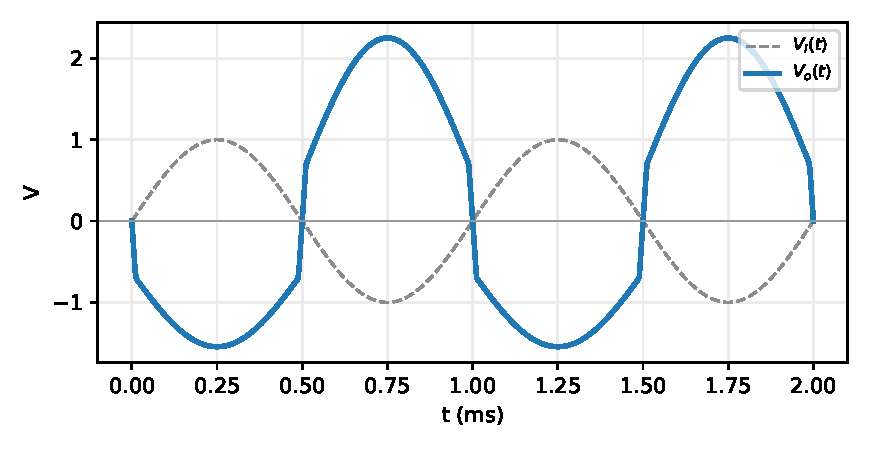
\includegraphics[width=0.62\linewidth,height=5cm,keepaspectratio]{p10_time}\end{center}

\begin{ansbox}
$V_o = \begin{cases} -1.667V_i + 0.5833 & V_i < -0.07 \\ -10V_i & -0.07 < V_i < 0.07 \\ -0.9091V_i - 0.6364 & V_i > 0.07 \end{cases}$
\end{ansbox}

\newpage
\subsection*{Solution 3B.11 \hfill Medium}
\begin{center}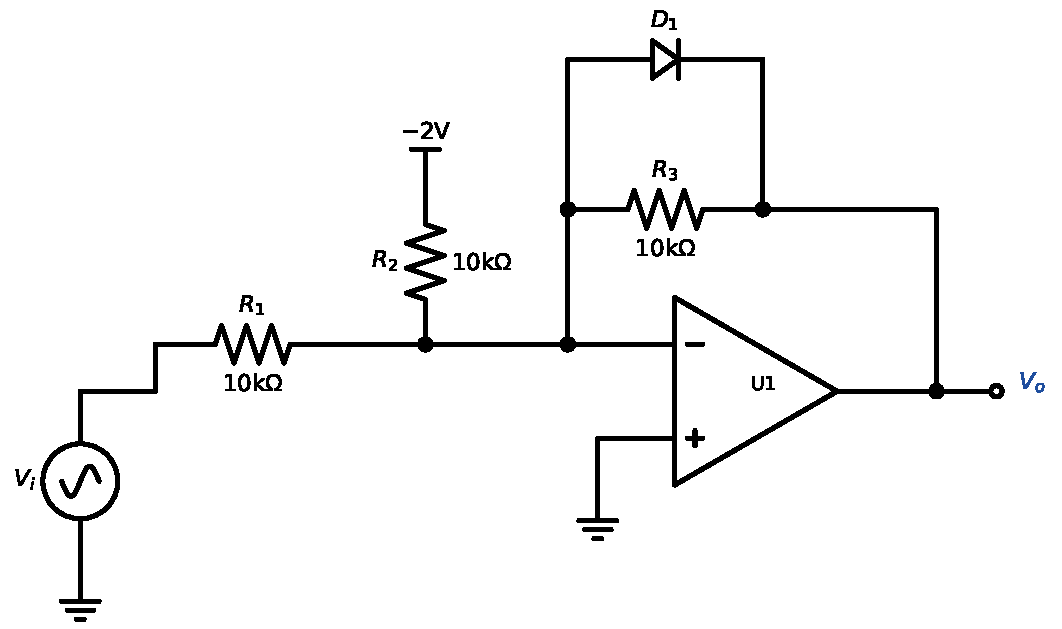
\includegraphics[width=0.9\linewidth,height=5cm,keepaspectratio]{p11_circuit}\end{center}
\solstep{1}{Model and method}Use the constant-voltage-drop model (tool T1): an OFF diode is an open circuit and needs $V_D<0.7$\,V; an ON diode is a $0.7$\,V source and needs $I_D>0$. With 1 diode there are $2$ ON/OFF combinations. For each one the circuit is linear: solve it with $V_i$ kept as a symbol, then check its assumptions --- each check is a condition on $V_i$ (tool T2). Op-amps are ideal ($A\to\infty$). Whether an op-amp has negative feedback can depend on the diode states, so decide it separately for every combination. Node names used below: $V_{-}$ = the op-amp's $-$ input.
\solstep{2}{Assume $D_{1}$ OFF}Replace $D_{1}$ OFF: an open circuit. U1 has negative feedback, so $V_- = V_+$ (virtual short) and no current flows into its inputs.

Equations (KCL at every node that is not an op-amp output, plus the diode voltages):\begin{align*}
&\text{KCL at }V_{-}\,(=0): && \frac{0 - V_i}{R_{1}} + \frac{0 - V_{o}}{R_{3}} + \frac{0 - -2}{R_{2}} = 0
\end{align*}


Solving these linear equations (substitute one into the other, as in Lecture 2) gives, with $V_i$ kept as a symbol:\begin{align*}
V_{o} &= -V_i + 2 \\
V_{D_{1}} = V_{-} - V_{o} &= V_i - 2
\end{align*}


Check the assumptions: $V_{D_{1}} < 0.7$ $\Rightarrow$ $V_i < 2.7$\,V. So this state holds for $\boxed{V_i < 2.7}$, where $V_o = -V_i + 2$.
\solstep{3}{Assume $D_{1}$ ON}Replace $D_{1}$ ON: a $0.7$\,V source ($V_{-} - V_{o} = 0.7$) carrying an unknown current $I_{D_{1}}$ from anode to cathode. U1 has negative feedback, so $V_- = V_+$ (virtual short) and no current flows into its inputs.

Equations (KCL at every node that is not an op-amp output, plus the diode voltages):\begin{align*}
&\text{KCL at }V_{-}\,(=0): && \frac{0 - V_i}{R_{1}} + \frac{0 - V_{o}}{R_{3}} + \frac{0 - -2}{R_{2}} + I_{D_{1}} = 0 \\
&\text{D1 ON}: && 0 - V_{o} = 0.7
\end{align*}


Solving these linear equations (substitute one into the other, as in Lecture 2) gives, with $V_i$ kept as a symbol:\begin{align*}
V_{o} &= -0.7 \\
I_{D_{1}} &= 0.1V_i - 0.27\ \mathrm{mA}
\end{align*}


Check the assumptions: $I_{D_{1}} > 0$ $\Rightarrow$ $V_i > 2.7$\,V. So this state holds for $\boxed{V_i > 2.7}$, where $V_o = -0.7$.
\solstep{4}{Assemble and sketch}Put the valid states together:\[
V_o = \begin{cases} -V_i + 2 & V_i < 2.7 \\ -0.7 & V_i > 2.7 \end{cases}
\]
Check: the pieces must meet at each breakpoint --- at $V_i=2.7$\,V both pieces give $V_o=-0.7$\,V. \checkmark\begin{center}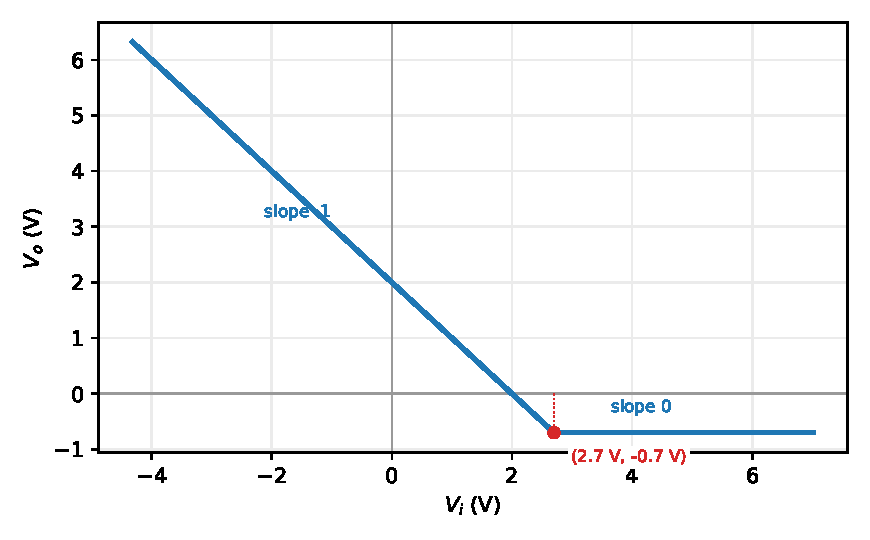
\includegraphics[width=0.62\linewidth,height=6cm,keepaspectratio]{p11_transfer}\end{center}
For $V_i(t) = 4\sin(2\pi\cdot 1000\,t)$ simply pass every instant of $V_i(t)$ through the characteristic above (each piece is a straight line, so each part of the sinusoid is scaled and shifted):\begin{center}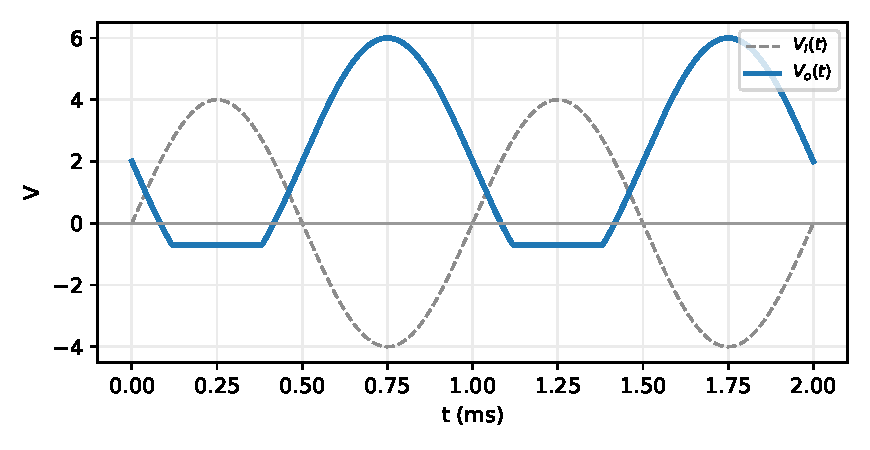
\includegraphics[width=0.62\linewidth,height=5cm,keepaspectratio]{p11_time}\end{center}

\begin{ansbox}
$V_o = \begin{cases} -V_i + 2 & V_i < 2.7 \\ -0.7 & V_i > 2.7 \end{cases}$
\end{ansbox}

\newpage
\subsection*{Solution 3B.12 \hfill Medium}
\begin{center}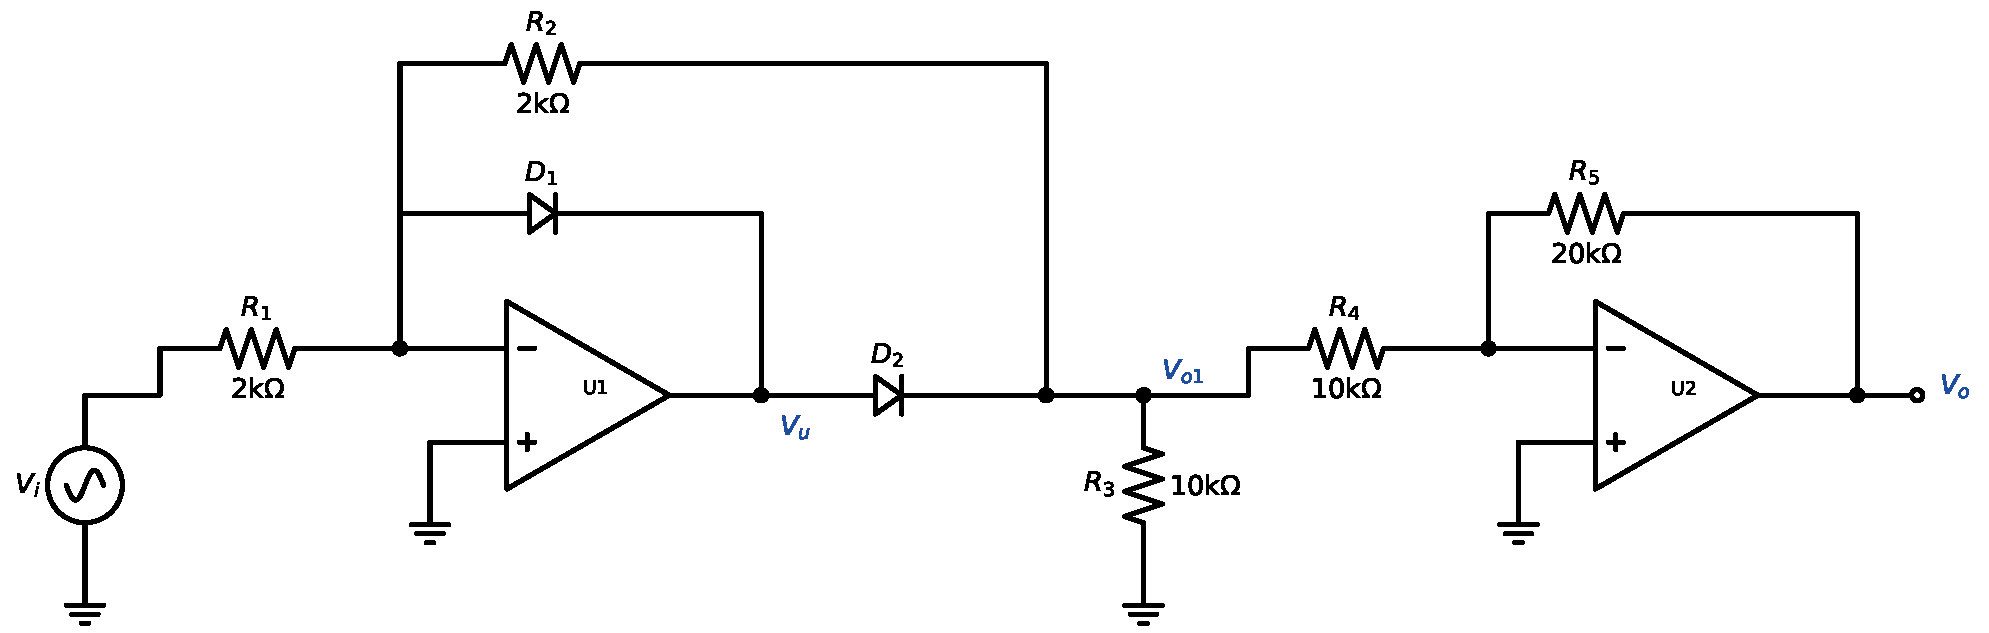
\includegraphics[width=0.9\linewidth,height=5cm,keepaspectratio]{p12_circuit}\end{center}
\solstep{1}{Model and method}Use the constant-voltage-drop model (tool T1): an OFF diode is an open circuit and needs $V_D<0.7$\,V; an ON diode is a $0.7$\,V source and needs $I_D>0$. With 2 diodes there are $4$ ON/OFF combinations. For each one the circuit is linear: solve it with $V_i$ kept as a symbol, then check its assumptions --- each check is a condition on $V_i$ (tool T2). Op-amps are ideal ($A\to\infty$). Whether an op-amp has negative feedback can depend on the diode states, so decide it separately for every combination. Node names used below: $V_{-1}$ = node joining $D_{1}, R_{1}, R_{2}, the op-amp output$; $V_{-2}$ = node joining $R_{4}, R_{5}, the op-amp output$; $V_{o1}$ = node joining $D_{2}, R_{2}, R_{3}, R_{4}$; $V_{u1}$ = node joining $D_{1}, D_{2}, the op-amp output$.
\solstep{2}{Assume $D_{1}$ OFF, $D_{2}$ ON}Replace $D_{1}$ OFF: an open circuit; $D_{2}$ ON: a $0.7$\,V source ($V_{u1} - V_{o1} = 0.7$) carrying an unknown current $I_{D_{2}}$ from anode to cathode. U1 has negative feedback, so $V_- = V_+$ (virtual short) and no current flows into its inputs. U2 has negative feedback, so $V_- = V_+$ (virtual short) and no current flows into its inputs.

Equations (KCL at every node that is not an op-amp output, plus the diode voltages):\begin{align*}
&\text{KCL at }V_{-1}\,(=0): && \frac{0 - V_i}{R_{1}} + \frac{0 - V_{o1}}{R_{2}} = 0 \\
&\text{KCL at }V_{-2}\,(=0): && \frac{0 - V_{o1}}{R_{4}} + \frac{0 - V_{o}}{R_{5}} = 0 \\
&\text{KCL at }V_{o1}: && \frac{V_{o1}}{R_{2}} + \frac{V_{o1}}{R_{3}} + \frac{V_{o1}}{R_{4}} - I_{D_{2}} = 0 \\
&\text{D2 ON}: && V_{u1} - V_{o1} = 0.7
\end{align*}


Solving these linear equations (substitute one into the other, as in Lecture 2) gives, with $V_i$ kept as a symbol:\begin{align*}
V_{o} &= 2V_i \\
V_{D_{1}} = V_{-1} - V_{u1} &= V_i - 0.7 \\
I_{D_{2}} &= -0.7V_i\ \mathrm{mA}
\end{align*}


Check the assumptions: $V_{D_{1}} < 0.7$ $\Rightarrow$ $V_i < 1.4$\,V; $I_{D_{2}} > 0$ $\Rightarrow$ $V_i < 0$\,V. So this state holds for $\boxed{V_i < 0}$, where $V_o = 2V_i$.
\solstep{3}{Assume $D_{1}$ ON, $D_{2}$ OFF}Replace $D_{1}$ ON: a $0.7$\,V source ($V_{-1} - V_{u1} = 0.7$) carrying an unknown current $I_{D_{1}}$ from anode to cathode; $D_{2}$ OFF: an open circuit. U1 has negative feedback, so $V_- = V_+$ (virtual short) and no current flows into its inputs. U2 has negative feedback, so $V_- = V_+$ (virtual short) and no current flows into its inputs.

Equations (KCL at every node that is not an op-amp output, plus the diode voltages):\begin{align*}
&\text{KCL at }V_{-1}\,(=0): && \frac{0 - V_i}{R_{1}} + \frac{0 - V_{o1}}{R_{2}} + I_{D_{1}} = 0 \\
&\text{KCL at }V_{-2}\,(=0): && \frac{0 - V_{o1}}{R_{4}} + \frac{0 - V_{o}}{R_{5}} = 0 \\
&\text{KCL at }V_{o1}: && \frac{V_{o1}}{R_{2}} + \frac{V_{o1}}{R_{3}} + \frac{V_{o1}}{R_{4}} = 0 \\
&\text{D1 ON}: && 0 - V_{u1} = 0.7
\end{align*}


Solving these linear equations (substitute one into the other, as in Lecture 2) gives, with $V_i$ kept as a symbol:\begin{align*}
V_{o} &= 0 \\
I_{D_{1}} &= 0.5V_i\ \mathrm{mA} \\
V_{D_{2}} = V_{u1} - V_{o1} &= -0.7
\end{align*}


Check the assumptions: $I_{D_{1}} > 0$ $\Rightarrow$ $V_i > 0$\,V; $V_{D_{2}} < 0.7$ $\Rightarrow$ true for every $V_i$. So this state holds for $\boxed{V_i > 0}$, where $V_o = 0$.
\solstep{4}{The other combinations}\begin{itemize}[leftmargin=*,itemsep=2pt]
\item $D_{1}$ OFF, $D_{2}$ OFF: $V_{D_{1}}<0.7$ needs $V_i < 0$; $V_{D_{2}}<0.7$ needs $V_i > 0$ --- these cannot all hold, so this state never occurs.
\item $D_{1}$ ON, $D_{2}$ ON: $I_{D_{1}}>0$ needs $V_i > 1.4$; $I_{D_{2}}>0$ is never true --- these cannot all hold, so this state never occurs.
\end{itemize}

\solstep{5}{Assemble and sketch}Put the valid states together:\[
V_o = \begin{cases} 2V_i & V_i < 0 \\ 0 & V_i > 0 \end{cases}
\]
Check: the pieces must meet at each breakpoint --- at $V_i=0$\,V both pieces give $V_o=0$\,V. \checkmark\begin{center}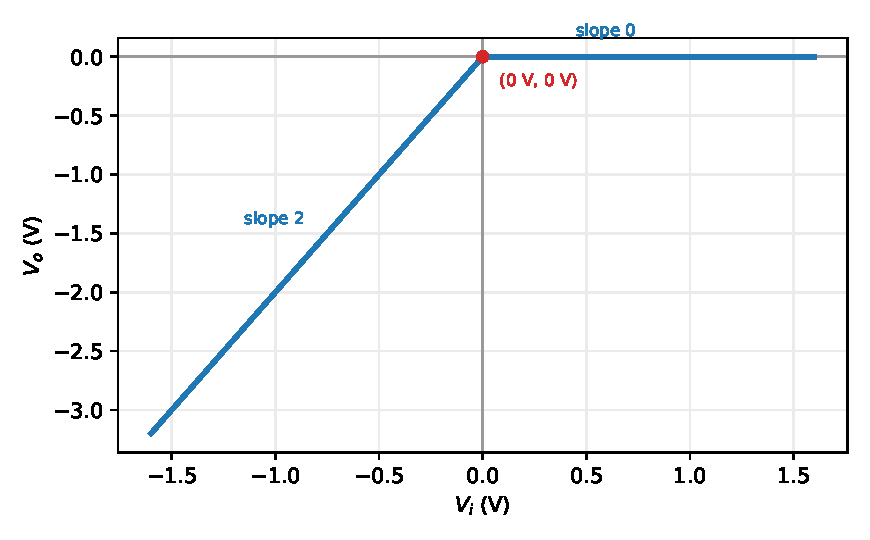
\includegraphics[width=0.62\linewidth,height=6cm,keepaspectratio]{p12_transfer}\end{center}
For $V_i(t) = 1\sin(2\pi\cdot 1000\,t)$ simply pass every instant of $V_i(t)$ through the characteristic above (each piece is a straight line, so each part of the sinusoid is scaled and shifted):\begin{center}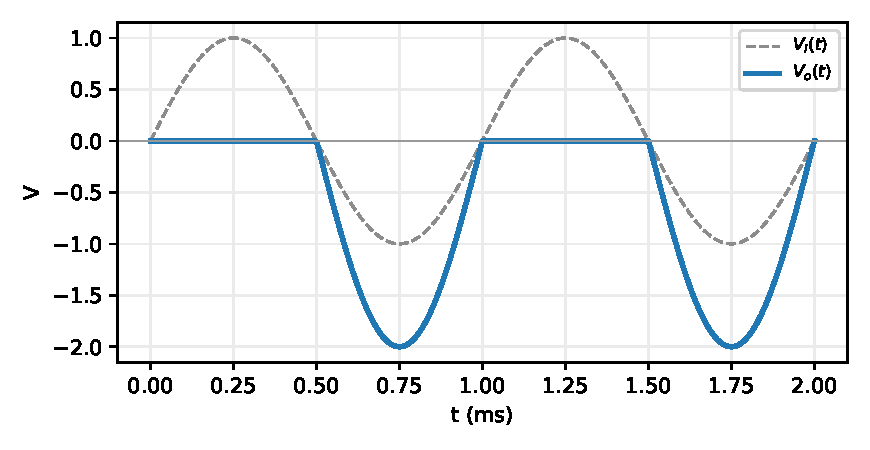
\includegraphics[width=0.62\linewidth,height=5cm,keepaspectratio]{p12_time}\end{center}

\begin{ansbox}
$V_o = \begin{cases} 2V_i & V_i < 0 \\ 0 & V_i > 0 \end{cases}$
\end{ansbox}

\newpage
\subsection*{Solution 3B.13 \hfill Hard}
\begin{center}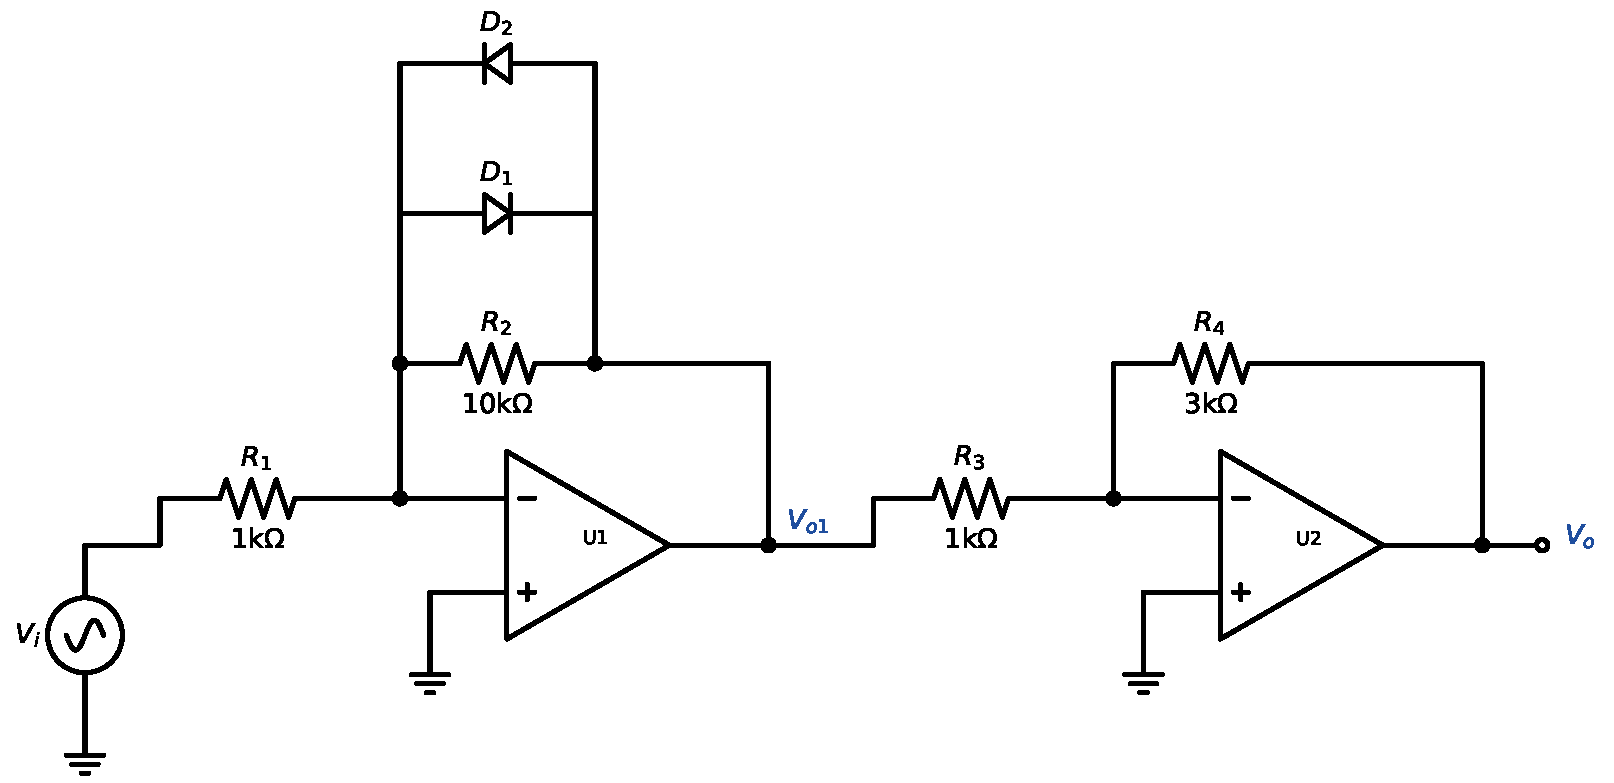
\includegraphics[width=0.9\linewidth,height=5cm,keepaspectratio]{p13_circuit}\end{center}
\solstep{1}{Model and method}Use the constant-voltage-drop model (tool T1): an OFF diode is an open circuit and needs $V_D<0.7$\,V; an ON diode is a $0.7$\,V source and needs $I_D>0$. With 2 diodes there are $4$ ON/OFF combinations. For each one the circuit is linear: solve it with $V_i$ kept as a symbol, then check its assumptions --- each check is a condition on $V_i$ (tool T2). Op-amps are ideal ($A\to\infty$). Whether an op-amp has negative feedback can depend on the diode states, so decide it separately for every combination. Node names used below: $V_{-1}$ = node joining $D_{1}, D_{2}, R_{1}, R_{2}, the op-amp output$; $V_{-2}$ = node joining $R_{3}, R_{4}, the op-amp output$; $V_{o1}$ = node joining $D_{1}, D_{2}, R_{2}, R_{3}, the op-amp output$.
\solstep{2}{Assume $D_{1}$ OFF, $D_{2}$ ON}Replace $D_{1}$ OFF: an open circuit; $D_{2}$ ON: a $0.7$\,V source ($V_{o1} - V_{-1} = 0.7$) carrying an unknown current $I_{D_{2}}$ from anode to cathode. U1 has negative feedback, so $V_- = V_+$ (virtual short) and no current flows into its inputs. U2 has negative feedback, so $V_- = V_+$ (virtual short) and no current flows into its inputs.

Equations (KCL at every node that is not an op-amp output, plus the diode voltages):\begin{align*}
&\text{KCL at }V_{-1}\,(=0): && \frac{0 - V_i}{R_{1}} + \frac{0 - V_{o1}}{R_{2}} - I_{D_{2}} = 0 \\
&\text{KCL at }V_{-2}\,(=0): && \frac{0 - V_{o1}}{R_{3}} + \frac{0 - V_{o}}{R_{4}} = 0 \\
&\text{D2 ON}: && V_{o1} - 0 = 0.7
\end{align*}


Solving these linear equations (substitute one into the other, as in Lecture 2) gives, with $V_i$ kept as a symbol:\begin{align*}
V_{o} &= -2.1 \\
V_{D_{1}} = V_{-1} - V_{o1} &= -0.7 \\
I_{D_{2}} &= -V_i - 0.07\ \mathrm{mA}
\end{align*}


Check the assumptions: $V_{D_{1}} < 0.7$ $\Rightarrow$ true for every $V_i$; $I_{D_{2}} > 0$ $\Rightarrow$ $V_i < -0.07$\,V. So this state holds for $\boxed{V_i < -0.07}$, where $V_o = -2.1$.
\solstep{3}{Assume $D_{1}$ OFF, $D_{2}$ OFF}Replace $D_{1}$ OFF: an open circuit; $D_{2}$ OFF: an open circuit. U1 has negative feedback, so $V_- = V_+$ (virtual short) and no current flows into its inputs. U2 has negative feedback, so $V_- = V_+$ (virtual short) and no current flows into its inputs.

Equations (KCL at every node that is not an op-amp output, plus the diode voltages):\begin{align*}
&\text{KCL at }V_{-1}\,(=0): && \frac{0 - V_i}{R_{1}} + \frac{0 - V_{o1}}{R_{2}} = 0 \\
&\text{KCL at }V_{-2}\,(=0): && \frac{0 - V_{o1}}{R_{3}} + \frac{0 - V_{o}}{R_{4}} = 0
\end{align*}


Solving these linear equations (substitute one into the other, as in Lecture 2) gives, with $V_i$ kept as a symbol:\begin{align*}
V_{o} &= 30V_i \\
V_{D_{1}} = V_{-1} - V_{o1} &= 10V_i \\
V_{D_{2}} = V_{o1} - V_{-1} &= -10V_i
\end{align*}


Check the assumptions: $V_{D_{1}} < 0.7$ $\Rightarrow$ $V_i < 0.07$\,V; $V_{D_{2}} < 0.7$ $\Rightarrow$ $V_i > -0.07$\,V. So this state holds for $\boxed{-0.07 < V_i < 0.07}$, where $V_o = 30V_i$.
\solstep{4}{Assume $D_{1}$ ON, $D_{2}$ OFF}Replace $D_{1}$ ON: a $0.7$\,V source ($V_{-1} - V_{o1} = 0.7$) carrying an unknown current $I_{D_{1}}$ from anode to cathode; $D_{2}$ OFF: an open circuit. U1 has negative feedback, so $V_- = V_+$ (virtual short) and no current flows into its inputs. U2 has negative feedback, so $V_- = V_+$ (virtual short) and no current flows into its inputs.

Equations (KCL at every node that is not an op-amp output, plus the diode voltages):\begin{align*}
&\text{KCL at }V_{-1}\,(=0): && \frac{0 - V_i}{R_{1}} + \frac{0 - V_{o1}}{R_{2}} + I_{D_{1}} = 0 \\
&\text{KCL at }V_{-2}\,(=0): && \frac{0 - V_{o1}}{R_{3}} + \frac{0 - V_{o}}{R_{4}} = 0 \\
&\text{D1 ON}: && 0 - V_{o1} = 0.7
\end{align*}


Solving these linear equations (substitute one into the other, as in Lecture 2) gives, with $V_i$ kept as a symbol:\begin{align*}
V_{o} &= 2.1 \\
I_{D_{1}} &= V_i - 0.07\ \mathrm{mA} \\
V_{D_{2}} = V_{o1} - V_{-1} &= -0.7
\end{align*}


Check the assumptions: $I_{D_{1}} > 0$ $\Rightarrow$ $V_i > 0.07$\,V; $V_{D_{2}} < 0.7$ $\Rightarrow$ true for every $V_i$. So this state holds for $\boxed{V_i > 0.07}$, where $V_o = 2.1$.
\solstep{5}{The other combinations}\begin{itemize}[leftmargin=*,itemsep=2pt]
\item $D_{1}$ ON, $D_{2}$ ON: the ON diodes would have to hold the same node at two different voltages at once, which no circuit can do --- these cannot all hold, so this state never occurs.
\end{itemize}

\solstep{6}{Assemble and sketch}Put the valid states together:\[
V_o = \begin{cases} -2.1 & V_i < -0.07 \\ 30V_i & -0.07 < V_i < 0.07 \\ 2.1 & V_i > 0.07 \end{cases}
\]
Check: the pieces must meet at each breakpoint --- at $V_i=-0.07$\,V both pieces give $V_o=-2.1$\,V; at $V_i=0.07$\,V both pieces give $V_o=2.1$\,V. \checkmark\begin{center}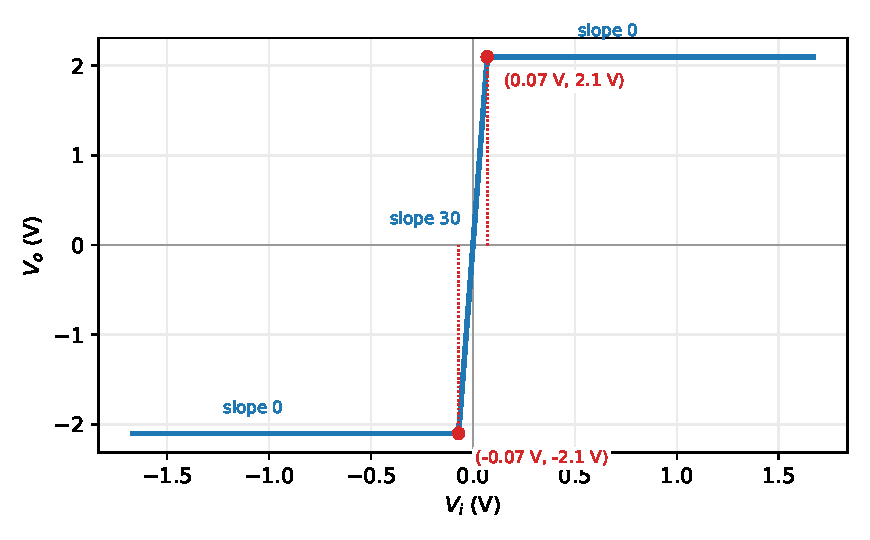
\includegraphics[width=0.62\linewidth,height=6cm,keepaspectratio]{p13_transfer}\end{center}
For $V_i(t) = 0.3\sin(2\pi\cdot 1000\,t)$ simply pass every instant of $V_i(t)$ through the characteristic above (each piece is a straight line, so each part of the sinusoid is scaled and shifted):\begin{center}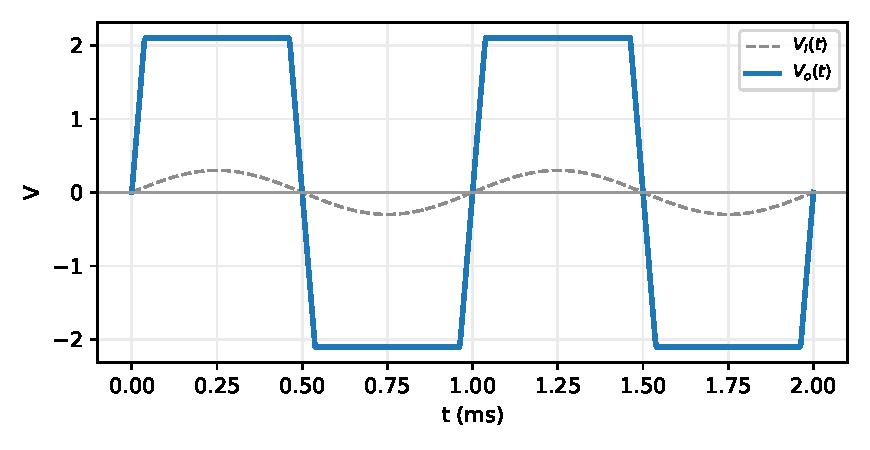
\includegraphics[width=0.62\linewidth,height=5cm,keepaspectratio]{p13_time}\end{center}

\begin{ansbox}
$V_o = \begin{cases} -2.1 & V_i < -0.07 \\ 30V_i & -0.07 < V_i < 0.07 \\ 2.1 & V_i > 0.07 \end{cases}$
\end{ansbox}

\newpage
\subsection*{Solution 3B.14 \hfill Hard}
\begin{center}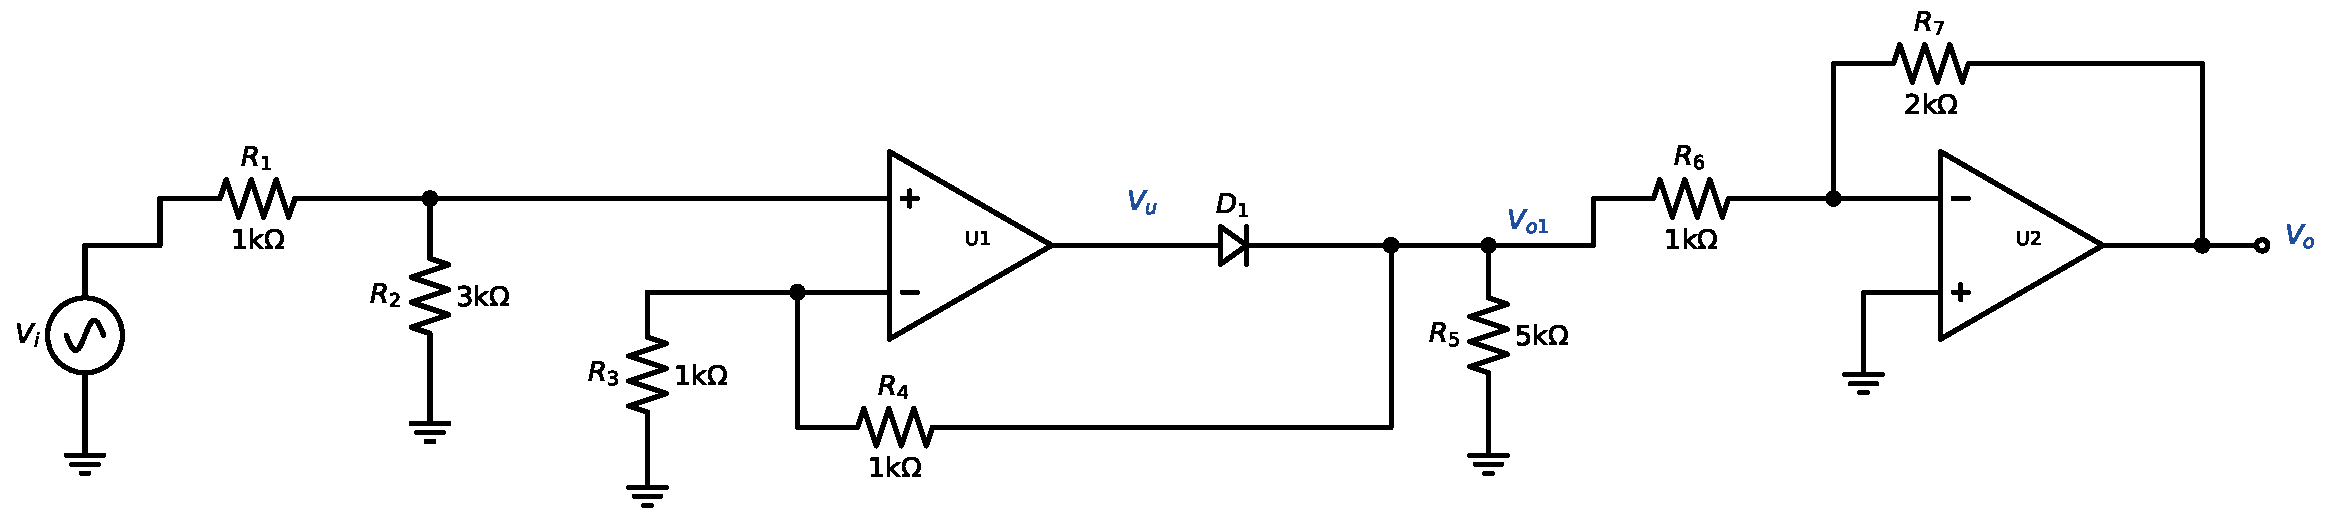
\includegraphics[width=0.9\linewidth,height=5cm,keepaspectratio]{p14_circuit}\end{center}
\solstep{1}{Model and method}Use the constant-voltage-drop model (tool T1): an OFF diode is an open circuit and needs $V_D<0.7$\,V; an ON diode is a $0.7$\,V source and needs $I_D>0$. With 1 diode there are $2$ ON/OFF combinations. For each one the circuit is linear: solve it with $V_i$ kept as a symbol, then check its assumptions --- each check is a condition on $V_i$ (tool T2). Op-amps are ideal ($A\to\infty$). Whether an op-amp has negative feedback can depend on the diode states, so decide it separately for every combination. Node names used below: $V_{+1}$ = node joining $R_{1}, R_{2}, the op-amp output$; $V_{-1}$ = node joining $R_{3}, R_{4}, the op-amp output$; $V_{-2}$ = node joining $R_{6}, R_{7}, the op-amp output$; $V_{o1}$ = node joining $D_{1}, R_{4}, R_{5}, R_{6}$; $V_{u1}$ = node joining $D_{1}, the op-amp output$.
\solstep{2}{Assume $D_{1}$ OFF}Replace $D_{1}$ OFF: an open circuit. With this assumption U1 has no feedback path from its output back to its $-$ input: it runs \emph{open-loop}, $V_{u1} = A(V_+ - V_-)$ with $A\to\infty$, so its output is pushed to $\pm\infty$ (in practice, a supply rail) unless $V_+ = V_-$ exactly. U2 has negative feedback, so $V_- = V_+$ (virtual short) and no current flows into its inputs.

Equations (KCL at every node that is not an op-amp output, plus the diode voltages):\begin{align*}
&\text{KCL at }V_{+1}: && \frac{V_{+1} - V_i}{R_{1}} + \frac{V_{+1}}{R_{2}} = 0 \\
&\text{KCL at }V_{-1}: && \frac{V_{-1}}{R_{3}} + \frac{V_{-1} - V_{o1}}{R_{4}} = 0 \\
&\text{KCL at }V_{-2}\,(=0): && \frac{0 - V_{o1}}{R_{6}} + \frac{0 - V_{o}}{R_{7}} = 0 \\
&\text{KCL at }V_{o1}: && \frac{V_{o1} - V_{-1}}{R_{4}} + \frac{V_{o1}}{R_{5}} + \frac{V_{o1}}{R_{6}} = 0
\end{align*}


Solving these linear equations (substitute one into the other, as in Lecture 2) gives, with $V_i$ kept as a symbol:\begin{align*}
V_{o} &= 0 \\
V_{D_{1}} = V_{u1} - V_{o1} &\approx A\left(0.75V_i\right)
\end{align*}


Check the assumptions: $V_{D_{1}} < 0.7$; since $A\to\infty$ this needs $0.75V_i < 0$ $\Rightarrow$ $V_i < 0$\,V. So this state holds for $\boxed{V_i < 0}$, where $V_o = 0$.
\solstep{3}{Assume $D_{1}$ ON}Replace $D_{1}$ ON: a $0.7$\,V source ($V_{u1} - V_{o1} = 0.7$) carrying an unknown current $I_{D_{1}}$ from anode to cathode. U1 has negative feedback, so $V_- = V_+$ (virtual short) and no current flows into its inputs. U2 has negative feedback, so $V_- = V_+$ (virtual short) and no current flows into its inputs.

Equations (KCL at every node that is not an op-amp output, plus the diode voltages):\begin{align*}
&\text{KCL at }V_{+1}: && \frac{V_{+1} - V_i}{R_{1}} + \frac{V_{+1}}{R_{2}} = 0 \\
&\text{KCL at }V_{-1}\,(=V_{+1}): && \frac{V_{+1}}{R_{3}} + \frac{V_{+1} - V_{o1}}{R_{4}} = 0 \\
&\text{KCL at }V_{-2}\,(=0): && \frac{0 - V_{o1}}{R_{6}} + \frac{0 - V_{o}}{R_{7}} = 0 \\
&\text{KCL at }V_{o1}: && \frac{V_{o1} - V_{+1}}{R_{4}} + \frac{V_{o1}}{R_{5}} + \frac{V_{o1}}{R_{6}} - I_{D_{1}} = 0 \\
&\text{D1 ON}: && V_{u1} - V_{o1} = 0.7
\end{align*}


Solving these linear equations (substitute one into the other, as in Lecture 2) gives, with $V_i$ kept as a symbol:\begin{align*}
V_{o} &= -3V_i \\
I_{D_{1}} &= 2.55V_i\ \mathrm{mA}
\end{align*}


Check the assumptions: $I_{D_{1}} > 0$ $\Rightarrow$ $V_i > 0$\,V. So this state holds for $\boxed{V_i > 0}$, where $V_o = -3V_i$.
\solstep{4}{Assemble and sketch}Put the valid states together:\[
V_o = \begin{cases} 0 & V_i < 0 \\ -3V_i & V_i > 0 \end{cases}
\]
Check: the pieces must meet at each breakpoint --- at $V_i=0$\,V both pieces give $V_o=0$\,V. \checkmark\begin{center}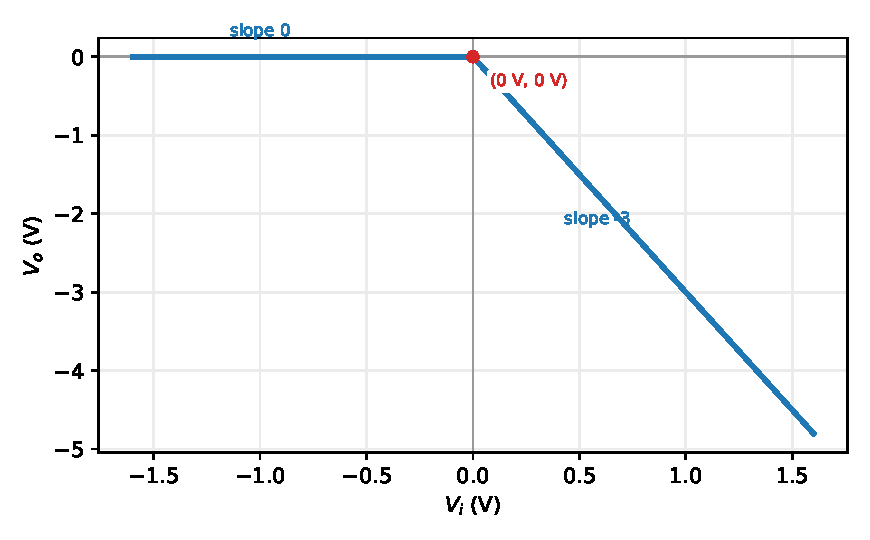
\includegraphics[width=0.62\linewidth,height=6cm,keepaspectratio]{p14_transfer}\end{center}
For $V_i(t) = 1\sin(2\pi\cdot 500\,t)$ simply pass every instant of $V_i(t)$ through the characteristic above (each piece is a straight line, so each part of the sinusoid is scaled and shifted):\begin{center}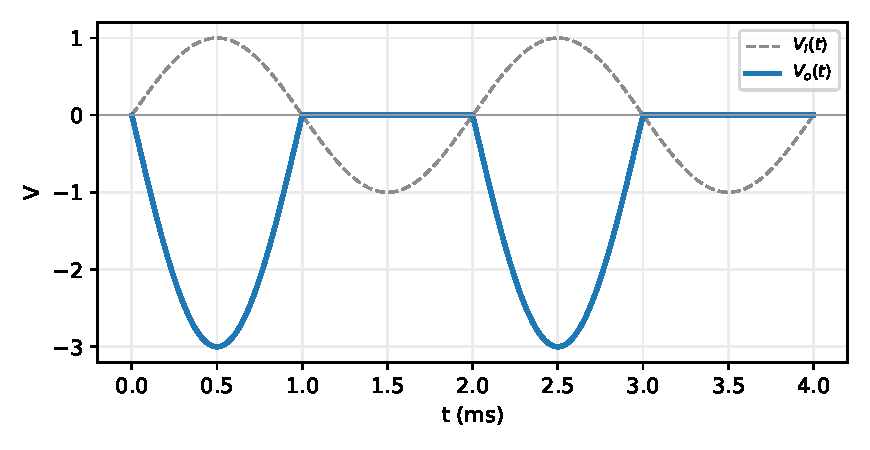
\includegraphics[width=0.62\linewidth,height=5cm,keepaspectratio]{p14_time}\end{center}

\begin{ansbox}
$V_o = \begin{cases} 0 & V_i < 0 \\ -3V_i & V_i > 0 \end{cases}$
\end{ansbox}

\newpage
\subsection*{Solution 3B.15 \hfill Hard}
\begin{center}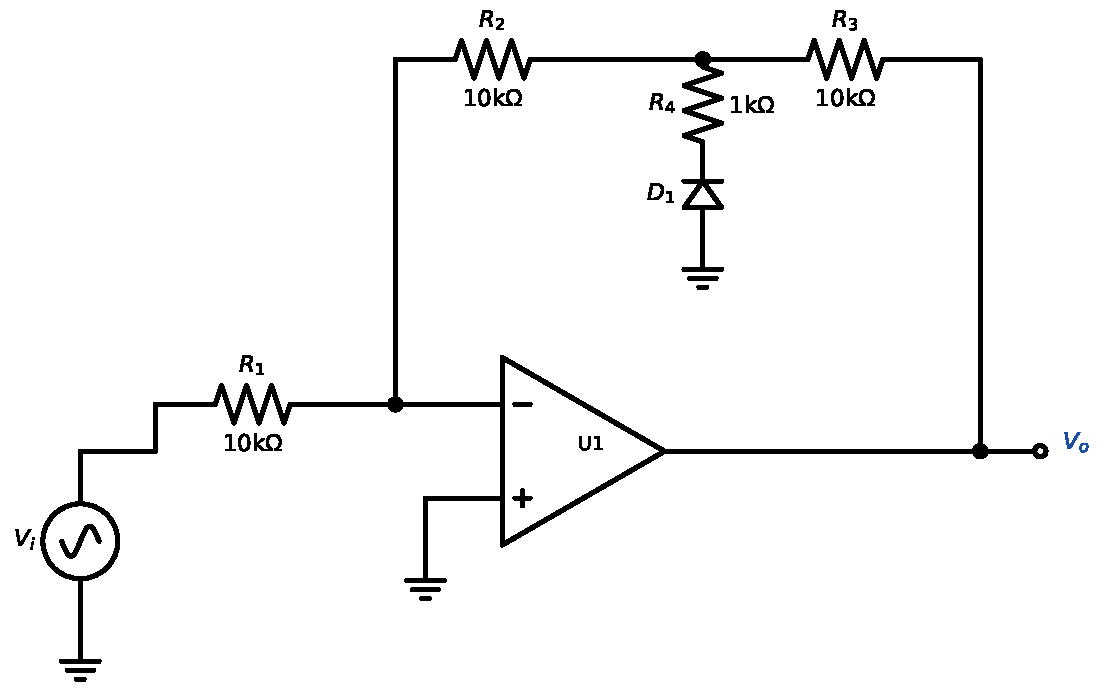
\includegraphics[width=0.9\linewidth,height=5cm,keepaspectratio]{p15_circuit}\end{center}
\solstep{1}{Model and method}Use the constant-voltage-drop model (tool T1): an OFF diode is an open circuit and needs $V_D<0.7$\,V; an ON diode is a $0.7$\,V source and needs $I_D>0$. With 1 diode there are $2$ ON/OFF combinations. For each one the circuit is linear: solve it with $V_i$ kept as a symbol, then check its assumptions --- each check is a condition on $V_i$ (tool T2). Op-amps are ideal ($A\to\infty$). Whether an op-amp has negative feedback can depend on the diode states, so decide it separately for every combination. Node names used below: $V_{-}$ = the op-amp's $-$ input; $V_{a}$ = node joining $D_{1}, R_{4}$; $V_{b}$ = node joining $R_{2}, R_{3}, R_{4}$.
\solstep{2}{Assume $D_{1}$ OFF}Replace $D_{1}$ OFF: an open circuit. U1 has negative feedback, so $V_- = V_+$ (virtual short) and no current flows into its inputs.

Equations (KCL at every node that is not an op-amp output, plus the diode voltages):\begin{align*}
&\text{KCL at }V_{-}\,(=0): && \frac{0 - V_i}{R_{1}} + \frac{0 - V_{b}}{R_{2}} = 0 \\
&\text{KCL at }V_{a}: && \frac{V_{a} - V_{b}}{R_{4}} = 0 \\
&\text{KCL at }V_{b}: && \frac{V_{b}}{R_{2}} + \frac{V_{b} - V_{o}}{R_{3}} + \frac{V_{b} - V_{a}}{R_{4}} = 0
\end{align*}


Solving these linear equations (substitute one into the other, as in Lecture 2) gives, with $V_i$ kept as a symbol:\begin{align*}
V_{o} &= -2V_i \\
V_{D_{1}} = 0 - V_{a} &= V_i
\end{align*}


Check the assumptions: $V_{D_{1}} < 0.7$ $\Rightarrow$ $V_i < 0.7$\,V. So this state holds for $\boxed{V_i < 0.7}$, where $V_o = -2V_i$.
\solstep{3}{Assume $D_{1}$ ON}Replace $D_{1}$ ON: a $0.7$\,V source ($0 - V_{a} = 0.7$) carrying an unknown current $I_{D_{1}}$ from anode to cathode. U1 has negative feedback, so $V_- = V_+$ (virtual short) and no current flows into its inputs.

Equations (KCL at every node that is not an op-amp output, plus the diode voltages):\begin{align*}
&\text{KCL at }V_{-}\,(=0): && \frac{0 - V_i}{R_{1}} + \frac{0 - V_{b}}{R_{2}} = 0 \\
&\text{KCL at }V_{a}: && \frac{V_{a} - V_{b}}{R_{4}} - I_{D_{1}} = 0 \\
&\text{KCL at }V_{b}: && \frac{V_{b}}{R_{2}} + \frac{V_{b} - V_{o}}{R_{3}} + \frac{V_{b} - V_{a}}{R_{4}} = 0 \\
&\text{D1 ON}: && 0 - V_{a} = 0.7
\end{align*}


Solving these linear equations (substitute one into the other, as in Lecture 2) gives, with $V_i$ kept as a symbol:\begin{align*}
V_{o} &= -12V_i + 7 \\
I_{D_{1}} &= V_i - 0.7\ \mathrm{mA}
\end{align*}


Check the assumptions: $I_{D_{1}} > 0$ $\Rightarrow$ $V_i > 0.7$\,V. So this state holds for $\boxed{V_i > 0.7}$, where $V_o = -12V_i + 7$.
\solstep{4}{Assemble and sketch}Put the valid states together:\[
V_o = \begin{cases} -2V_i & V_i < 0.7 \\ -12V_i + 7 & V_i > 0.7 \end{cases}
\]
Check: the pieces must meet at each breakpoint --- at $V_i=0.7$\,V both pieces give $V_o=-1.4$\,V. \checkmark\begin{center}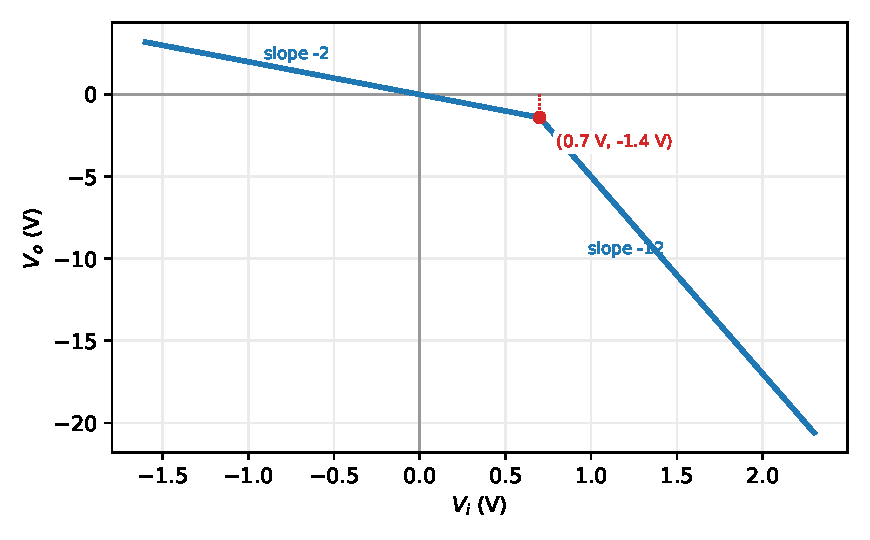
\includegraphics[width=0.62\linewidth,height=6cm,keepaspectratio]{p15_transfer}\end{center}
For $V_i(t) = 1\sin(2\pi\cdot 1000\,t)$ simply pass every instant of $V_i(t)$ through the characteristic above (each piece is a straight line, so each part of the sinusoid is scaled and shifted):\begin{center}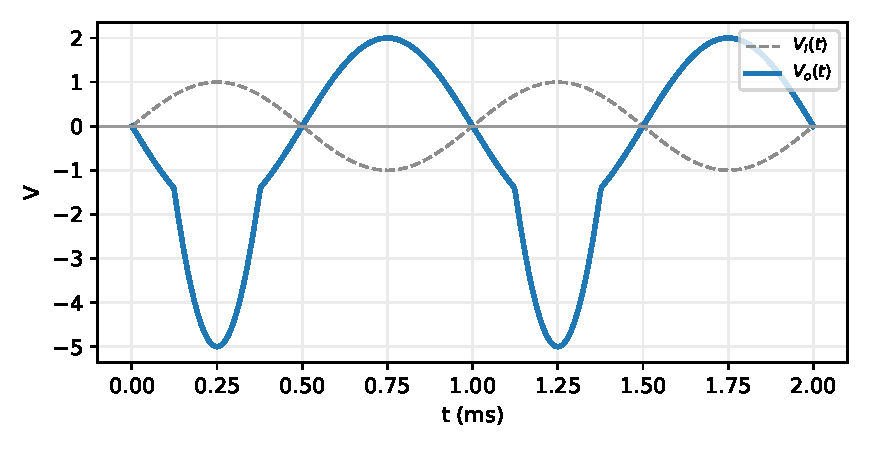
\includegraphics[width=0.62\linewidth,height=5cm,keepaspectratio]{p15_time}\end{center}

\begin{ansbox}
$V_o = \begin{cases} -2V_i & V_i < 0.7 \\ -12V_i + 7 & V_i > 0.7 \end{cases}$
\end{ansbox}

\newpage
\subsection*{Solution 3B.16 \hfill Hard}
\begin{center}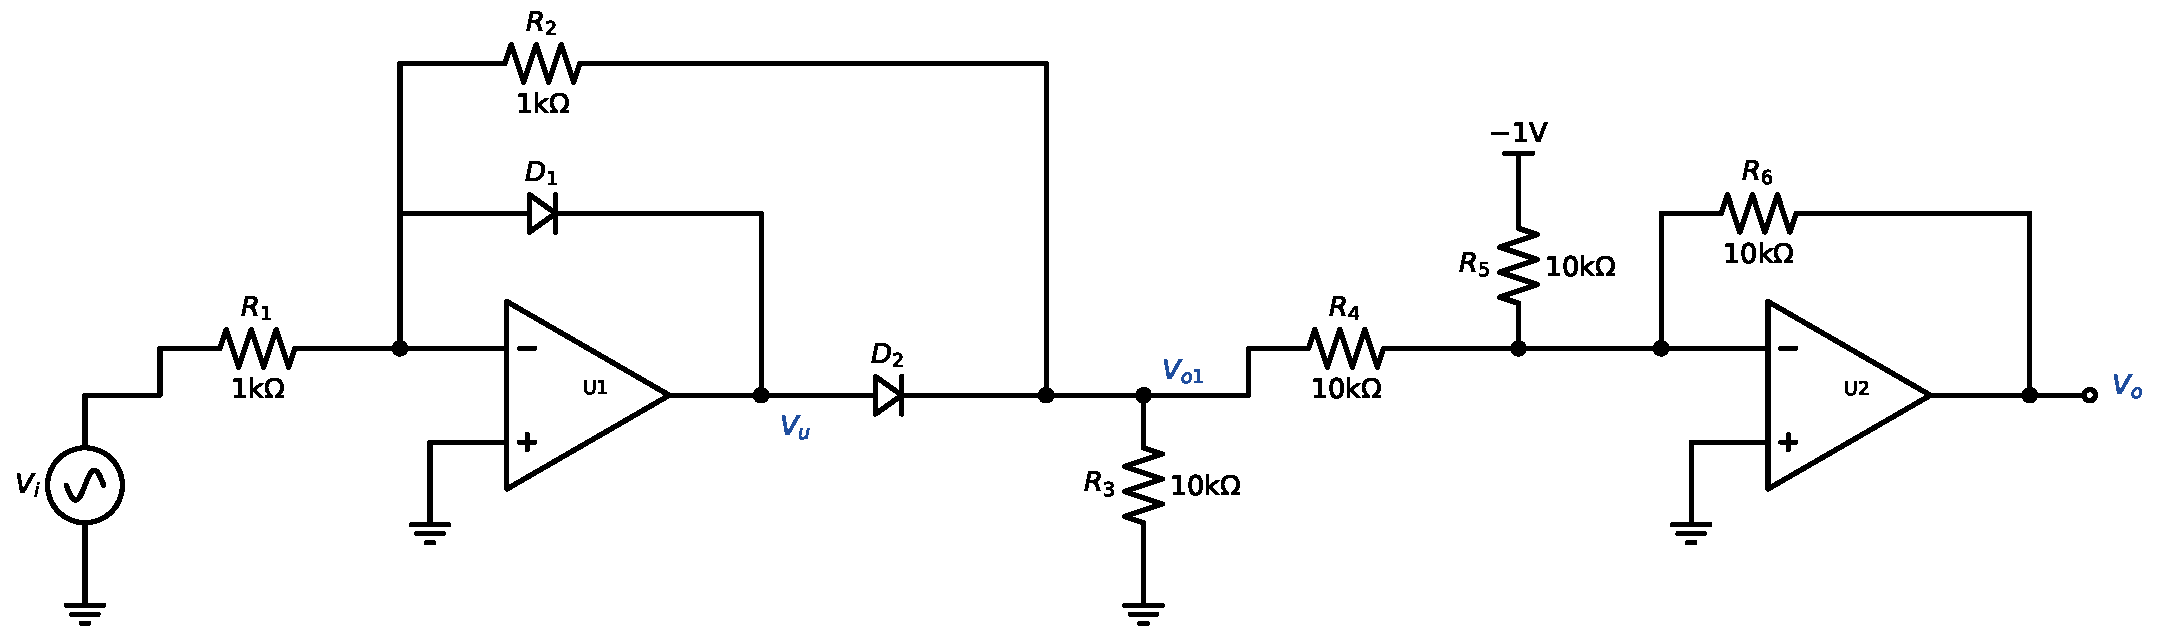
\includegraphics[width=0.9\linewidth,height=5cm,keepaspectratio]{p16_circuit}\end{center}
\solstep{1}{Model and method}Use the constant-voltage-drop model (tool T1): an OFF diode is an open circuit and needs $V_D<0.7$\,V; an ON diode is a $0.7$\,V source and needs $I_D>0$. With 2 diodes there are $4$ ON/OFF combinations. For each one the circuit is linear: solve it with $V_i$ kept as a symbol, then check its assumptions --- each check is a condition on $V_i$ (tool T2). Op-amps are ideal ($A\to\infty$). Whether an op-amp has negative feedback can depend on the diode states, so decide it separately for every combination. Node names used below: $V_{-1}$ = node joining $D_{1}, R_{1}, R_{2}, the op-amp output$; $V_{-2}$ = node joining $R_{4}, R_{5}, R_{6}, the op-amp output$; $V_{o1}$ = node joining $D_{2}, R_{2}, R_{3}, R_{4}$; $V_{u1}$ = node joining $D_{1}, D_{2}, the op-amp output$.
\solstep{2}{Assume $D_{1}$ OFF, $D_{2}$ ON}Replace $D_{1}$ OFF: an open circuit; $D_{2}$ ON: a $0.7$\,V source ($V_{u1} - V_{o1} = 0.7$) carrying an unknown current $I_{D_{2}}$ from anode to cathode. U1 has negative feedback, so $V_- = V_+$ (virtual short) and no current flows into its inputs. U2 has negative feedback, so $V_- = V_+$ (virtual short) and no current flows into its inputs.

Equations (KCL at every node that is not an op-amp output, plus the diode voltages):\begin{align*}
&\text{KCL at }V_{-1}\,(=0): && \frac{0 - V_i}{R_{1}} + \frac{0 - V_{o1}}{R_{2}} = 0 \\
&\text{KCL at }V_{-2}\,(=0): && \frac{0 - V_{o1}}{R_{4}} + \frac{0 - V_{o}}{R_{6}} + \frac{0 - -1}{R_{5}} = 0 \\
&\text{KCL at }V_{o1}: && \frac{V_{o1}}{R_{2}} + \frac{V_{o1}}{R_{3}} + \frac{V_{o1}}{R_{4}} - I_{D_{2}} = 0 \\
&\text{D2 ON}: && V_{u1} - V_{o1} = 0.7
\end{align*}


Solving these linear equations (substitute one into the other, as in Lecture 2) gives, with $V_i$ kept as a symbol:\begin{align*}
V_{o} &= V_i + 1 \\
V_{D_{1}} = V_{-1} - V_{u1} &= V_i - 0.7 \\
I_{D_{2}} &= -1.2V_i\ \mathrm{mA}
\end{align*}


Check the assumptions: $V_{D_{1}} < 0.7$ $\Rightarrow$ $V_i < 1.4$\,V; $I_{D_{2}} > 0$ $\Rightarrow$ $V_i < 0$\,V. So this state holds for $\boxed{V_i < 0}$, where $V_o = V_i + 1$.
\solstep{3}{Assume $D_{1}$ ON, $D_{2}$ OFF}Replace $D_{1}$ ON: a $0.7$\,V source ($V_{-1} - V_{u1} = 0.7$) carrying an unknown current $I_{D_{1}}$ from anode to cathode; $D_{2}$ OFF: an open circuit. U1 has negative feedback, so $V_- = V_+$ (virtual short) and no current flows into its inputs. U2 has negative feedback, so $V_- = V_+$ (virtual short) and no current flows into its inputs.

Equations (KCL at every node that is not an op-amp output, plus the diode voltages):\begin{align*}
&\text{KCL at }V_{-1}\,(=0): && \frac{0 - V_i}{R_{1}} + \frac{0 - V_{o1}}{R_{2}} + I_{D_{1}} = 0 \\
&\text{KCL at }V_{-2}\,(=0): && \frac{0 - V_{o1}}{R_{4}} + \frac{0 - V_{o}}{R_{6}} + \frac{0 - -1}{R_{5}} = 0 \\
&\text{KCL at }V_{o1}: && \frac{V_{o1}}{R_{2}} + \frac{V_{o1}}{R_{3}} + \frac{V_{o1}}{R_{4}} = 0 \\
&\text{D1 ON}: && 0 - V_{u1} = 0.7
\end{align*}


Solving these linear equations (substitute one into the other, as in Lecture 2) gives, with $V_i$ kept as a symbol:\begin{align*}
V_{o} &= 1 \\
I_{D_{1}} &= V_i\ \mathrm{mA} \\
V_{D_{2}} = V_{u1} - V_{o1} &= -0.7
\end{align*}


Check the assumptions: $I_{D_{1}} > 0$ $\Rightarrow$ $V_i > 0$\,V; $V_{D_{2}} < 0.7$ $\Rightarrow$ true for every $V_i$. So this state holds for $\boxed{V_i > 0}$, where $V_o = 1$.
\solstep{4}{The other combinations}\begin{itemize}[leftmargin=*,itemsep=2pt]
\item $D_{1}$ OFF, $D_{2}$ OFF: $V_{D_{1}}<0.7$ needs $V_i < 0$; $V_{D_{2}}<0.7$ needs $V_i > 0$ --- these cannot all hold, so this state never occurs.
\item $D_{1}$ ON, $D_{2}$ ON: $I_{D_{1}}>0$ needs $V_i > 1.4$; $I_{D_{2}}>0$ is never true --- these cannot all hold, so this state never occurs.
\end{itemize}

\solstep{5}{Assemble and sketch}Put the valid states together:\[
V_o = \begin{cases} V_i + 1 & V_i < 0 \\ 1 & V_i > 0 \end{cases}
\]
Check: the pieces must meet at each breakpoint --- at $V_i=0$\,V both pieces give $V_o=1$\,V. \checkmark\begin{center}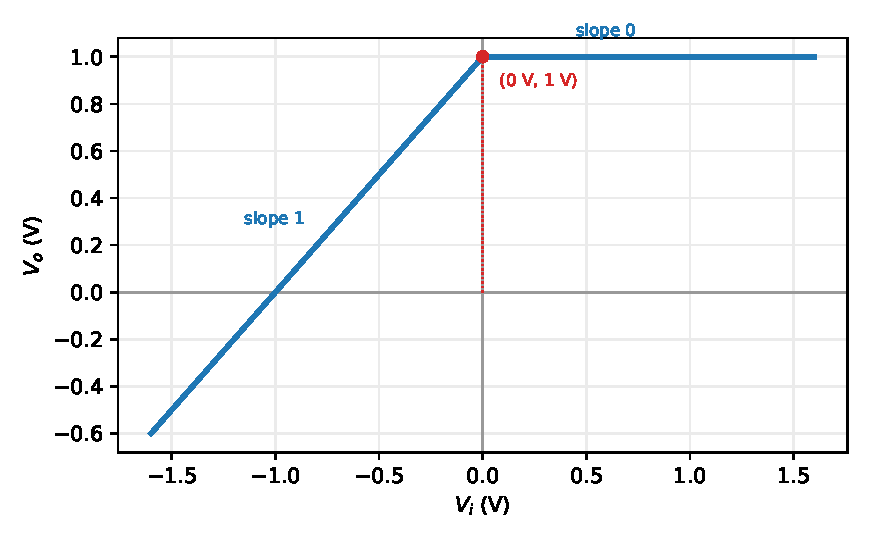
\includegraphics[width=0.62\linewidth,height=6cm,keepaspectratio]{p16_transfer}\end{center}
For $V_i(t) = 2\sin(2\pi\cdot 1000\,t)$ simply pass every instant of $V_i(t)$ through the characteristic above (each piece is a straight line, so each part of the sinusoid is scaled and shifted):\begin{center}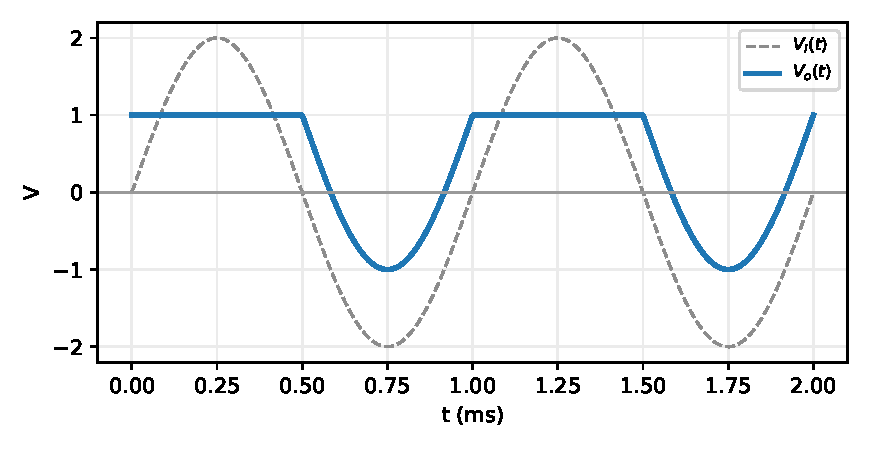
\includegraphics[width=0.62\linewidth,height=5cm,keepaspectratio]{p16_time}\end{center}

\begin{ansbox}
$V_o = \begin{cases} V_i + 1 & V_i < 0 \\ 1 & V_i > 0 \end{cases}$
\end{ansbox}

\newpage
\subsection*{Solution 3B.17 \hfill Hard}
\begin{center}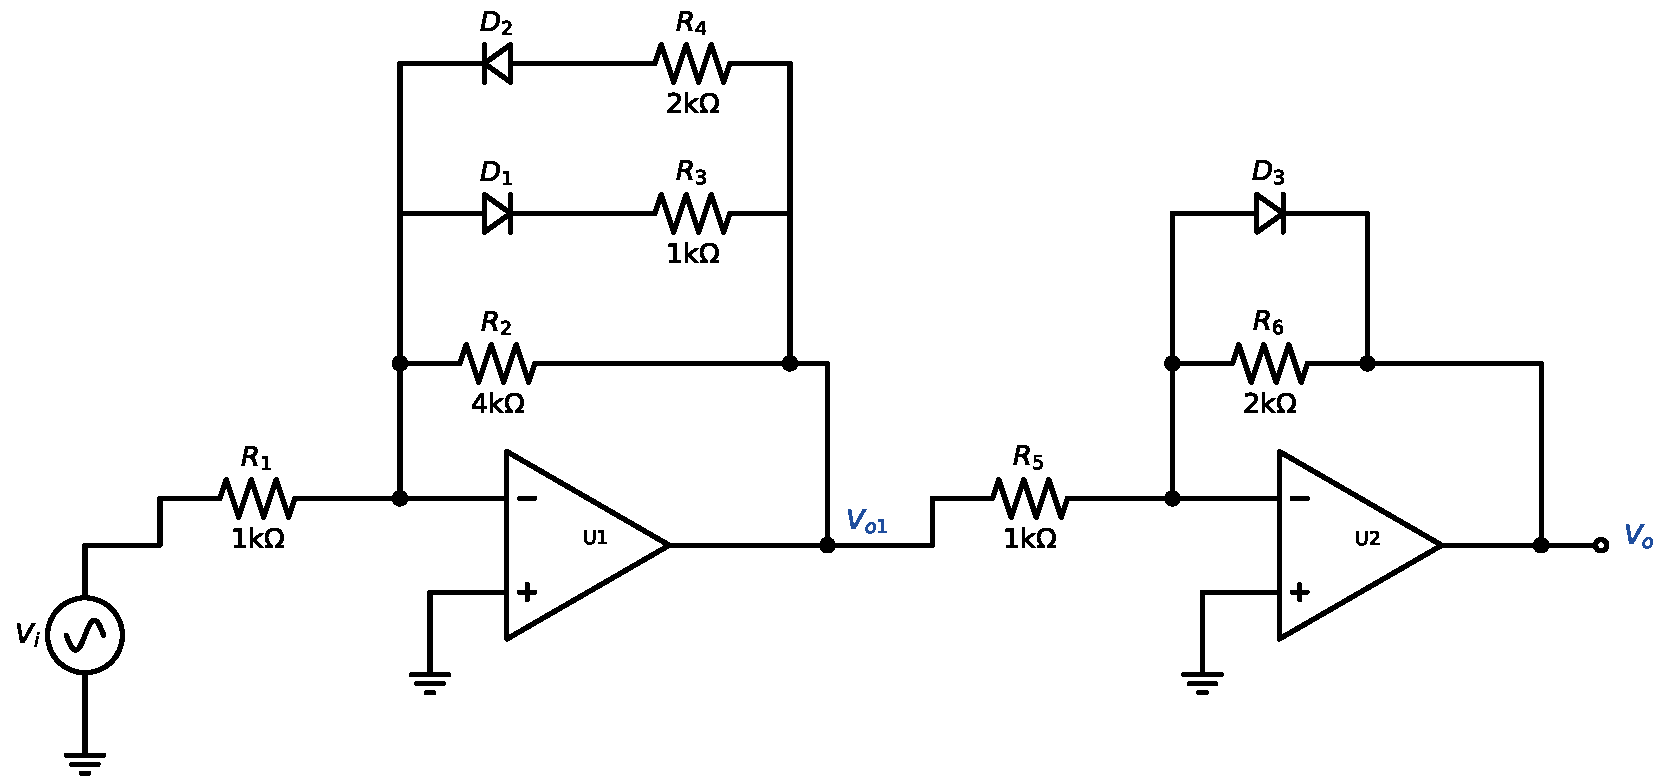
\includegraphics[width=0.9\linewidth,height=5cm,keepaspectratio]{p17_circuit}\end{center}
\solstep{1}{Model and method}Use the constant-voltage-drop model (tool T1): an OFF diode is an open circuit and needs $V_D<0.7$\,V; an ON diode is a $0.7$\,V source and needs $I_D>0$. With 3 diodes there are $8$ ON/OFF combinations. For each one the circuit is linear: solve it with $V_i$ kept as a symbol, then check its assumptions --- each check is a condition on $V_i$ (tool T2). Op-amps are ideal ($A\to\infty$). Whether an op-amp has negative feedback can depend on the diode states, so decide it separately for every combination. Node names used below: $V_{-1}$ = node joining $D_{1}, D_{2}, R_{1}, R_{2}, the op-amp output$; $V_{-2}$ = node joining $D_{3}, R_{5}, R_{6}, the op-amp output$; $V_{a}$ = node joining $D_{1}, R_{3}$; $V_{b}$ = node joining $D_{2}, R_{4}$; $V_{o1}$ = node joining $R_{2}, R_{3}, R_{4}, R_{5}, the op-amp output$.
\solstep{2}{Assume $D_{1}$ OFF, $D_{2}$ ON, $D_{3}$ ON}Replace $D_{1}$ OFF: an open circuit; $D_{2}$ ON: a $0.7$\,V source ($V_{b} - V_{-1} = 0.7$) carrying an unknown current $I_{D_{2}}$ from anode to cathode; $D_{3}$ ON: a $0.7$\,V source ($V_{-2} - V_{o} = 0.7$) carrying an unknown current $I_{D_{3}}$ from anode to cathode. U1 has negative feedback, so $V_- = V_+$ (virtual short) and no current flows into its inputs. U2 has negative feedback, so $V_- = V_+$ (virtual short) and no current flows into its inputs.

Equations (KCL at every node that is not an op-amp output, plus the diode voltages):\begin{align*}
&\text{KCL at }V_{-1}\,(=0): && \frac{0 - V_i}{R_{1}} + \frac{0 - V_{o1}}{R_{2}} - I_{D_{2}} = 0 \\
&\text{KCL at }V_{-2}\,(=0): && \frac{0 - V_{o1}}{R_{5}} + \frac{0 - V_{o}}{R_{6}} + I_{D_{3}} = 0 \\
&\text{KCL at }V_{a}: && \frac{V_{a} - V_{o1}}{R_{3}} = 0 \\
&\text{KCL at }V_{b}: && \frac{V_{b} - V_{o1}}{R_{4}} + I_{D_{2}} = 0 \\
&\text{D2 ON}: && V_{b} - 0 = 0.7 \\
&\text{D3 ON}: && 0 - V_{o} = 0.7
\end{align*}


Solving these linear equations (substitute one into the other, as in Lecture 2) gives, with $V_i$ kept as a symbol:\begin{align*}
V_{o} &= -0.7 \\
V_{D_{1}} = V_{-1} - V_{a} &= 1.333V_i - 0.4667 \\
I_{D_{2}} &= -0.6667V_i - 0.1167\ \mathrm{mA} \\
I_{D_{3}} &= -1.333V_i + 0.1167\ \mathrm{mA}
\end{align*}


Check the assumptions: $V_{D_{1}} < 0.7$ $\Rightarrow$ $V_i < 0.875$\,V; $I_{D_{2}} > 0$ $\Rightarrow$ $V_i < -0.175$\,V; $I_{D_{3}} > 0$ $\Rightarrow$ $V_i < 0.0875$\,V. So this state holds for $\boxed{V_i < -0.175}$, where $V_o = -0.7$.
\solstep{3}{Assume $D_{1}$ OFF, $D_{2}$ OFF, $D_{3}$ ON}Replace $D_{1}$ OFF: an open circuit; $D_{2}$ OFF: an open circuit; $D_{3}$ ON: a $0.7$\,V source ($V_{-2} - V_{o} = 0.7$) carrying an unknown current $I_{D_{3}}$ from anode to cathode. U1 has negative feedback, so $V_- = V_+$ (virtual short) and no current flows into its inputs. U2 has negative feedback, so $V_- = V_+$ (virtual short) and no current flows into its inputs.

Equations (KCL at every node that is not an op-amp output, plus the diode voltages):\begin{align*}
&\text{KCL at }V_{-1}\,(=0): && \frac{0 - V_i}{R_{1}} + \frac{0 - V_{o1}}{R_{2}} = 0 \\
&\text{KCL at }V_{-2}\,(=0): && \frac{0 - V_{o1}}{R_{5}} + \frac{0 - V_{o}}{R_{6}} + I_{D_{3}} = 0 \\
&\text{KCL at }V_{a}: && \frac{V_{a} - V_{o1}}{R_{3}} = 0 \\
&\text{KCL at }V_{b}: && \frac{V_{b} - V_{o1}}{R_{4}} = 0 \\
&\text{D3 ON}: && 0 - V_{o} = 0.7
\end{align*}


Solving these linear equations (substitute one into the other, as in Lecture 2) gives, with $V_i$ kept as a symbol:\begin{align*}
V_{o} &= -0.7 \\
V_{D_{1}} = V_{-1} - V_{a} &= 4V_i \\
V_{D_{2}} = V_{b} - V_{-1} &= -4V_i \\
I_{D_{3}} &= -4V_i - 0.35\ \mathrm{mA}
\end{align*}


Check the assumptions: $V_{D_{1}} < 0.7$ $\Rightarrow$ $V_i < 0.175$\,V; $V_{D_{2}} < 0.7$ $\Rightarrow$ $V_i > -0.175$\,V; $I_{D_{3}} > 0$ $\Rightarrow$ $V_i < -0.0875$\,V. So this state holds for $\boxed{-0.175 < V_i < -0.0875}$, where $V_o = -0.7$.
\solstep{4}{Assume $D_{1}$ OFF, $D_{2}$ OFF, $D_{3}$ OFF}Replace $D_{1}$ OFF: an open circuit; $D_{2}$ OFF: an open circuit; $D_{3}$ OFF: an open circuit. U1 has negative feedback, so $V_- = V_+$ (virtual short) and no current flows into its inputs. U2 has negative feedback, so $V_- = V_+$ (virtual short) and no current flows into its inputs.

Equations (KCL at every node that is not an op-amp output, plus the diode voltages):\begin{align*}
&\text{KCL at }V_{-1}\,(=0): && \frac{0 - V_i}{R_{1}} + \frac{0 - V_{o1}}{R_{2}} = 0 \\
&\text{KCL at }V_{-2}\,(=0): && \frac{0 - V_{o1}}{R_{5}} + \frac{0 - V_{o}}{R_{6}} = 0 \\
&\text{KCL at }V_{a}: && \frac{V_{a} - V_{o1}}{R_{3}} = 0 \\
&\text{KCL at }V_{b}: && \frac{V_{b} - V_{o1}}{R_{4}} = 0
\end{align*}


Solving these linear equations (substitute one into the other, as in Lecture 2) gives, with $V_i$ kept as a symbol:\begin{align*}
V_{o} &= 8V_i \\
V_{D_{1}} = V_{-1} - V_{a} &= 4V_i \\
V_{D_{2}} = V_{b} - V_{-1} &= -4V_i \\
V_{D_{3}} = V_{-2} - V_{o} &= -8V_i
\end{align*}


Check the assumptions: $V_{D_{1}} < 0.7$ $\Rightarrow$ $V_i < 0.175$\,V; $V_{D_{2}} < 0.7$ $\Rightarrow$ $V_i > -0.175$\,V; $V_{D_{3}} < 0.7$ $\Rightarrow$ $V_i > -0.0875$\,V. So this state holds for $\boxed{-0.0875 < V_i < 0.175}$, where $V_o = 8V_i$.
\solstep{5}{Assume $D_{1}$ ON, $D_{2}$ OFF, $D_{3}$ OFF}Replace $D_{1}$ ON: a $0.7$\,V source ($V_{-1} - V_{a} = 0.7$) carrying an unknown current $I_{D_{1}}$ from anode to cathode; $D_{2}$ OFF: an open circuit; $D_{3}$ OFF: an open circuit. U1 has negative feedback, so $V_- = V_+$ (virtual short) and no current flows into its inputs. U2 has negative feedback, so $V_- = V_+$ (virtual short) and no current flows into its inputs.

Equations (KCL at every node that is not an op-amp output, plus the diode voltages):\begin{align*}
&\text{KCL at }V_{-1}\,(=0): && \frac{0 - V_i}{R_{1}} + \frac{0 - V_{o1}}{R_{2}} + I_{D_{1}} = 0 \\
&\text{KCL at }V_{-2}\,(=0): && \frac{0 - V_{o1}}{R_{5}} + \frac{0 - V_{o}}{R_{6}} = 0 \\
&\text{KCL at }V_{a}: && \frac{V_{a} - V_{o1}}{R_{3}} - I_{D_{1}} = 0 \\
&\text{KCL at }V_{b}: && \frac{V_{b} - V_{o1}}{R_{4}} = 0 \\
&\text{D1 ON}: && 0 - V_{a} = 0.7
\end{align*}


Solving these linear equations (substitute one into the other, as in Lecture 2) gives, with $V_i$ kept as a symbol:\begin{align*}
V_{o} &= 1.6V_i + 1.12 \\
I_{D_{1}} &= 0.8V_i - 0.14\ \mathrm{mA} \\
V_{D_{2}} = V_{b} - V_{-1} &= -0.8V_i - 0.56 \\
V_{D_{3}} = V_{-2} - V_{o} &= -1.6V_i - 1.12
\end{align*}


Check the assumptions: $I_{D_{1}} > 0$ $\Rightarrow$ $V_i > 0.175$\,V; $V_{D_{2}} < 0.7$ $\Rightarrow$ $V_i > -1.575$\,V; $V_{D_{3}} < 0.7$ $\Rightarrow$ $V_i > -1.137$\,V. So this state holds for $\boxed{V_i > 0.175}$, where $V_o = 1.6V_i + 1.12$.
\solstep{6}{The other combinations}\begin{itemize}[leftmargin=*,itemsep=2pt]
\item $D_{1}$ OFF, $D_{2}$ ON, $D_{3}$ OFF: $V_{D_{1}}<0.7$ needs $V_i < 0.875$; $I_{D_{2}}>0$ needs $V_i < -0.175$; $V_{D_{3}}<0.7$ needs $V_i > 0.0875$ --- these cannot all hold, so this state never occurs.
\item $D_{1}$ ON, $D_{2}$ OFF, $D_{3}$ ON: $I_{D_{1}}>0$ needs $V_i > 0.175$; $V_{D_{2}}<0.7$ needs $V_i > -1.575$; $I_{D_{3}}>0$ needs $V_i < -1.137$ --- these cannot all hold, so this state never occurs.
\item $D_{1}$ ON, $D_{2}$ ON, $D_{3}$ OFF: $I_{D_{1}}>0$ needs $V_i > 0.875$; $I_{D_{2}}>0$ needs $V_i < -1.575$; $V_{D_{3}}<0.7$ needs $V_i > -0.9625$ --- these cannot all hold, so this state never occurs.
\item $D_{1}$ ON, $D_{2}$ ON, $D_{3}$ ON: $I_{D_{1}}>0$ needs $V_i > 0.875$; $I_{D_{2}}>0$ needs $V_i < -1.575$; $I_{D_{3}}>0$ needs $V_i < -0.9625$ --- these cannot all hold, so this state never occurs.
\end{itemize}

\solstep{7}{Assemble and sketch}Put the valid states together (neighbouring states that give the \emph{same} $V_o$ are merged: a diode changes state there, but it does not affect $V_o$):\[
V_o = \begin{cases} -0.7 & V_i < -0.0875 \\ 8V_i & -0.0875 < V_i < 0.175 \\ 1.6V_i + 1.12 & V_i > 0.175 \end{cases}
\]
Check: the pieces must meet at each breakpoint --- at $V_i=-0.0875$\,V both pieces give $V_o=-0.7$\,V; at $V_i=0.175$\,V both pieces give $V_o=1.4$\,V. \checkmark\begin{center}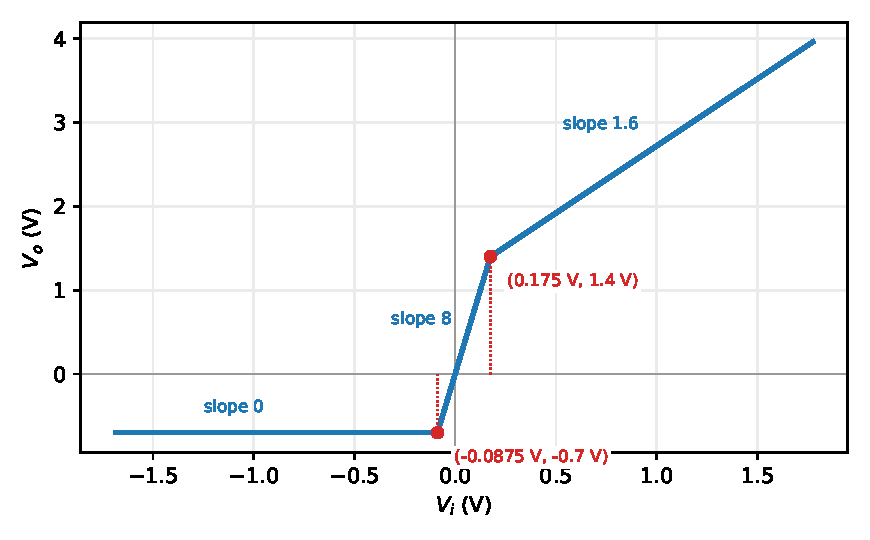
\includegraphics[width=0.62\linewidth,height=6cm,keepaspectratio]{p17_transfer}\end{center}
For $V_i(t) = 2\sin(2\pi\cdot 1000\,t)$ simply pass every instant of $V_i(t)$ through the characteristic above (each piece is a straight line, so each part of the sinusoid is scaled and shifted):\begin{center}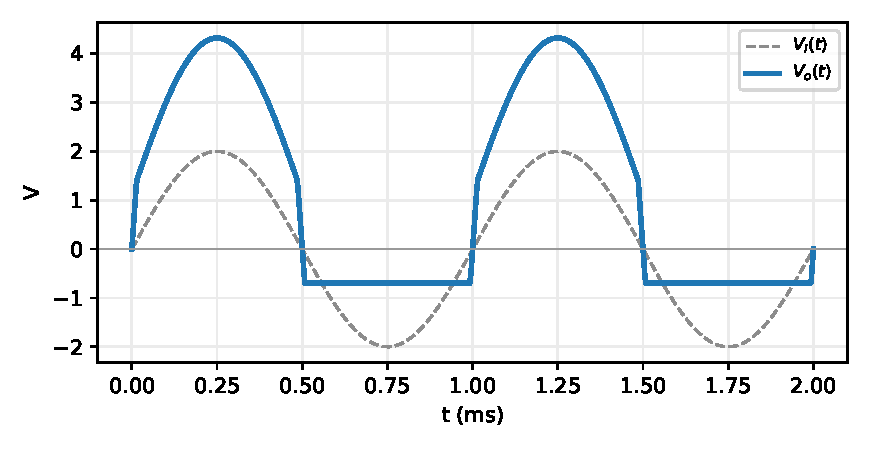
\includegraphics[width=0.62\linewidth,height=5cm,keepaspectratio]{p17_time}\end{center}

\begin{ansbox}
$V_o = \begin{cases} -0.7 & V_i < -0.0875 \\ 8V_i & -0.0875 < V_i < 0.175 \\ 1.6V_i + 1.12 & V_i > 0.175 \end{cases}$
\end{ansbox}

\newpage
\subsection*{Solution 3B.18 \hfill Hard}
\begin{center}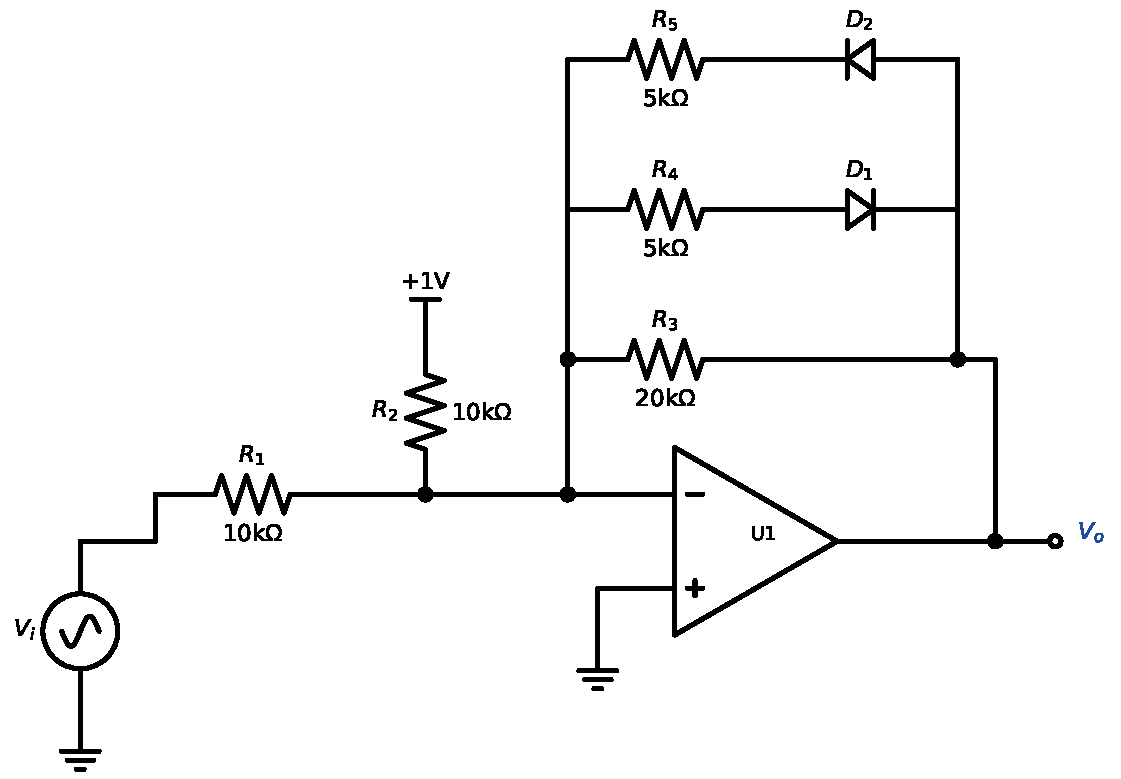
\includegraphics[width=0.9\linewidth,height=5cm,keepaspectratio]{p18_circuit}\end{center}
\solstep{1}{Model and method}Use the constant-voltage-drop model (tool T1): an OFF diode is an open circuit and needs $V_D<0.7$\,V; an ON diode is a $0.7$\,V source and needs $I_D>0$. With 2 diodes there are $4$ ON/OFF combinations. For each one the circuit is linear: solve it with $V_i$ kept as a symbol, then check its assumptions --- each check is a condition on $V_i$ (tool T2). Op-amps are ideal ($A\to\infty$). Whether an op-amp has negative feedback can depend on the diode states, so decide it separately for every combination. Node names used below: $V_{-}$ = the op-amp's $-$ input; $V_{a}$ = node joining $D_{1}, R_{4}$; $V_{b}$ = node joining $D_{2}, R_{5}$.
\solstep{2}{Assume $D_{1}$ OFF, $D_{2}$ ON}Replace $D_{1}$ OFF: an open circuit; $D_{2}$ ON: a $0.7$\,V source ($V_{o} - V_{b} = 0.7$) carrying an unknown current $I_{D_{2}}$ from anode to cathode. U1 has negative feedback, so $V_- = V_+$ (virtual short) and no current flows into its inputs.

Equations (KCL at every node that is not an op-amp output, plus the diode voltages):\begin{align*}
&\text{KCL at }V_{-}\,(=0): && \frac{0 - V_i}{R_{1}} + \frac{0 - V_{o}}{R_{3}} + \frac{0 - V_{a}}{R_{4}} + \frac{0 - V_{b}}{R_{5}} + \frac{0 - 1}{R_{2}} = 0 \\
&\text{KCL at }V_{a}: && \frac{V_{a}}{R_{4}} = 0 \\
&\text{KCL at }V_{b}: && \frac{V_{b}}{R_{5}} - I_{D_{2}} = 0 \\
&\text{D2 ON}: && V_{o} - V_{b} = 0.7
\end{align*}


Solving these linear equations (substitute one into the other, as in Lecture 2) gives, with $V_i$ kept as a symbol:\begin{align*}
V_{o} &= -0.4V_i + 0.16 \\
V_{D_{1}} = V_{a} - V_{o} &= 0.4V_i - 0.16 \\
I_{D_{2}} &= -0.08V_i - 0.108\ \mathrm{mA}
\end{align*}


Check the assumptions: $V_{D_{1}} < 0.7$ $\Rightarrow$ $V_i < 2.15$\,V; $I_{D_{2}} > 0$ $\Rightarrow$ $V_i < -1.35$\,V. So this state holds for $\boxed{V_i < -1.35}$, where $V_o = -0.4V_i + 0.16$.
\solstep{3}{Assume $D_{1}$ OFF, $D_{2}$ OFF}Replace $D_{1}$ OFF: an open circuit; $D_{2}$ OFF: an open circuit. U1 has negative feedback, so $V_- = V_+$ (virtual short) and no current flows into its inputs.

Equations (KCL at every node that is not an op-amp output, plus the diode voltages):\begin{align*}
&\text{KCL at }V_{-}\,(=0): && \frac{0 - V_i}{R_{1}} + \frac{0 - V_{o}}{R_{3}} + \frac{0 - V_{a}}{R_{4}} + \frac{0 - V_{b}}{R_{5}} + \frac{0 - 1}{R_{2}} = 0 \\
&\text{KCL at }V_{a}: && \frac{V_{a}}{R_{4}} = 0 \\
&\text{KCL at }V_{b}: && \frac{V_{b}}{R_{5}} = 0
\end{align*}


Solving these linear equations (substitute one into the other, as in Lecture 2) gives, with $V_i$ kept as a symbol:\begin{align*}
V_{o} &= -2V_i - 2 \\
V_{D_{1}} = V_{a} - V_{o} &= 2V_i + 2 \\
V_{D_{2}} = V_{o} - V_{b} &= -2V_i - 2
\end{align*}


Check the assumptions: $V_{D_{1}} < 0.7$ $\Rightarrow$ $V_i < -0.65$\,V; $V_{D_{2}} < 0.7$ $\Rightarrow$ $V_i > -1.35$\,V. So this state holds for $\boxed{-1.35 < V_i < -0.65}$, where $V_o = -2V_i - 2$.
\solstep{4}{Assume $D_{1}$ ON, $D_{2}$ OFF}Replace $D_{1}$ ON: a $0.7$\,V source ($V_{a} - V_{o} = 0.7$) carrying an unknown current $I_{D_{1}}$ from anode to cathode; $D_{2}$ OFF: an open circuit. U1 has negative feedback, so $V_- = V_+$ (virtual short) and no current flows into its inputs.

Equations (KCL at every node that is not an op-amp output, plus the diode voltages):\begin{align*}
&\text{KCL at }V_{-}\,(=0): && \frac{0 - V_i}{R_{1}} + \frac{0 - V_{o}}{R_{3}} + \frac{0 - V_{a}}{R_{4}} + \frac{0 - V_{b}}{R_{5}} + \frac{0 - 1}{R_{2}} = 0 \\
&\text{KCL at }V_{a}: && \frac{V_{a}}{R_{4}} + I_{D_{1}} = 0 \\
&\text{KCL at }V_{b}: && \frac{V_{b}}{R_{5}} = 0 \\
&\text{D1 ON}: && V_{a} - V_{o} = 0.7
\end{align*}


Solving these linear equations (substitute one into the other, as in Lecture 2) gives, with $V_i$ kept as a symbol:\begin{align*}
V_{o} &= -0.4V_i - 0.96 \\
I_{D_{1}} &= 0.08V_i + 0.052\ \mathrm{mA} \\
V_{D_{2}} = V_{o} - V_{b} &= -0.4V_i - 0.96
\end{align*}


Check the assumptions: $I_{D_{1}} > 0$ $\Rightarrow$ $V_i > -0.65$\,V; $V_{D_{2}} < 0.7$ $\Rightarrow$ $V_i > -4.15$\,V. So this state holds for $\boxed{V_i > -0.65}$, where $V_o = -0.4V_i - 0.96$.
\solstep{5}{The other combinations}\begin{itemize}[leftmargin=*,itemsep=2pt]
\item $D_{1}$ ON, $D_{2}$ ON: $I_{D_{1}}>0$ needs $V_i > 2.15$; $I_{D_{2}}>0$ needs $V_i < -4.15$ --- these cannot all hold, so this state never occurs.
\end{itemize}

\solstep{6}{Assemble and sketch}Put the valid states together:\[
V_o = \begin{cases} -0.4V_i + 0.16 & V_i < -1.35 \\ -2V_i - 2 & -1.35 < V_i < -0.65 \\ -0.4V_i - 0.96 & V_i > -0.65 \end{cases}
\]
Check: the pieces must meet at each breakpoint --- at $V_i=-1.35$\,V both pieces give $V_o=0.7$\,V; at $V_i=-0.65$\,V both pieces give $V_o=-0.7$\,V. \checkmark\begin{center}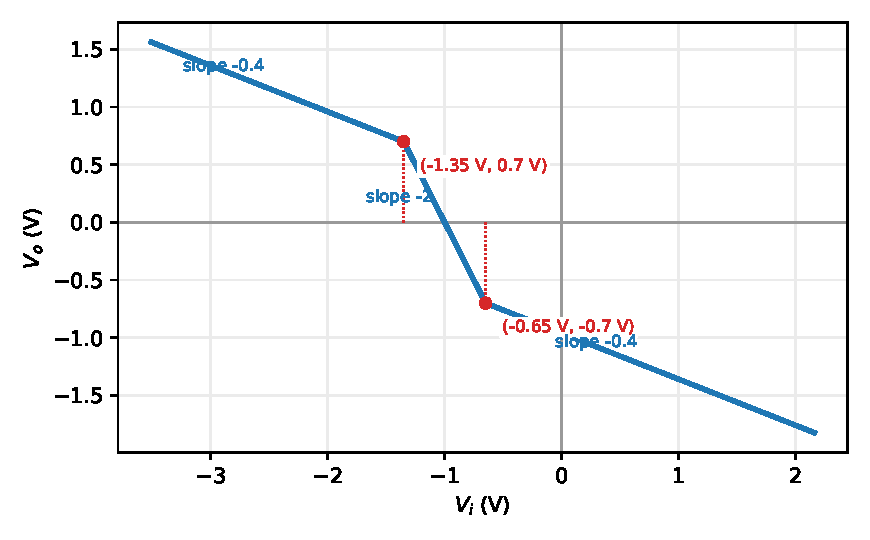
\includegraphics[width=0.62\linewidth,height=6cm,keepaspectratio]{p18_transfer}\end{center}
For $V_i(t) = 3\sin(2\pi\cdot 1000\,t)$ simply pass every instant of $V_i(t)$ through the characteristic above (each piece is a straight line, so each part of the sinusoid is scaled and shifted):\begin{center}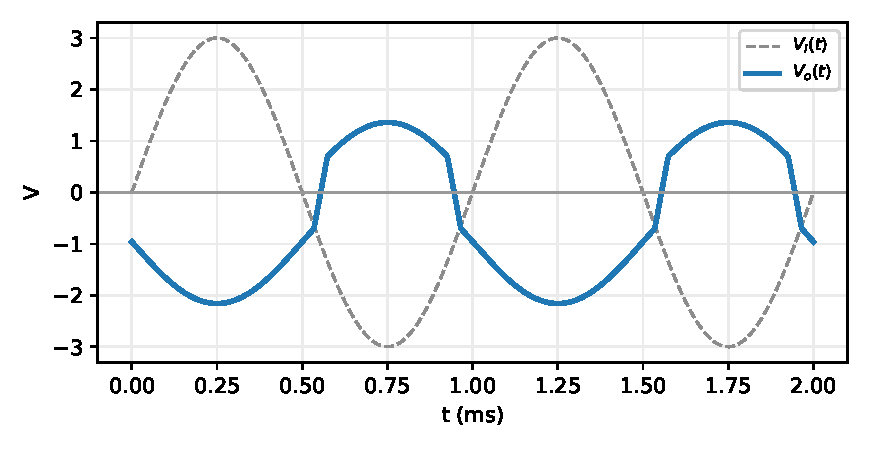
\includegraphics[width=0.62\linewidth,height=5cm,keepaspectratio]{p18_time}\end{center}

\begin{ansbox}
$V_o = \begin{cases} -0.4V_i + 0.16 & V_i < -1.35 \\ -2V_i - 2 & -1.35 < V_i < -0.65 \\ -0.4V_i - 0.96 & V_i > -0.65 \end{cases}$
\end{ansbox}

\end{document}
